\chapter{\gtest\ descriptions}
\label{chap:gtestdescription}
%For understanding grid electron emission in the \lze\ detector, we designed a gaseous xenon detector to study grid behavior in a similar environment as in the \lze\ detector. We measure electron emission rate from the grid under different grid operating voltages. It helps us figure out the optimal operating voltages for grids in the \lze\ detector. We study different method for reducing electron emission background. Reduction of electron emission background rate from the grid wires will  improve our sensitivity to low energy events. This in return will improve our understanding of low mass WIMPs. It will also help to keep the trigger environment in \lze\ quieter. This reduces the systematic errors for S1 and S2 and improve their quality. From that, we will improve our events classification and energy reconstruction. 

%Understanding electron emission processes from the grids in the \lze\ detector, and reducing the rate of this process are essential for the operation of the \lze\ detector. Among all different electron emission processes, 

In LZ, metallic wire grids under high voltage are used to form electric fields. We apply one field in the liquid volume to drift ionization electrons upwards and another in the gas volume to extract these electrons from the liquid in order to produce proportional scintillation light (S2). Achieving high voltages on such grids is necessary for the operation of the LZ TPC. However, such high voltages also increase the rate of electron emission ,which is one of the potential sources of background in LZ.
%\lze\ is particularly interested in electric field induced electron emission from the metallic grid. This phenomenon is one of the major sources of background events. 
Therefore, reduction of the field induced electron emission rate should greatly benefit physics studies in the \lze\ detector.

Electric field induced electron emission from metallic surfaces is a well known phenomenon. The electric field lowers the potential energy outside the metallic surface allowing electrons to come out from the metallic surface. The rate of electric field induced electron emission increases with the electric field on the metallic surface. 


%has been difficult in the past for other liquid xenon TPCs. The difficulty limiting the high voltage breakdown on the grids and other metallic surfaces, but also in limiting electron emission from these surfaces.  


The electric field induced electron emission events are potential problems in LZ for three reasons. First, these events look like low energy events in the \lze\ detector. Thus, reduction of electron emission background rate from the grid wires improves our sensitivity to low energy events. This in turn improves our ability to study low mass WIMPs. 
Second, the electron emission events may accidentally coincide with WIMP signals which we want to study in the \lze\ detector. Reduction of electron emission rate helps to keep the data recording environment in \lze\ cleaner. This reduces the systematic errors for S1 and S2 and improves their quality. From that, we improve our events classification and energy reconstruction. This in turn improves all physics studies using the \lze\ detector. 
Finally, the electron emission events interrupt the desired data recording capability of the \lze\ detector. This may prevent or interrupt recordings of wanted data. Thus, the reduction of electron emission rate helps to keep the data recording environment in \lze\ quieter to allow longer detector live times for wanted events.
In summary, the reduction of the electron emission event rates benefits LZ because of its impact on detector sensitivity, data quality and data acquisition live time. 
%The maximum operating electric field on the grids in the \lze\ elector set the maximum grids operation voltages. 

To achieve these qualities, we are developing a two-stage study on the reduction of the electric field induced electron emission rate using two small detectors, \gtest\ and \phaseone . These two detectors are capable of testing a pair of grids which have surface areas  \SI{\sim 1}{\percent} the area of grids that will be used in \lze . With these small detectors, we can study the effect of rate reduction in a shorter time than if we were to use full-size grids. Thus, we use these detectors to study parameters that may affect the emission rate in a short period of time.

At the first stage, a gaseous detector, ``\gtest ", is built to study different methods for reducing the electron emission rate. This detector measures electron emission rates with different electric fields before and after various physical and chemical treatments. Once we discover an effect on the reduction of the electric field induced electron emission rate from these treatments, a second stage of study with a liquid xenon detector, \phaseone , is undertaken to confirm that reduction persists in a liquid xenon environment, like that of \lze. 

After confirmation that a treatment produces a rate reduction,  this treatment is used to produce full-size \lze\ grids. A similar two-stage study method is used to test the full-size LZ grids in a gaseous detector, \phasetwo(details are described in Ref.~\ref{whose thesis}), and the liquid xenon detector \lze . These two detectors measure the performance and assure the quality of LZ grids.

%This chapter focus on \gtest .
%This detector measures scintillation and electroluminescence (EL) light signals from events in the detector. This detector operates with gaseous xenon, gaseous argon, and vacuum.  
%We measure electron emission rate from the grid under different grid operating voltages. It helps us figure out the optimal operating voltages for grids in the \lze\ detector. We study different method for reducing electron emission background.
%consist with two major parts: the operating system and data acquisition system. 

%The operating system contains four parts: the tested grids, the gas handling and distribution system, the high voltage system and the light collection system. The gas handling and distribution system is for delivering and storing quality pure gas to the \gtest\ . It includes the operating chamber, the gas circulation panel and plumbing, pressure and temperature sensors of different range, and a separated purity measurement system. The high voltage system includes the power supply, high voltage feed-through, cables, and cable termination. The light collection system for measuring the quantity of scintillation light created in the detector includes two PMTs, and the PTFE light reflector.

%The data acquisition(DAQ) system is attached directly onto the output of the two PMTs. It does PMT pulse amplification, shaping, digitizing, transferring and storing.   

%The recorded events were passed to a data processing framework to reduce the dimensions of the input data. Then, the reduced quantity data(RQs) were sent for event classification to select the interesting events. Because of the rate of the electron emission event we are mostly interested in has a various range, in some case really rare. A studying of background events for its the pulse shape, and energy distribution were done to reduce the uncertainty of the emission event rates. And this also helps to give a electron emission selection efficiency. 

%Simultaneously, a light creation and propagation simulation were done for different event classes at different locations to confirm the pulse shape for different event classes.  

%Finally, the knowledge of event classification were used to study the electron emission from different tested grids that we measured.  

%In this chapter, I will first introduce the design concepts of each individual components in detail about \gtest\  that we designed for measuring the electron emissions. Then I will talk about the data acquisition and data processing framework. Then, I will talk about analysis frame work. the light creation and propagation simulations in the detector for the electron emission events. I will discuss characteristic pulse shape and rate of the background events, along with the simulations for these events. Finally, I will discuss the results from different grids from this detector.

This chapter focuses on descriptions of the  \gtest\ detector. I will first introduce the design concepts for each individual component in \gtest\ . Then I will discuss data acquisition and the data processing framework. \todo{Last, I will discuss the analysis framework ,which includes event selections , simulations and validations, as well as characteristic pulse shape and rate of the background events.} Results from measurements for different grids in \gtest\ will be discussed in Chapter.\ref{chap:gtestresult}.

\section{The gaseous detector}
\label{sec:gtest dectector}
The gaseous detector, \gtest , is designed to study grid behavior under high voltage in \lze . It measures scintillation and electroluminescence (EL) light signals from events in the detector. Pairs of grids are made from the same waving technique, material, wire diameter, and distance between two parallel wires as the grids that will be used in \lze . %The difference between these grids and the grids in \lze\ is that the surface area of the grid planes is \SI{1}{\percent} scaled. 
The same pair of grids can also be tested in \phaseone\ to study their performance in liquid xenon. Since these grids are physically similar to the grids in \lze\ except for the overall surface area, the results from studying these grids are useful for \lze\ grid design. 

The main interest of our study is the electron emission process from the grid wires, which is studied by grid electron emission tests via using PMTs to detect the associated photon signals. Before each grid electron emission test, a grid sparking test is carried out to understand the maximum operating voltage and the optimal operating voltage. Grid sparking tests are performed with both gaseous xenon and argon under various pressures in order to uncover discharges in the detector via biasing the grids. It provides the detector operation information for grid emission tests. Grid electron emission tests are usually performed with gaseous xenon, in which photons can be produced for carrying out the \ees measurements. %This gas density is noted as standard xenon gas density below. Grid electron emission tests detect \ees s from grids with PMTs. 

Next, I will introduce the design concepts of the components in the \gtest\ detector.

\paragraph{Detector}
\gtest\ detector is the main tool we used to study the electron emission process from metallic grid wire surfaces.The \gtest\ detector operates with xenon gas, argon gas, and vacuum. The operating pressure for this detector is in the range of \SIrange{e-5}{3.5}{\bara}. 

A cylindrical vessel, the diameter of which is \SI{10}{\inch} and the height of which is \SI{24}{\inch}, is used to host a electroluminescence detector(ELD), which detect measurable events. The pressure and the temperature of the detector are monitored by sensors mounted above the vessel. A gas circulation system is used to add, remove and purify gas in the detector. Fig.~\ref{fig:chambergeneral:vessel} and Fig.~\ref{fig:chambergeneral:gridtest} show the physical layout of the vessel setup and the ELD inside. 

\begin{figure}[!p]
	\centering
	\begin{subfigure}[b]{\halfwidth}
		\centering
		\includegraphics[width=\figurewidth,clip,trim={0 0 0 0},angle=0,origin=c]{Figures/GasTest/PhysicalLayout/GTWholeVessel.jpg}
		\caption{}
		\label{fig:chambergeneral:vessel}
	\end{subfigure}
	\begin{subfigure}[b]{\halfwidth}
		\centering
		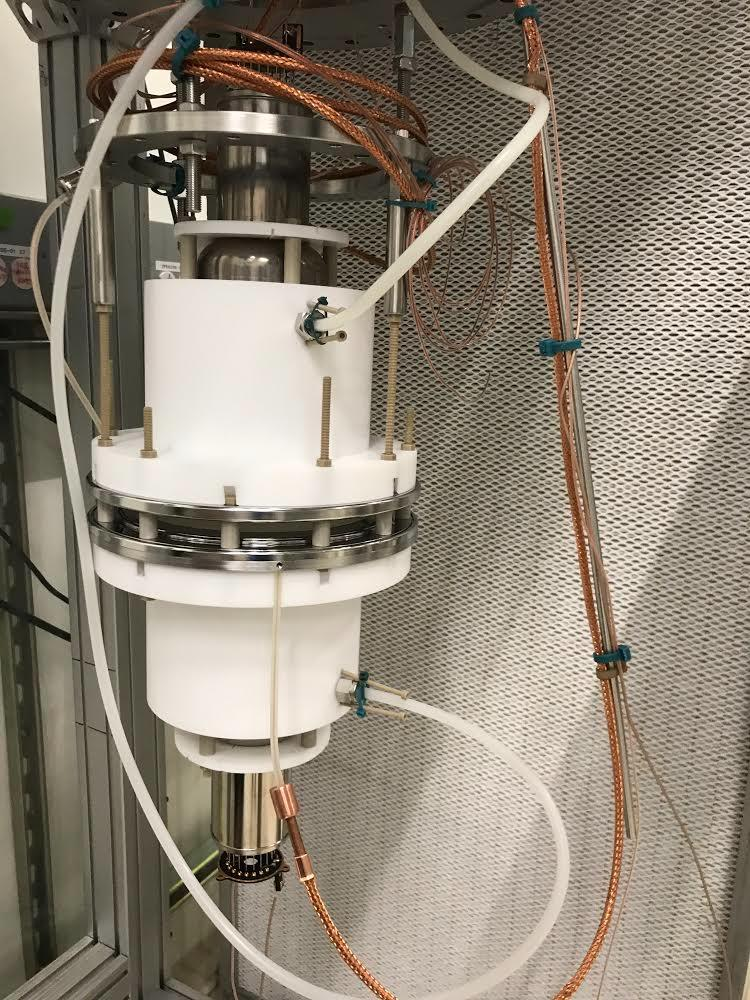
\includegraphics[width=\figurewidth,clip,trim={0 0 0 0},angle=0,origin=c]{Figures/GasTest/PhysicalLayout/GTGridTestRegion.jpg}
		\caption{}
		\label{fig:chambergeneral:gridtest}
	\end{subfigure}
	\begin{subfigure}[b]{\halfwidth}
		\centering
		\includegraphics[width=\figurewidth,clip,trim={0 0 0 0},angle=0,origin=c]{Figures/GasTest/PhysicalLayout/GTGasPanel.jpg}
		\caption{}
		\label{fig:chambergeneral:panel}
	\end{subfigure}
	\begin{subfigure}[b]{\halfwidth}
		\centering
		\includegraphics[width=\figurewidth,clip,trim={0 0 0 0},angle=0,origin=c]{Figures/GasTest/PhysicalLayout/GTBottles.jpg}
		\caption{}
		\label{fig:chambergeneral:bottles}
	\end{subfigure}
	\caption[\gtest\ apparatus physical layout.]{\gtest\ apparatus physical layout. (a) The \gtest\ detector: detector vessel (middle), electronic and gas gauge breakouts (top), Genie lift for detector assembly and disassembly (left), vacuum pumps and leak checking system (right). (b) ELD inside the detector vessel. (c) Gas circulation panel. (d) Circulation pump (left), and storage bottles (right). }
	\label{fig:chambergeneral}
\end{figure}

The electroluminescence detector (ELD) is the major location of active measurable electron emission events. Its conceptual drawing is illustrated in Fig.~\ref{fig:BasicELD}. A pair of grids for measurement are mounted in the center of the vessel. They are separated apart by 12 PEEK spacers, ,which are \SI{13}{\mm} in height. These two grids are biased to different voltages during the measurement. This creates a voltage difference between the two grids. It enables electrons between these two grids to produce EL photons ,which can be measured by the PMTs. The region between these two grids is called the EL region. 

\todo{These grids are named after their physical location in the detector as top grid and bottom grid. The grid plane diameters are \SI{140.9}{\mm} for the top grid and \SI{137.4}{\mm} for the bottom grid. Voltages of the two grids are noted as $V_{T}$ for the top grid and $V_{B}$ for the bottom grid. The voltage difference between the top and bottom grids is expressed with $\Delta V_{\text{T-B}}$ (dV) $\equiv V_{T} - V_{B}$. These grids also have another name by their bias voltages; the anodic grid and cathodic grid, and their voltage are respectively $V_{A}$ and $V_{C}$. The top grid is anodic and the bottom grid is cathodic when studying electron emission from the bottom grid, which is called normal polarity operation. Occasionally, the top grid is cathodic and the bottom grid is anodic when studying electron emission from the top grid, which is called reverse polarity operation. }

Two PTFE reflector cones are used to improve light collection efficiency for the primary scintillation and EL photons. These reflector cones are mounted on the top and bottom of the EL region. The surface of the PTFE cones overhang \SI{0.1}{mm} above the grid. The diameters of the opening of the PTFE cones to the grids are \SI{130}{mm}. The EL region have the most sensitivity for grid \ees\ with regart to light collection. The EL region defines the overall grid surface area of studying. Two PMTs mounted on the PTFE reflector cones are used to measure the primary scintillation and EL photons. Distances between the PMTs to the closest grids are \SI{110}{\mm}.

The two PMTs used to measure the primary scintillation and EL photons from events happening in the detector are model R11410-20 PMTs manufactured by Hamamatsu Photonics, as described in Ref.~\cite{HamamatsuPhotonics2006}. The model of PMT has a synthetic quartz window that is mostly transparent to incident photons of \SI{\sim 175}{\nm} (xenon scintillation photons). The PMT window is coated with a bialkali photocathode material, which absorbs the incident photon and emits electrons by the photoelectric effect. The emitted electron which lands on the effective area of the first dynode is multiplied along the PMT dynode chain in an electron gain process and observed, which is the measured signal.
The two PMTs are named after their physical location in the detector as top PMT and bottom(bot) PMT. Their spectral response of is summarized in Table~\ref{tab:PMTparameterHamamatsu}.
\begin{table}[!h]
	\centering
	\begin{tabular}[!tb]{ | m{16em} ||m{9em} | m{9em}| } 
		\hline
		&Top(top) PMT&Bottom(bot) PMT\\\hline\hline
		Serial Number & KB1163 & KB1170 \\\hline
		Cathode Luminous Sens. [\si{\uA\per\lumen}] & 149.0 & 148.0 \\\hline
		Anode Luminous Sens. [\si{\A\per\lumen}] & 657.0 & 1010.0 \\\hline
		Anode Dark Current [\si{\nA}] & 1.00 & 4.60 \\\hline
		Cathode Blue Sens. Index  & 12.60 & 12.30 \\\hline
		Q.E. [\si{\percent}] & &  \\\hline
		\quad \quad \SI{165}{\nm} & 22.1 & 21.2 \\\hline
		\quad \quad \SI{170}{\nm} & 33.3 & 32.6 \\\hline
		\quad \quad \SI{175}{\nm} & 36.3 & 36.0 \\\hline
		\quad \quad \SI{182}{\nm} & 37.1 & 37.0 \\\hline
		\quad \quad \SI{188}{\nm} & 36.1 & 36.2 \\\hline
		\quad \quad \SI{194}{\nm} & 33.9 & 34.1 \\\hline
		\quad \quad \SI{200}{\nm}& 32.6 & 32.9 \\\hline	
	\end{tabular}
	\caption[Spectral response of PMTs tested at Hamamatsu Photonics]{Spectral response of PMTs tested at Hamamatsu Photonics.}
	\label{tab:PMTparameterHamamatsu}  
\end{table}

A CAEN R1470ETD high voltage power supply is used to bias the two grids and the two PMTs. Two custom ceramic feed-throughs are used to deliver high voltage to the two grids in the detector vessel. Each feed-through has a low-pass filter box attached for noise removal. Custom designed cables and cable terminations are used to apply voltages through the feed-throughs to the grids. The cable terminations were a limitation on our ability to bias the grids to high voltage. New design elements have been introduced to solve this problem. Details of iterations of these designs will be discussed in Chapter.~\ref{chap:gtestresult}.    

\begin{figure}[!tb]
\centering
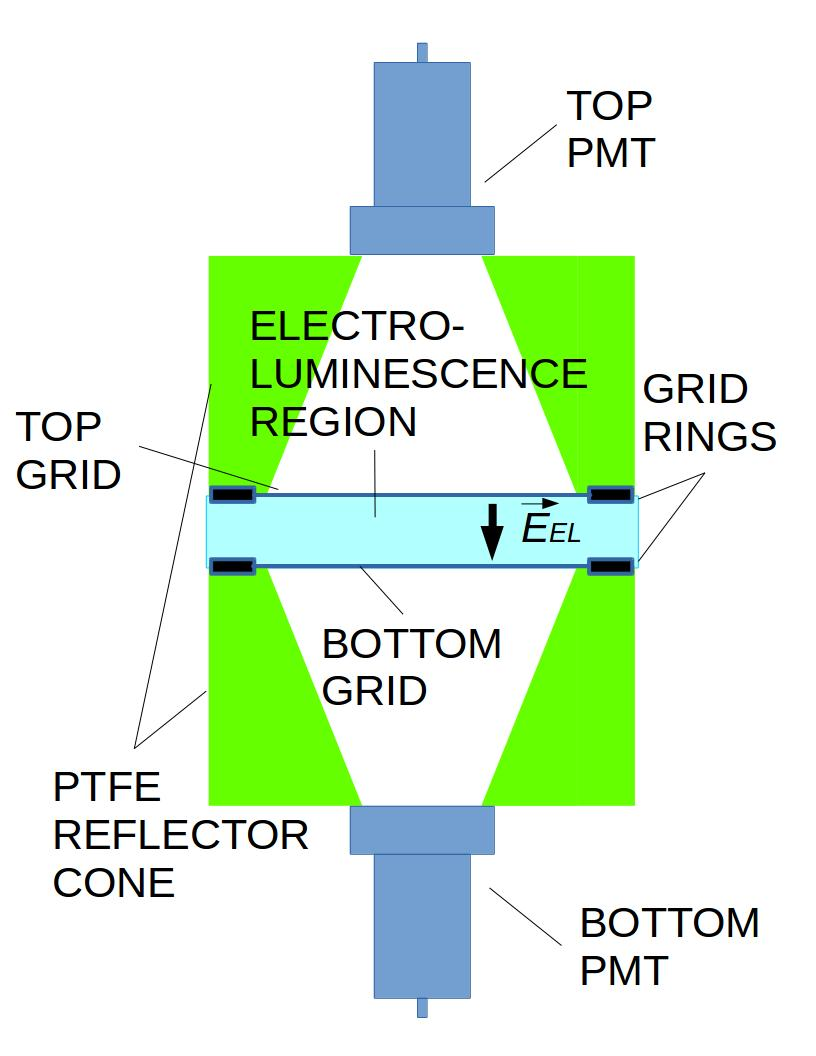
\includegraphics[width=\halfwidth,clip,trim={0 0 0 0},angle=0,origin=c]{Figures/GasTest/WeiDrawEvent/BasicELD.jpg}
\caption[\gtest\ electroluminescence detector.]{Conceptual drawing of \gtest\ electroluminescence detector (ELD)}
\label{fig:BasicELD}
\end{figure}

\paragraph{Gas circulation system}
A gas circulation system is used to purify, add, and remove xenon gas in the detector. The circulation system %panel is designed for continuous purification of noble gas element in the detector. This
maintains the gas purity condition in the detector, which is essential for the operation for the following reasons. %It removes impurity atoms such as oxygen, water, and hydrocarbons. 
The purity of xenon gas ensures that electrons that are produced in the ELD do not combine with impurity atoms, thus decreasing the production of primary scintillation and EL light. The purity of xenon also has a notable effect on electron drift velocity in xenon gas, which biases our study; that is impure xenon gas tends to have a slower electron drift velocity. The deviation of electron drift velocity between different impurity levels can reach \SI{20}{\percent} in certain reduced electric fields (ratio of electric field to gas density), as described in Ref.~\cite{Brooks1982}. This deviation biases the \ees\ selection, which is based on the predicted pulse duration according to electron drift velocity, and introduces systematic error to the \ees\ study.

Xenon purification is carried out with the following elements in the gas circulation system. A gas circulation panel (Fig.~\ref{fig:chambergeneral:panel}) is used to control the flow of xenon gas. A SAES PS3-MT3-R-1 rare gas purifier getter mounted on the circulation panel is used to purify the gas. The getter element has a sub-ppb efficiency of removing water, nitrogen, oxygen, carbon oxide, carbon dioxide, hydrogen, and hydrocarbons%. The capacity of the getter is more than \todo{\SI{0.1}{\meter\cubed}} in volume of nitrogen and oxygen. 
%With continuous purification, noble xenon gas achieves a purity of nitrogen, oxygen and water contamination better than \SI{1}{\ppb}
, as described in Ref.~\cite{SAESgetters2002}.  A custom pump (Fig.~\ref{fig:chambergeneral:bottles}) manufactured by KNF Neuberger, Inc. drives the gas circulation in the system. This pump is a type PM26101-0150.1.2.12 double diaphragm pump, which has company specified \SI{1.5}{\bar} operating pressure, as described in Ref.~\cite{KNFNeuberger}. During the actual operation, the pump works at pressures of up to \SI{3.7}{\bar} with a leak rate less than \SI{e-7}{\bar\liter\per\s}. An Alicat MC-5SLPM-D-485 mass flow controller (MFC) on the gas circulation panel controls the circulation flow rate, which allows a maximum flow rate of \SI{5}{\slpm}, as described in Ref.~\cite{AlicatScientific}. During the gas purification process, the flow of gas was controlled and driven through the getter for \SI{\sim 20}{\min} to allow the complete absorption of the gas impurities in the detector. This process is frequently conducted between each dataset to ensure the gas purity quality. 

The addition and removal of xenon gas are carried out with the same gas panel. Two \SI{4}{\liter} bottles (Fig.~\ref{fig:chambergeneral:bottles}) are used for the storage of xenon gas used in the tests when the gas is not used in the detector. During the xenon gas removal process, these bottles are inserted into two dewars filled with liquid nitrogen. Reducing the temperature of the bottles by using liquid nitrogen allows xenon gas to flow through the gas circulation panel back to the bottles, and to condense inside the bottles. During the addition of xenon gas process, the bottles are taken out from the dewar and warmed up. This process raises the gas pressure in the bottle, which drives the gas to fill the detector through the getter on the gas panel. The gas flow is controlled by the gas regulator and the MFC on the panel.   

\section{Data Acquisition} %f1
\label{sec:gtest daq}
A data acquisition(DAQ) system is used for recording PMT pulses for grid emission tests. The DAQ system is designed and made at \slac , previously used and tested in \phaseone\ detector. The DAQ system is customized to maximize the probability for capturing single photon electron (\sphe ) pulses from the PMTs. This also enables the DAQ system to record \ees s, which are collections of multiple \sphe\ pulses. The DAQ system contains three parts: (1) amplification and digitization, (2) recording, and (3) transfer and storage. The DAQ system works continuously, except when interrupted by the data transfer process. This interruption is called dead time of the DAQ system. The dead time issue %in studies of \ees s 
is addressed by the subtraction of live times after each recorded pulses. Aspects of the DAQ system are described below. %This set the limit of speed for DAQ.

\paragraph{Amplification and digitization} %f1
%purpose
This process amplifies and digitizes PMT pulse signals. The amplification and digitization of the PMT signals are carried out by two separate custom made boards. The amplification of signals improves signal to noise ratio. %This eases background signal selections. 
However, this amplification may also cause distortion of the waveform if the pulse signal amplitude exceeds the maximum capability of the electronic circuits in the amplification and digitization boards. Two amplifier gain settings are implemented: low gain ($\times$ 12), and high gain ($\times$ 100). For electron emission tests, the low gain setting is used to obtain a satisfactory signal to noise ratio. The low gain setting allows \numrange{40}{60} \sphe s to be recorded simultaneously without distortion, when the high gain setting is not used because its without distortion \sphe\ recording range is only \numrange{5}{7} \sphe s, which is too small for the counts of simultaneous \sphe s in \ees s.
An optical fiber connecting these two boards transfers the amplified PMT signals to the digitizer board. The digitizer board is capable of doing a \SI{16}{\bit} digitization in a dynamic range of \SI{2.5}{\V} (\SIrange{\sim -1.26}{1.24}{\V}). The digitizer reverses the polarity of signals, which changes \sphe\ pulses from negative spikes to positive spikes. The digitizing sampling frequency is every \SI{4}{\ns}. Digitized data are written to a buffer memory in the digitizer board. %This writing happens continuously, except for interrupted by data transfer. This is called dead time of DAQ, and will be explained below. 
The amplification and digitization system sets the precision of \sphe\ measurement and signal to noise ratio, and digitizes PMT pulse signals to be handled numerically later.
%Fig.~\ref{fig:DAQPhysicalLayout} shows DAQ system physical layout.

\begin{comment}

\begin{figure}[!tb]
 \centering
 \begin{subfigure}[t]{\halfwidth}
    	    	\centering
   \includegraphics[height=15em]{Figures/GasTest/PhysicalLayout/PreAmp.jpg}
   \caption{}
   \label{fig:amplifier}
 \end{subfigure}
 \begin{subfigure}[t]{\halfwidth}
    	    	\centering
   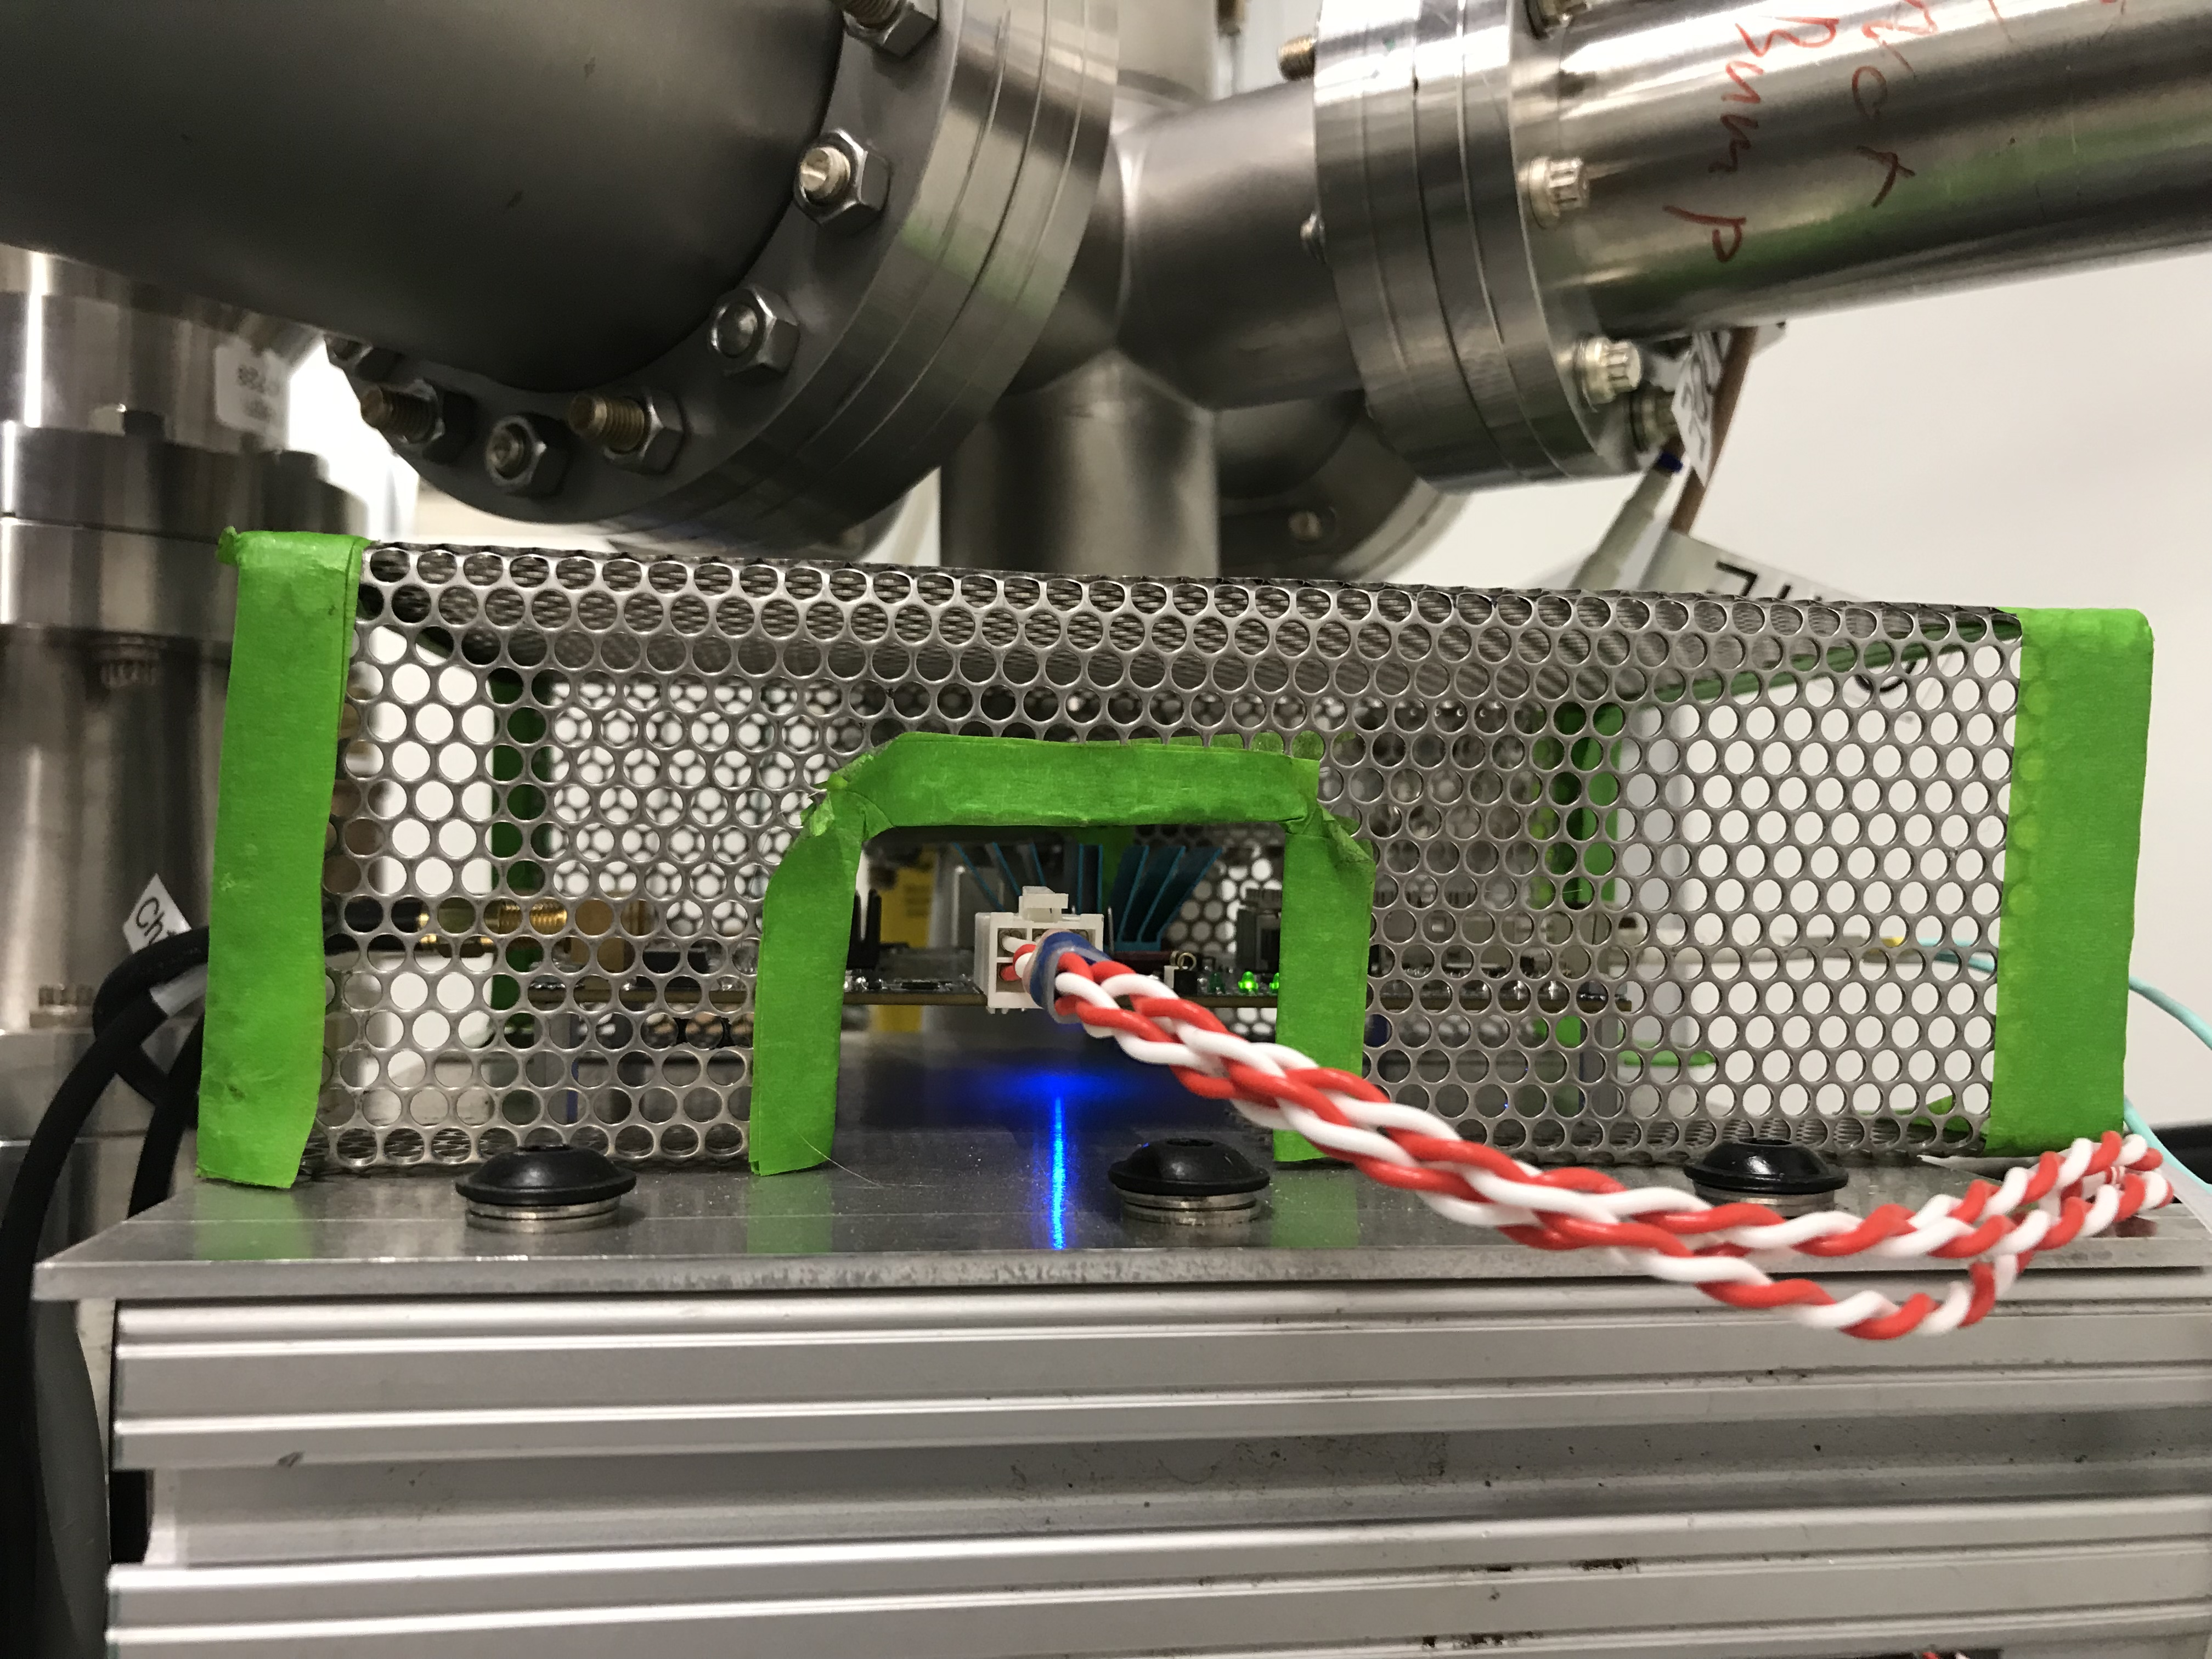
\includegraphics[height=15em]{Figures/GasTest/PhysicalLayout/DigitizerInBox.jpg}
   \caption{}
   \label{fig:digitizer}
 \end{subfigure}
 \caption[\gtest\ data acquisition system physical layout.]{\gtest\ data acquisition system physical layout: (a) amplifier board. (b) digitizer board.}
 \label{fig:DAQPhysicalLayout}
\end{figure}
	
\end{comment}

\paragraph{Recording} %f1 
The recording system for DAQ makes decisions for data recording. The decision making algorithm is controlled by customized DAQ XML parameters in an XML file. The pulse recording is undertaken in a pending mode without a conventional trigger, which is explained below. First, the continuous digitized pulse amplitude data are compared to a pre-threshold voltage (trigger voltage), which is called the pre-threshold value, until a threshold crossing is reached. The time of this threshold crossing is the pulse recording reference time (trigger time). Pulse recording also includes a preceding segment of samples, which is called the pre-delay. The start time of the pre-delay period is the pulse recording start time. Next, digitized data are compared to a post-threshold voltage, which is called the post-threshold value, until a threshold crossing is reached. Then, the pulse recording continues for a succeeding segment of samples, which is called the post-delay. During the post-delay period, the digitized data are compared to the pre-threshold value again. If no pre-threshold crossing is reached, the pulse recording ends when the post-delay period ends. Otherwise, the DAQ system keeps recording until after a post-threshold crossing is reached, no other pre-threshold crossing is reached in the next post-delay period. The end time of the last post-delay period is the pulse recording stop time. The pre-threshold values are chosen so that the \sphe\ recording efficiency, also called the trigger efficiency, of both PMTs are larger than \SI{95}{\percent}. The trigger efficiency is estimated by fitting \sphe\ amplitude distributions to Gaussian distributions, as described in Section~\ref{sec:pmt cal}. Results of these evaluations show that at normal PMT operating voltage (\SI{-1.5}{\kV}) the top PMT and the bottom PMT have good trigger efficiency of \SI{99.6}{\percent} and \SI{>99.9}{\percent}. The recorded pulses are called pulses of digitization (PODs), which are one of the fundamental elements for the next step; coinciding event building, as described in Section~\ref{sec:gtest data process}.

The used DAQ XML parameters during the tests are summarized in Table~\ref{tab:DAQparameters}.

\begin{table}[!h]
  	\centering
 \begin{tabular}[!h]{ | m{7em} ||m{7em} | m{5em}| m{15em}| } 
   \hline
   name & XML parameter name & value & explanation \\\hline\hline 
   post-delay & `PostDelay' &  \SI{500}{\sample} &counts of samples to keep after crossing post-trigger threshold ('PostThreshold'). \\\hline
   pre-delay & `PreDelay' &  \SI{30}{\sample}& counts of samples to keep before crossing pre-trigger threshold ('PreThreshold'). \\\hline
   post-threshold & `PostThreshold' & 0x7D80 or as needed &  crossing this threshold value determines the stop time of pulse recording.\\\hline
   pre-threshold & `PreThreshold' & 0x7D61 or as needed & crossing this threshold value determines the start time of pulse recording.\\\hline
 \end{tabular}
 %\begin{flushright}    	
 %\end{flushright}
   \caption[Data Acquisition system parameters.]{DAQ system parameters. (\SI{1}{sample} is \SI{4}{\ns}.) }
   \label{tab:DAQparameters}
\end{table}

\paragraph{Transfer and storage} %f1
The transfer and storage system transfers data from the digitizer board and stores data in binary format in the main computer system. The buffer memory data that pass the selection of trigger algorithm are transferred through an optical fiber and written to files stored in the main computer. The data transfer speed is \SI{250}{\mega\byte\per\second}. For an average pulse duration of \SI{2}{\us} (\SI{500}{\sample}), the DAQ allows approximately 30 thousand pulses to be recorded per second. The continuously recorded data are separately saved to series of files; each with a maximum size of \SI{1.1}{\giga\byte}. The process of data transfer interrupts the process of buffer memory writing of the incoming digitized data, which raises the dead time issue. 

\paragraph{Dead time} %f1
The dead time of DAQ is the segment of time that the DAQ system stops working after the end of each pulse recording. The reason for the dead time is because the process of buffer writing and the process of data transfer in the DAQ system cannot happen simultaneously. Dead time issue brings challenges in measuring electron emission rates. 
%Dead time seems to occur in each PMT channel independently from each other. 
The duration of dead time shows a dependence on the preceding pulse duration. However, the quantitative relationship between the two is unclear. We address this issue by subtracting a segment of time succeeding each recorded pulse from the live time of study.  

We studied the dead time issue by using two methods. The first method is finding problematic pulses that might be a result of dead time. We found there exist a population of pulses that when one PMT detects large quantities of photons, the other PMT detects no photon simultaneously. Since the two PMTs are observing the same space in the ELD, we expect to see similar magnitude of photons in both PMTs. The most likely reason for this to happen is that the other PMT channel is suffering from dead time. The other possible causes of these problematic pulses, such as misbehavior of one PMT, are less dominant. The time difference between the recording time of large quantities of photons in one PMT and the first preceding pulse in the dead time problematic PMT is the potential duration of dead time, as shown in Fig.~\ref{fig:pulse dead time}. 
More than \num{400} dead time problematic pulses are examined. From the examinations, we found that for a particular pulse with a duration of \SI{2}{\us}, the duration of dead time is in the range of \SIrange{0.3}{15}{\us}. For longer pulses, we observe the duration of dead time for as long as \SI{80}{\us}.

\begin{comment}
	\begin{figure}[!p]
	\centering
	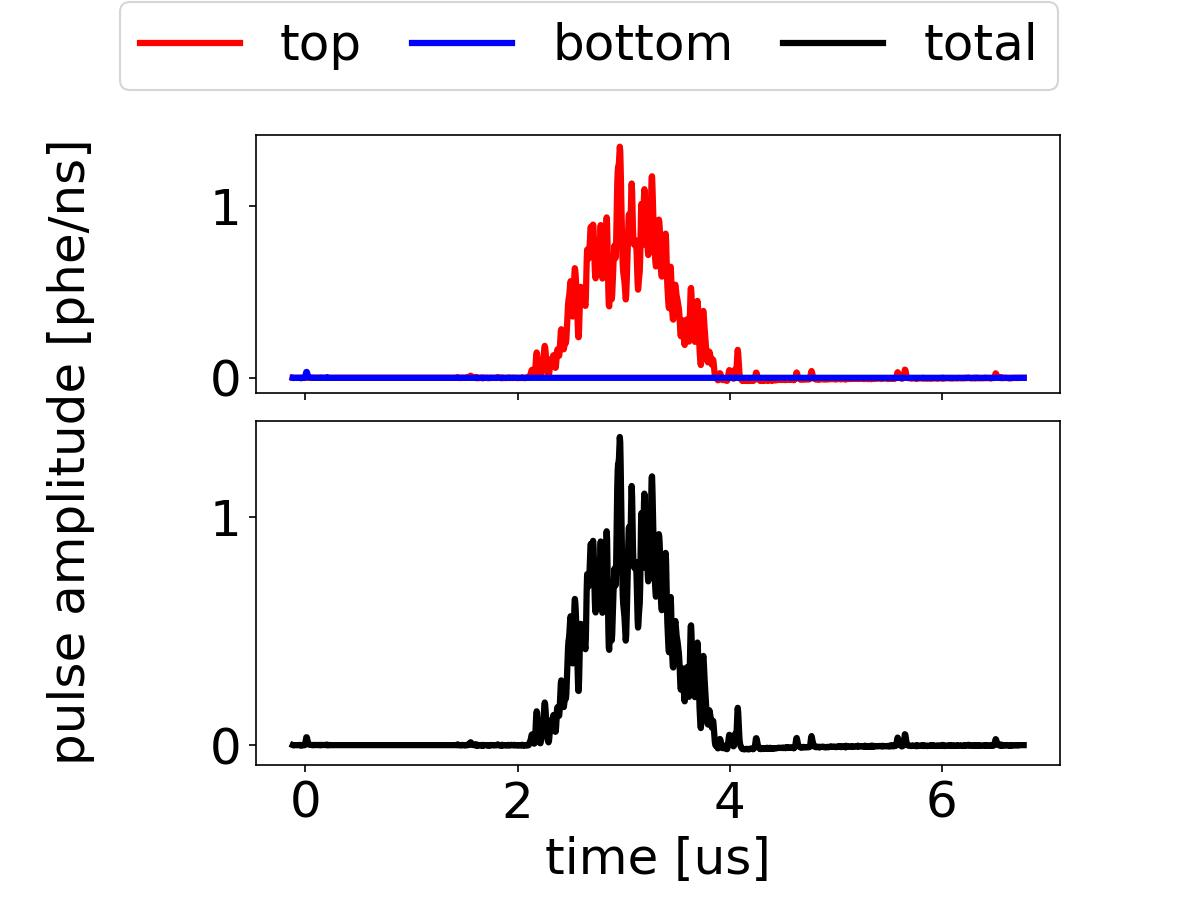
\includegraphics[width=\figurewidth,clip,trim={0 0 0 0}]{Figures/GasTest/exampleWaveforms/proc64767id00000065.jpg}%{Figures/GasTest/CutsValid/wave/testproc65831coinid0.jpg}
	\caption[\gtest\ signal: an example waveform during dead time.]{\gtest\ signal: an example waveform during dead time.}
	\label{fig:pulse dead time}
\end{figure}
\end{comment}

\begin{figure}
	\centering
	\begin{subfigure}[b]{0.8\textwidth}
		\centering
		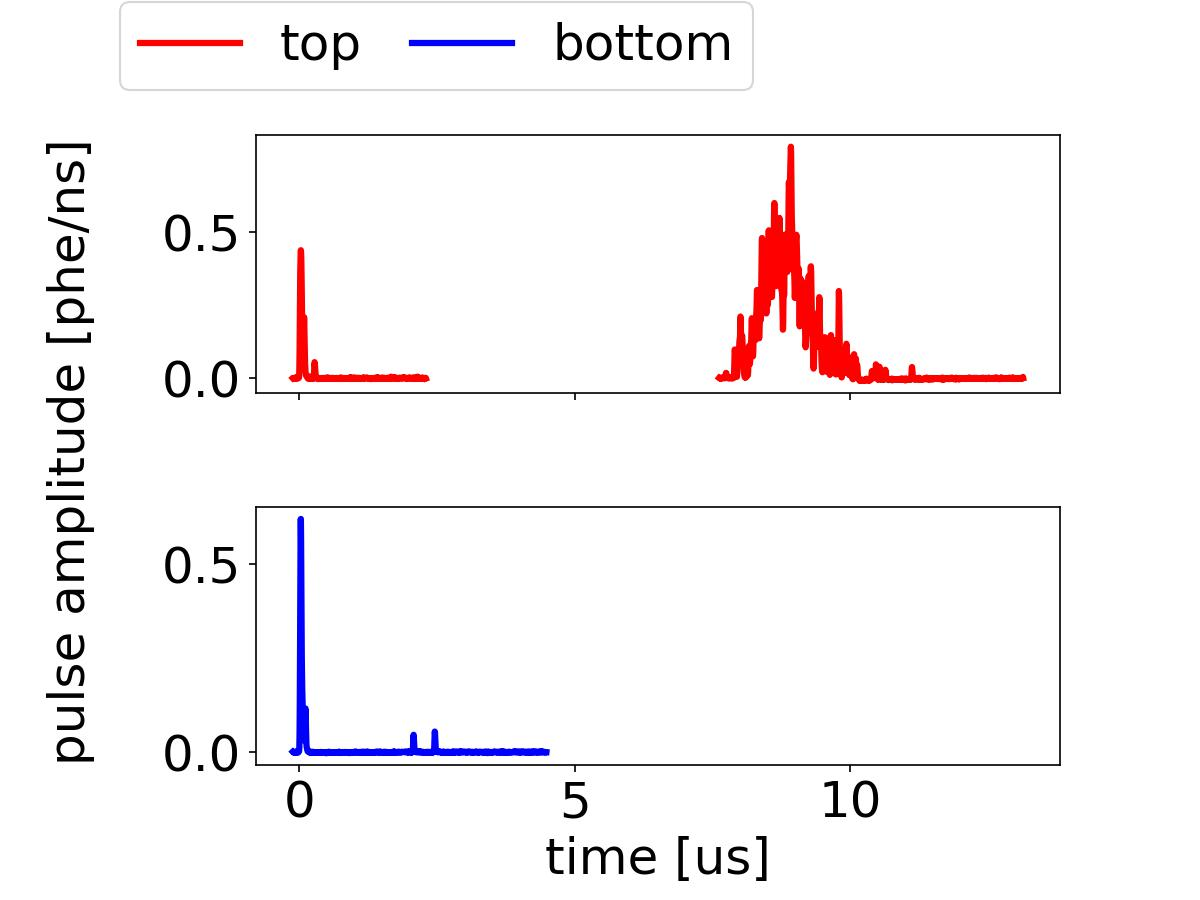
\includegraphics[width=\figurewidth,clip,trim={0 0 0 0}]{Figures/GasTest/exampleWaveforms/proc64767DeadTime1.jpg}
		\caption{}
		\label{fig:ptfe fluo c}
	\end{subfigure}
	\par\bigskip
	\begin{subfigure}[b]{0.8\textwidth}
		\centering
		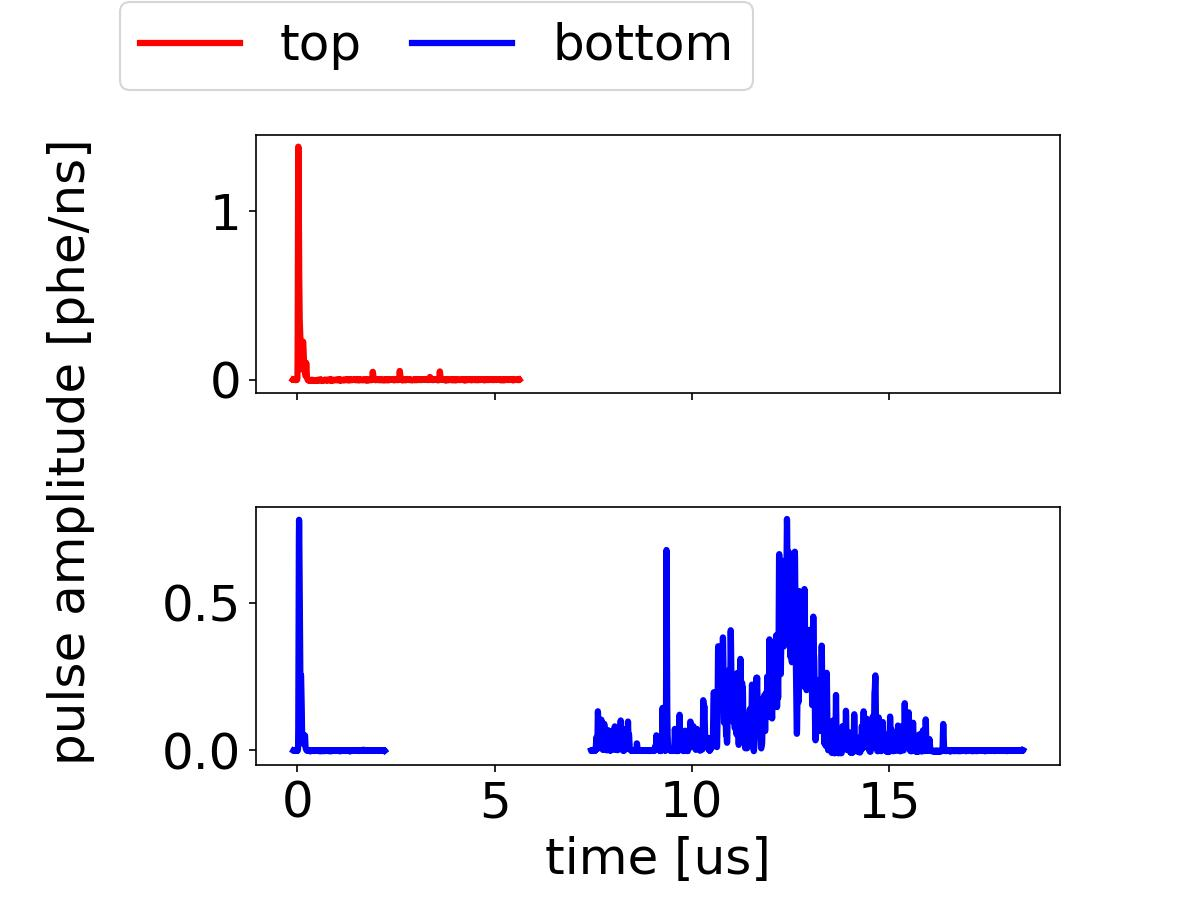
\includegraphics[width=\figurewidth,clip,trim={0 0 0 0}]{Figures/GasTest/exampleWaveforms/proc64767DeadTime2.jpg}
		\caption{}
		\label{fig:ptfe fluo d}
	\end{subfigure}
	\caption[\gtest\ signal: example waveforms during dead time.]{\gtest\ signal: example waveforms during dead time. (a) The top PMT channel is suffering from dead time. (b) The bottom PMT channel is suffering from dead time. }

	\label{fig:pulse dead time}
\end{figure}

%The second method is finding the probability difference of the pulse recording stop time and the pulse recording start time of two sequentially recorded pulses between pulses recorded by one PMT and pulsed assuming uniform time distribution, which should mimic the case with no dead time issue. 
To estimate the systematic error, we employ a second method based on the idea that the presence of dead time will shift the distribution of time intervals between two consequential pulses in one PMT. In the absence of dead time, the time distribution should be an exponential distribution characterized by the average rate, which is expressed by: %The impact of dead time is to shift time difference probability an exponential curve, which is from assuming uniform distribution:
\begin{align}
	\text{probability} = \frac{1}{\tau}\exp \left( - \frac{t}{\tau} \right)
\end{align}
where $\tau$ is the time constant, which is the inverse of the average rate. 

Results of this shift are shown in Fig.~\ref{fig:PMTdeadtime}. %The figure shows the best fit exponential curve of two sequentially recorded pulses time differences in one PMT that have such time difference larger than \SI{100}{\us}. 
%This fitted curve better reflects the distribution of no dead time issue case by subtracting the potential duration of dead time. 
%The difference between the fit curve and the data reflects the influence of the duration of dead time, which indicates the dead time issue is subdominant after \SI{20}{\us}.  
The figure includes studies of pulses categorized by their durations. These studies confirm the previous conclusion about the dead time issue and further show that the dead time duration is dependent on the preceding pulse duration. The low statistics at the small time interval range, e.g. range \SIrange{0}{e2}{\us} for pulse length in the range of larger than \SI{30}{\us}, clearly show the shift from the expected exponential distribution. The low statistic region varies with the preceding pulse duration, as summarized in Table~\ref{tab:PMT dead time duration}. The difference on the slopes of these curves is due to PTFE fluorescence that occurs subsequent to each pulse, which is more obvious for larger-area (long-duration) pulses, and increases the average rate succeeding such pulses, as will be discussed in Section~\ref{sec:events}. 

\begin{figure}[!p]
	\centering
	\begin{subfigure}[t]{\twofigurewidth}
		\centering
		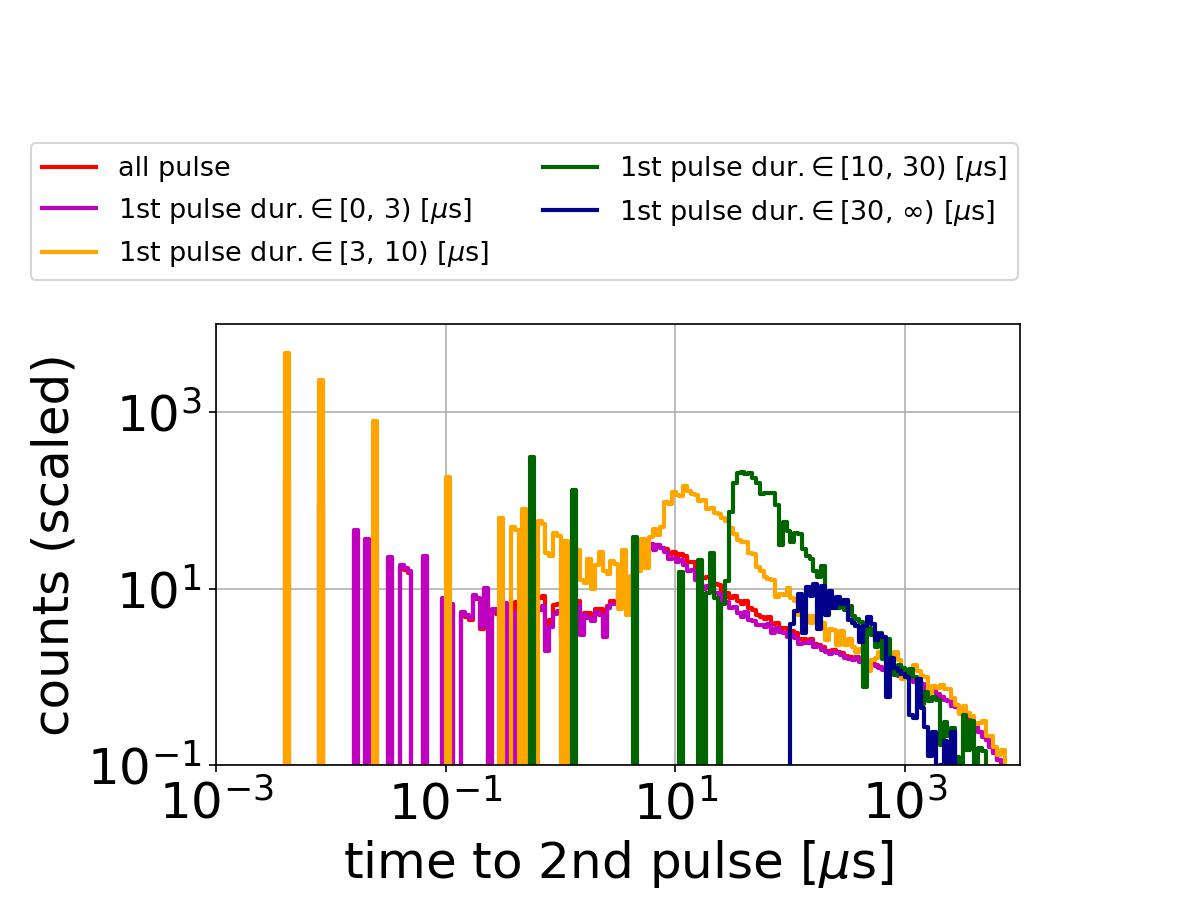
\includegraphics[width=\textwidth,clip,trim={0 0 0 0},angle=0,origin=c]{Figures/GasTest/DatasetQuality/topPMTdeadtime64767.jpg}
		\caption{}
		\label{fig:PMTdeadtime top}
	\end{subfigure}
	\begin{subfigure}[t]{\twofigurewidth}
		\centering
		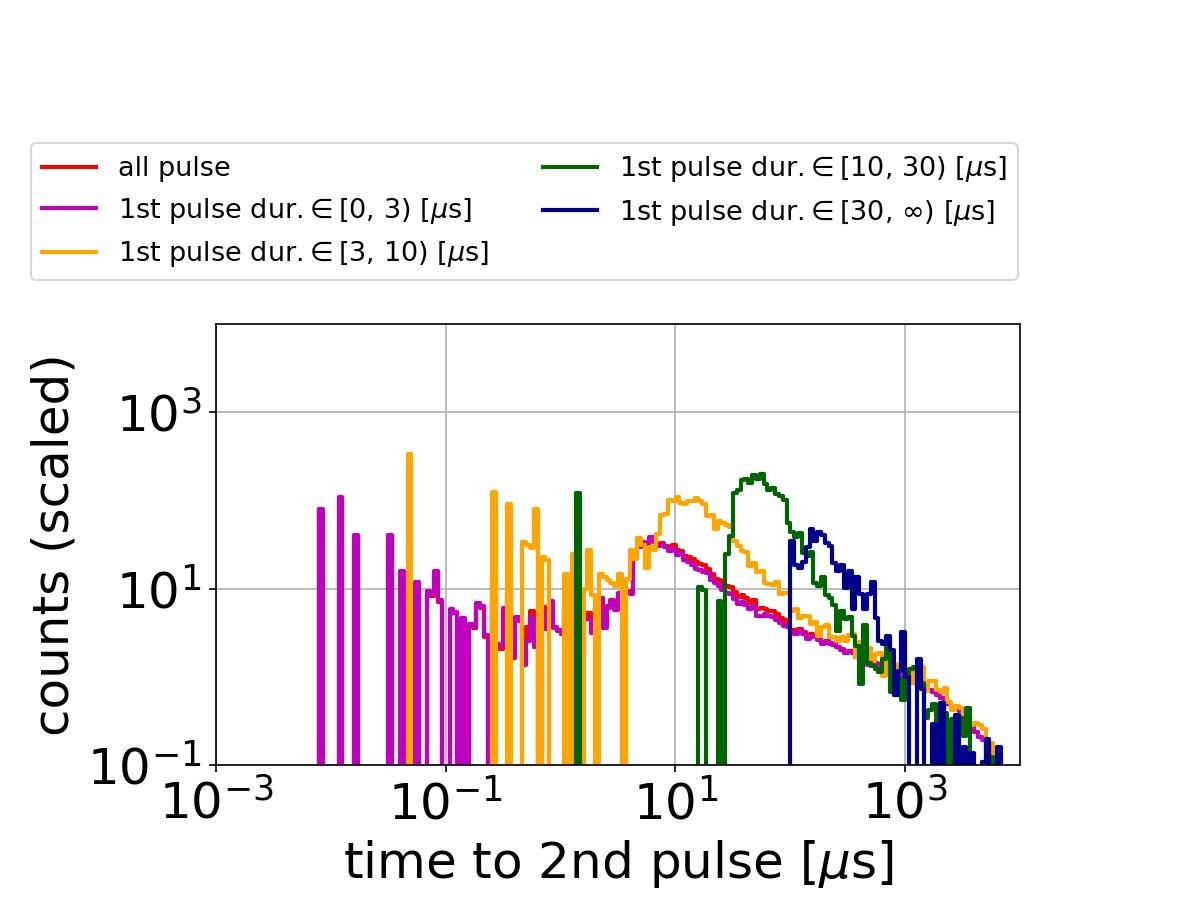
\includegraphics[width=\textwidth,clip,trim={0 0 0 0}]{Figures/GasTest/DatasetQuality/botPMTdeadtime64767.jpg}
		\caption{}
		\label{fig:PMTdeadtime bottom}
	\end{subfigure}
	\caption[Distribution of PMT time differences between pulses in one PMT.]{Distribution of PMT time differences between pulses in one PMT: (a) top PMT; (b) bottom PMT. }
	\label{fig:PMTdeadtime}
\end{figure}

	\begin{table}[!h]
		\centering
		\begin{tabular}[!h]{| m{11em} ||m{11em} | m{11em}| } 
			\hline  pulse duration & dead time duration & dead time duration \\
			  & (low statistics region) & (maximum observed) \\
			 $\text{[\si{\us}]}$  & $\text{[\si{\us}]}$ & $\text{[\si{\us}]}$ \\\hline\hline
			  all & 7 & 80 \\\hline
			  [0, 3) & 7 &  15 \\\hline
			  [3, 10) & 10 &  15 \\\hline
			  [10, 30) & 50 &  80 \\\hline
			  [30, $\infty$) & 100 &  80 %\\\cline{2-4} 
			\\\hline
		\end{tabular}

		\caption[PMT dead time duration]{PMT dead time duration.  Data were taken at \ddtt{2017}{12}{08}{14}{02}, with \opvtvb\ at \SIlist{+6;-6}{kV}, \opgd\ at \standarddensity .}
		\label{tab:PMT dead time duration}
	\end{table}

Thus, to resolve the dead time issue, we subtract a segment of time after each recorded pulse from the live time of study and eliminate all pulses that are recorded in this time period, as described in Section~\ref{sec:cuts}. The remaining pulses are used to study the absolute rate of signals of interest; \ees s. The rate of signals of interest is close to the absolute rate without the dead time issue from the view of DAQ behavior.

\section{Operation} %f1

%\todo{think about where to put run selection section. I want to take about , what is sparking test, what is normal operation before electron emission tests. This is the reason this section is here. however, put it just in front of cut might also be good.}

We make sure to have stabilized operation conditions to study the electron emission process from grids. This allows us to obtain results at a fixed condition and to compare results between different operations.  %It makes it possible for us to compare results between different runs. 

\paragraph{Operating conditions} %f1
When running the \gtest\ electron emission tests, (1) the detector is filled with xenon gas, (2) two PMTs are running stably, and (3) two grids are biased to proper voltages. 

The typical operating xenon gas density for the electron emission tests is \SI{0.137}{\mole\per\liter}  (\SI{\sim 3.3}{\bara} at temperature \SI{295}{\kelvin}, or equivalent to the xenon gas density at \SI{177}{\kelvin} on xenon liquid-vapor saturation curve). 
This choice minimizes the probability of discharges between the two grid electrodes. %It also makes the grids operate under the gas density closest to \lze\ operating gas density. 
These discharges may cause potential damage to grids, and also prevent stable running of the tests. 

The gas operating condition at a density of \SI{0.137}{\mole\per\liter} allows us to measure the electron emissions in the sensitivity range of \opdv\ \SIrange{8}{16}{\kV}. The grids that we use in our tests are usually woven with a wire diameter of  \SI{75}{\um} and a distance between two parallel wires of \SI{5}{mm}. For these grids, the sensitivity \opdv\ range corresponds to an average \wsef\ in the range of \SIrange{65}{110}{\kV\per\cm}. However, since EL production decreases as the reduced electric field (ratio of electric field to gas density) in the EL region decreases, the photon production per electron emission is smaller for a lower \opdv . This prevents us from having enough sensitivity to study the electron emission for a lower operating voltage and \wsef . So the electron emission rate for a lower \wsef\ is measured at a lower gas density to get an increase of the reduced electric field, which leads to a higher EL photon production in gas. The dependence of the EL light production on reduced electric field is described in Section~\ref{sec:events}.

Two PMTs normally operate at \SI{-1.5}{\kV}. This guarantees that both PMTs have enough gain and signal to noise ratio. Before safely turning on the PMTs to measure the light from electron emissions from the grids, a series of tests are conducted to figure out the high voltage behavior and high voltage weak points in the system. Improvements are made to increase the maximum \opvtvb\ ,under which the two grids do not create discharges. These improvements include cleaning the surface of spots which create discharges, increasing the smoothness and the rounding radius on the corner of metal surfaces, and increasing the distance between the electrodes and the ground. Physical contact with the grid wires is avoided during these improvements. The maximum \opvtvb\ that these grids can hold without creating discharges are measured with different gas (e.g. xenon, argon, and nitrogen) and different pressures. The dark current \sphe\ rate of both PMTs while they are stable running is approximately \SIrange{0.500}{1}{\kHz}. Test which produce a \sphe\ rate above \SI{2.5}{\kHz} are excluded. 

The high voltage power supply is capable in biasing both grids separately in the range of \SIrange{-8}{8}{\kV}. The current between the power supply and the grid is monitored to guarantee stable operation of grid bias voltages. An unstable grid biasing usually shows as a spike in the monitored current, and a spike on PMT recording rates. These segments of time referring to the unstable current are excluded.  

\paragraph{Obtaining data} %f1
The most common operating voltages we choose for electron emission measurements are $V_{T}=-V_{B} $ at \SIlist{\pm 4; \pm 4.5; \pm 5; \pm 5.5;\pm 6; \pm 6.5;\pm 7; \pm 7.5;\pm 8}{\kV}. This voltage range allows us to measure the electron emission rate vs. \opdv\ for most grids we study. Measurements outside this voltage range are also performed to understand the detector better. However, their results usually are not included in the electron emission studies.

The typical duration for obtaining data is three minutes. An increasing trend of light production is seen during the operations when obtaining data takes longer than three minutes. This is probably from the increase of EL light production in the more ionized chamber environment and the increase of fluorescence light emissions from the PTFE reflector cones in the detector. Usually, after each \SI{3}{\min} dataset, high voltage power for both grids are set back to \SI{0}{\kV} and rest for at least \SI{30}{\s} before the next measurement is taken. Obtaining data at each voltage configuration is handled by using scripts in Ignition slow control software, as described in Ref.~\cite{Ignition2018}. This is to make sure obtaining data is consistent and reproducible.

Datasets with the cathodic grid bias voltage \SI{> -2.5}{\kV} are explicitly excluded from electron emission measurements. The reason is because this configuration allows electrons created by external particles in the cone region to drift to the EL region. These electrons will produce EL light in the EL region, the process of which could introduce a background rate for the electron emission studies. The process is illustrated in Fig.~\ref{fig:BelowCathodeIllustration}.

\begin{figure}[!p]
 \centering
 \begin{subfigure}[b]{\halfwidth}
 			\centering
   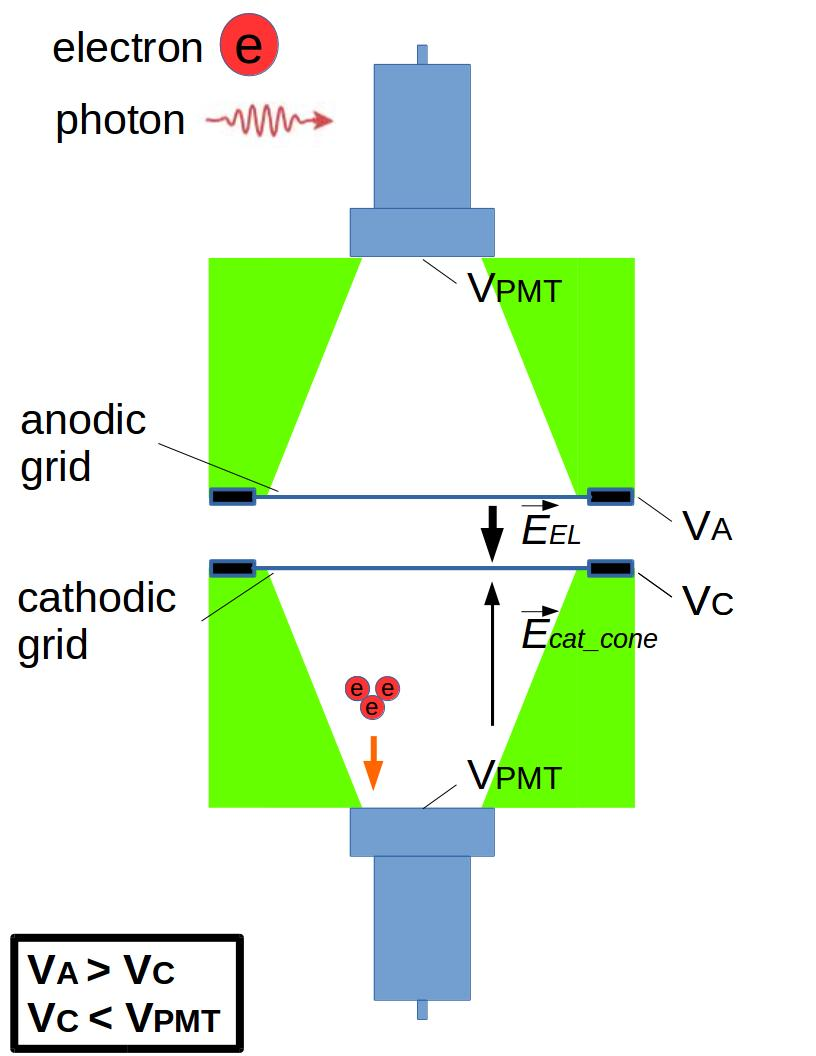
\includegraphics[width=\figurewidth,clip,trim={0 0 0 0},angle=0,origin=c]{Figures/GasTest/WeiDrawEvent/GoodConfig.jpg}
   \caption{}
   \label{fig:BelowCathodeIllustration:GoodConfig}
 \end{subfigure}
 \begin{subfigure}[b]{\halfwidth}
 			\centering
   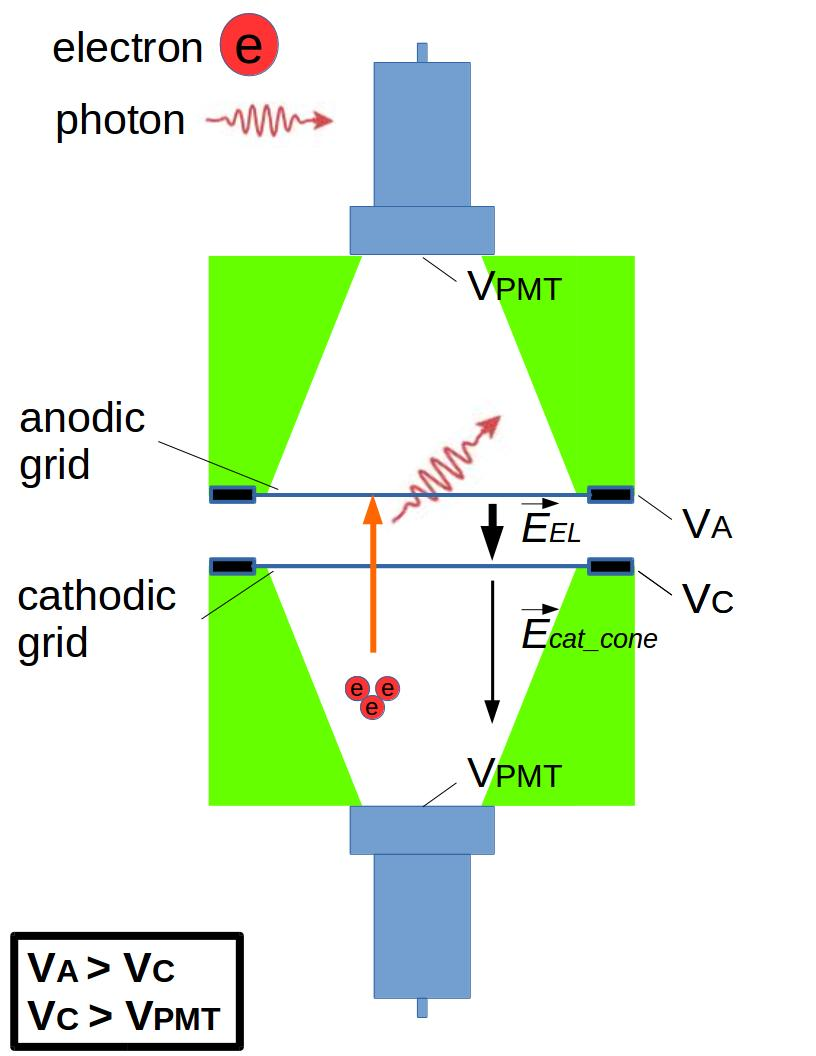
\includegraphics[width=\figurewidth,clip,trim={0 0 0 0}]{Figures/GasTest/WeiDrawEvent/BadConfig.jpg}
   \caption{}
   \label{fig:BelowCathodeIllustration:BadConfig}
 \end{subfigure}
 \caption[\gtest\ good and bad voltage configurations.]{(a) Good configuration ($V_{C} < V_{PMT}$): drift fields pointing from PMT to the grids. Electrons created in the cone region will drift to PMT. This process does not create numerous photons as \ees . (b) Bad configuration  ($V_{C} > V_{PMT}$): drift fields pointing from grids to the PMT. Electrons created in the cone region will drift to EL region. This process creates plenty of EL photons which could look like an \ees .}
 \label{fig:BelowCathodeIllustration}
\end{figure}

\section{Data processing} %f1
\label{sec:gtest data process}
Data processing is undertaken to save the useful information from the data by reducing the amount of extraneous information. %This reduces size of analysis works. 
The useful information of a pulse are characterized by Reduce Quantities (RQs) of a pulse.

The data processing framework includes three parts: (1) single pulse processing, (2) coinciding event building and coinciding pulse processing, and (3) random segment sampling of the dataset.

This section explains the main part of the data processing framework. It does not seek to explain all the RQs that have been computed. A full documentation of the RQs used in \gtest\ analysis is summarized in Appendix~\ref{chapter:gastestRQ}.

\paragraph{Single pulse processing} A single pulse of digitization, POD, is defined to be the individual pulse recorded by the DAQ system in only one PMT channel. This processing requires two steps: (1) waveform reconstruction, and (2) pulse shape characterization. 

The waveform is reconstructed by the following method. First, the baseline voltage of the pulse (RQ name: `baselines') is identified based on the average DC voltages of the pulse of the first 10 samples. The baseline voltage represents the voltage at the time when the pulse is recorded, assuming no pulse occurs. Samples used for identifying the baseline voltages are \SI{80}{\ns} ahead of the trigger time of the pulse. Therefore, these samples provide a reliable measure of the baseline as they are close in time from and unaffected by the rest of the pulses. %In principle, baseline voltages are not effected by the succeeding pulses. Thus, they reflects DAQ quiet bias voltages. 
There are certain fluctuations of baseline voltages for both PMTs. The amplitude of fluctuation \SI{\sim 0.36}{\mV} is very small compared to the average \sphe\ pulse amplitude, which is \SIrange{15}{35}{\mV}. After identifying the baseline, the baseline value was subtracted from the digitized data to get the waveform of the pulse. The waveform is then scaled back from ADC counts to \si{\mV} to get the reconstructed waveforms. Along this process, RQs for the voltage of the trigger sample (RQ name: `trigvals'), and the voltage of the first sample (RQ name: `firstvals') are also calculated.

From the reconstructed waveform, the maximum positive amplitudes (RQ name: `waveamplitudes') and the pulse area (RQ name: `waveareas'), which is the time integral of the pulse amplitude, are calculated. However, because of the long post-delay duration (\SI{2}{\us}, \SI{500}{\sample}) from the DAQ pulse recording, baseline fluctuation during the post-delay period is included in the total time integral of the pulse area. This biases our understanding of the pulse areas. Thus, another revised pulse area RQ (RQ name: `waveareas\_trim\_end') is calculated by integrating the waveform which has the last \SI{1.8}{\us} (\SI{450}{\sample}) removed. This revised pulse area RQ is used in the main analysis instead in the PMT pulse area calibrations. 
%We also calculated the integrated duration of the pulse amplitude larger than the noise level (RQ name: `pos\_len\_above\_threshold\_trim\_end'). This is used for \sphe\ pulse judgment.     

Series of pulse shaping parameters are also calculated. The time-weighted integral of the waveform (RQ name: `wtimeN') is used to study the skew and the kurtosis of the pulse. The time percetiles of the waveform are also calculated respect to the start time of the pulses. These time percentiles are the characteristic time differences of the pulse (RQ name: aft\_tXX), which are useful to understand the pulse shape, pulse duration, and the center of mass of the pulse. These help the future signal selections and signal classifications which will be discussed in the following sections. 

\paragraph{Coinciding event building and coinciding pulse processing}  \label{par:coinbuild}
The DAQ system records pulses in each PMT channel independently. An \ees\ usually can produce enough quantities of photons that can be recorded by both PMTs. RQs of coinciding pulses between the two PMTs contain more useful information for \ees s. So, for each dataset we take, we do a coinciding event building and a coinciding event processing to help us separate \ees s from other background events, such as dark currents in one PMT. 

The coinciding event building is undertaken by using the following method. This requires records in both PMTs taken within a short period of time. The PODs are put into coinciding POD groups; each includes not just two but all PODs that occur close in time. 

First, to preserve only the useful part of the POD signal, for all single PODs, two segments of time are subtracted from the beginning and end of a POD to reduce the influence of the baseline fluctuation in the PMT. The default values for post-POD subtraction and pre-POD subtraction are \SI{1800}{\ns} (\SI{450}{\sample}) and \SI{0}{\ns} (\SI{0}{\sample}). The time subtraction preserves \SI{120}{\ns} before the first pre-threshold crossing time, and \SI{200}{\ns} after the last post-threshold crossing time. The signal dominant time period of the POD locates between the two crossing times. The beginning and ending time of the remaining part of the POD are called the start ($t_{start}$) and the stop time ($t_{stop}$) of the POD. 

Second, a POD search is performed between a certain segment of time before the start of a single POD and the same amount of time after the stop time of the POD. The value of additional segments of time is called the coinciding window width (CWW, RQ name `window\_width'), which is \SI{1.7}{\us}, if not specified otherwise. If no other POD is found in this time range, no coinciding is identified for this particular single POD. If another POD is found in this time range, the two PODs are considered as connected. 

%Then, the start and the stop time of the coinciding pulse are extended to cover the start and the stop time of the new found pulse. The new found is added to form a group with the previous single pulse. This group is called coinciding pulse. Another round of coinciding searching is performed again with the same algorithm with the addition of the new pulse. Searching continues until no other pulse matches this criteria can be found. That is no other recorded single pulse has its start time and stop time in the searching window of the group of coinciding pulse .  
Third, we group all connected PODs to form indivisible coinciding POD groups. A coinciding POD group contains all PODs that are connected to any element in the group, and cannot be divided to subgroups that match the same criterion. 

Then, we check whether the coinciding POD group contains PODs from both PMTs. If so, we determine a coinciding event building is successful.

Last, we characterize coinciding pulse RQs which are formed from the coinciding pulse waveforms. A coinciding pulse waveform is defined as the addition of normalized pulse waveforms in each PMT channel. The normalization is done by dividing the pulse waveform amplitude by the average \sphe\ pulse area in corresponding channel. A pulse characterization is performed for the coinciding pulses similar to the single POD processing.    

Coinciding pulse RQs are the fundamental parameters for the \ees\ analysis framework, which will be described later. Some commonly used coinciding pulse RQs are listed below: 
\begin{itemize}
\item coinciding pulse area: RQ name `coin\_pulse\_areas\_norm', pulse area of coinciding pulse, measured in \si{\phe}.
\item $t_{\text{XX}}$: RQ name `coin\_pulse\_areas\_tXX', time difference between the start of the coinciding pulse and the subsequent integrated pulse area reaching XX\% of the coinciding pulse area, measured in \si{ns}. XX = 01, 05, 10, 15, 25, 50, 75, 85, 90, 95, 99.
\item \pud\  (\tzeronine ): $t_{99}-t_{01}$.
\item \rpd\ (\ttenninety ): $t_{90}-t_{10}$.
\item \stw\ (\ttwoseven ): $t_{75}-t_{25}$.
\item \shw\ (\tfifty ).
%\item section 1 area: RQ name `coin\_pulse\_areas\_section1', coinciding pulse area in the first \SI{300}{\ns} from the start time of the coinciding pulse, measured in \si{\phe}.
%\item section 2 area: RQ name `coin\_pulse\_areas\_section2', coinciding pulse area in the first \SI{800}{\ns} from the start time of the coinciding pulse, measured in \si{\phe}.
\item top-bottom asymmetry (TBA): TBA $\equiv$ (T-B)/(T+B),  where T is the pulse area in the top PMT; and B is the pulse area in the bottom PMT. 
\end{itemize}

\paragraph{Random segment sampling}
The event rates are checked by observing pulses in random samples of time during the operation. In each dataset, 10,000 random times are chosen. From each random time, total pulse areas in the preceding and the succeeding \SIlist{10;20;50;100}{\us} windows are calculated. These values of random samplings represent the average photon density in the detector in this dataset. They are compared to other segments of time to study light production in the detector.  
%Comparing these statistics to same quantity from period of time before and after certain type of event allows us finding the correlation of events in the detector.     

\section{PMT Calibration}
\label{sec:pmt cal} 
PMT calibrations are performed to understand the trigger efficiency, the pulse amplitude, and the pulse area of a \sphe\ for each PMT. The \sphe\ trigger efficiency of a PMT, which is the probability of a \sphe\ signal recording, determines the efficiency of event recording. The \sphe\ pulse amplitude of a PMT determines the capability of the DAQ to record the full height of a pulse. The average \sphe\ pulse area of a PMT is used to determine the number of photon electrons in each pulse. The number of photon electrons in each pulse is approximately the ratio of its pulse area to the average \sphe\ pulse area; 
\begin{align}
  	\text{\#\  photoelectrons in a pulse [\si{phe}]} \sim \frac{\text{total pulse area}}{\text{single photon electron pulse area}}
\end{align}     
Datasets that are used in the process of calibration are taken at vacuum and \opvtvb\ at \SI{0}{\kV}. The detector in this condition will be influenced the least by events caused by internal and external sources. Therefore, a cleaner population of \sphe s contributed by the dark current in the PMT can be used in the calibration. 
  
% 2017 Dec 8th 14:02, with detector standard xenon gas density and operating voltage (dV) at \SI{12}{\kV}. 
  
\paragraph{PMT trigger efficiency}
PMT trigger efficiency is estimated by comparing the PMT trigger voltage (pre-threshold voltage) to the distribution of the PMT \sphe\ amplitude. A Gaussian distribution is used to represent the distribution of the \sphe\ amplitude. An appropriate ranges of the pulse amplitude are chosen to avoid the influence from noise and overlapping of multiple photo electrons. The chosen ranges are \SIrange{12}{28}{\mV} for the top PMT, and \SIrange{22}{38}{\mV} for the bottom PMT. The trigger voltage of each PMT is compared to the survival function (complementary cumulative distribution function) of the fitted Gaussian distribution to get the trigger efficiency. Results of curve fittings are shown in Fig.~\ref{fig:PMTTriggerEff}. The figures show that the trigger efficiency of both PMTs are close to 1.
  
\begin{figure}[!p]
	\centering
	\begin{subfigure}[b]{\twofigurewidth}
		\centering
		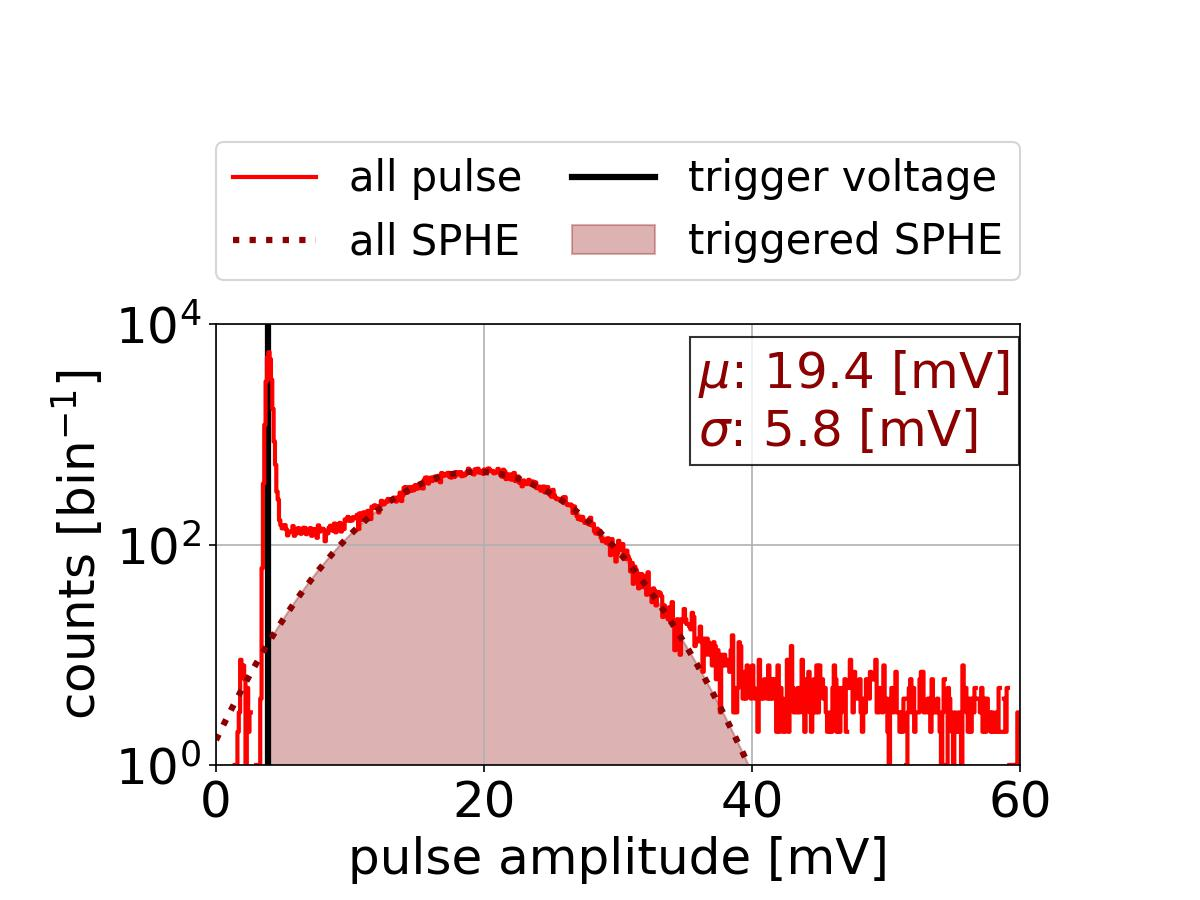
\includegraphics[width=\textwidth,clip,trim={0 0 0 0},angle=0,origin=c]{Figures/GasTest/DatasetQuality/topPMTTriggerEfficiency65831.jpg}
		\caption{}
		\label{fig:PMTTriggerEff top}
	\end{subfigure}
	\begin{subfigure}[b]{\textwidth}
		\centering
		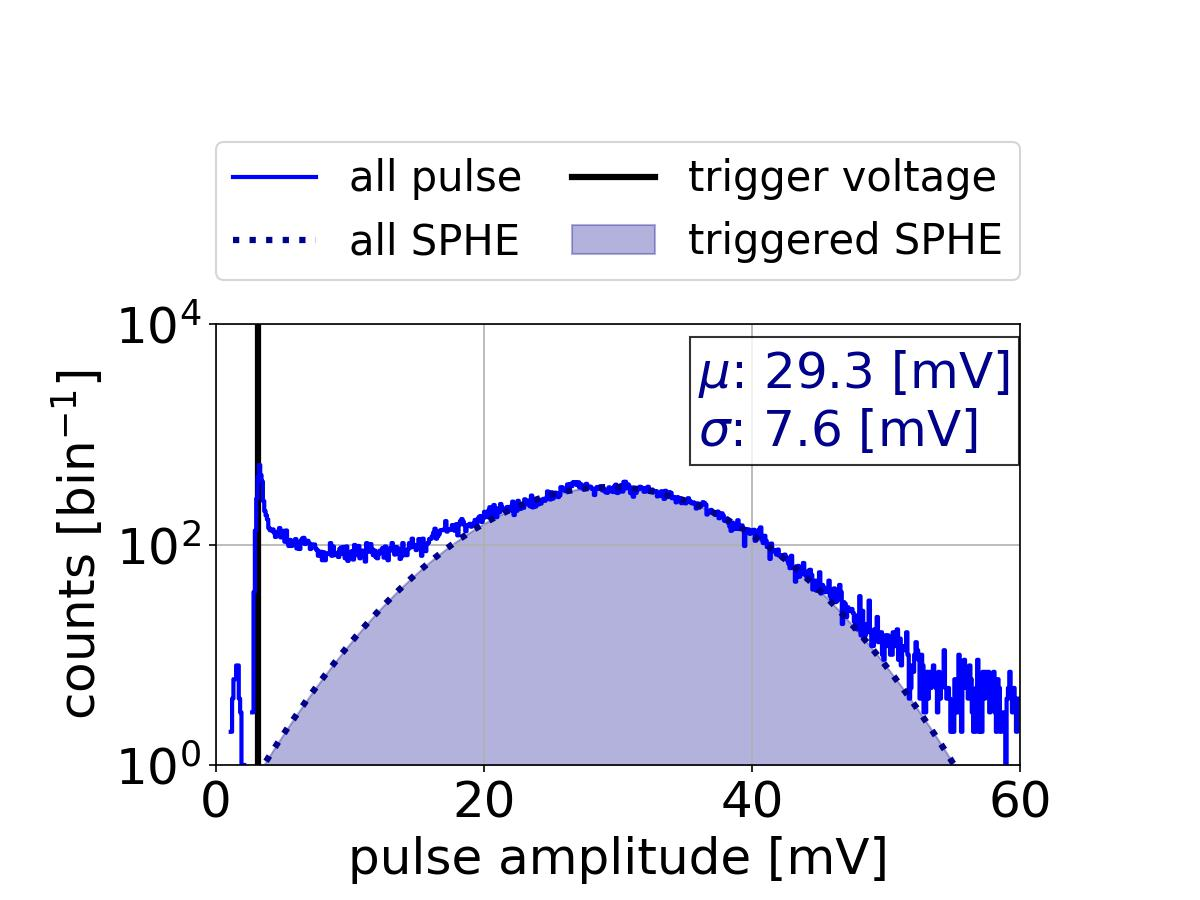
\includegraphics[width=\twofigurewidth,clip,trim={0 0 0 0}]{Figures/GasTest/DatasetQuality/botPMTTriggerEfficiency65831.jpg}
		\caption{}
		\label{fig:PMTTriggerEff bottom}
	\end{subfigure}
	\caption[PMT pulse amplitude distribution.]{PMT pulse amplitude distribution: (a) top PMT (b) bottom PMT. Data were taken at \ddtt{2018}{03}{12}{11}{41}.}
	\label{fig:PMTTriggerEff}
\end{figure}%code in '/Users/weiji/Google Drive/gastest/DatasetQuality/Baseline.py', wdir='/Users/weiji/Google Drive/gastest/DatasetQuality'

\paragraph{PMT \sphe\ pulse area}
 PMT \sphe\ pulse area is calibrated with fitting the pulse amplitude and integrated area to a two dimensional Gaussian distribution. Appropriate ranges of the pulse amplitude and pulse area are chosen to avoid the influence from noise and overlapping of multiple photo electrons this time. The chosen ranges are \SIrange{12}{28}{\mV}, \SIrange{0}{800}{\mV\ns} for the top PMT, and \SIrange{22}{38}{\mV}, \SIrange{0}{1000}{\mV\ns} for the bottom PMT. These chosen ranges contain the \sphe\ peaks of the particular PMTs ,which are identified as the brightest segments above the noise and are attributed to dark current. The used fitting function is, 
 \begin{align}
 z = 	A \exp \bigg( -\Big(\frac{1}{2 \sigma_x^2} \big( (x-\mu_{x})\cos \theta - (y-\mu_y)\sin \theta \big) ^2 + \frac{1}{2 \sigma_y^2} \big( (x-\mu_{x})\sin \theta + (y-\mu_y)\cos \theta \big) ^2  \Big) \bigg)
 \end{align} 
where x is the pulse area; 

y is the pulse amplitude; 

z is the total counts at each pulse area and amplitude, represented in the color scale; 

A is the amplitude of the fit; 

$\mu_{x}$ is the position of the center of the peak on x axis; 

$\sigma_{x}$ is the standard deviation on rotated x axis; 

$\mu_{y}$ is the position of the center of the peak on y axis; 

$\sigma_{y}$ is the standard deviation on rotated y axis; 

and $\theta$ is the rotated angle.  

The average values of the pulse area and pulse amplitude are $\mu_{x}$ and $\mu_{y}$. The standard deviation values of the pulse area and pulse amplitude are $\sigma_{x} \cos \theta - \sigma_{y} \sin \theta$ and $\sigma_{x} \sin \theta + \sigma_{y} \cos \theta$. Results of these fits are shown in Fig.~\ref{fig:PMTAmpArea}. Results of the PMT calibrations are summarized in Table~\ref{tab:PMTparameters}. Fitting values of different datasets show an agreement within \SI{1}{\percent} of the average PMT \sphe\ pulse area and pulse amplitude. 

The \sphe\ pulse amplitudes are approximately \SI{20}{\mV} for the top PMT and \SI{30}{\mV} for the bottom PMT. Thus, a simple estimation based on the dynamic range \SI{1260}{\mV} noted previously shows that the DAQ system allows approximately 60 \sphe s to be simultaneously recorded by the top PMT without distortion to the pulse shape, and 40 \sphe s for the bottom PMT. This dynamic range of simultaneous photon recording is large enough for recording \ees s without distortion to pulse shape in most situations. 

Degradation of the PMTs is not noticed during the run, even though the possibility of the degradation of the PMTs is discussed in their manual (Ref.~\cite{HamamatsuPhotonics2006}). Therefore, since this effect is not observed during the tests, for consistency of studying, the same value is used through all the studies for the average \sphe\ pulse area of each PMT. 

There are two revisions of these values of SPHE pulse area. In revision 1 (Rev1), the values used are \SI{426}{\mV\ns} for the top PMT and \SI{638}{\mV\ns} for the bottom PMT. The results in Rev 1 are from analyzing pulse area on datasets taken with the detector filled with xenon gas, and \opvtvb\ higher than \SI{0}{\kV}. These datasets may contains more contamination pulses other than \sphe pulses, e.g. multiple photon electron pulses, and therefore biased the estimation. In revision 2 (Rev2), only data taken at vacuum condition with \opvtvb\ at \SI{0}{\kV} are used. The results in Rev 2 are \SI{413}{\mV\ns} for the top PMT and \SI{610}{\mV\ns} for the bottom PMT. Rev2 gives a better estimation of the \sphe\ pulse area. The \sphe\ pulse area is referred to PHE as the unit of the PMT pulse area.

\begin{figure}[!p]
	\centering
	\begin{subfigure}[b]{\twofigurewidth}
		\centering
		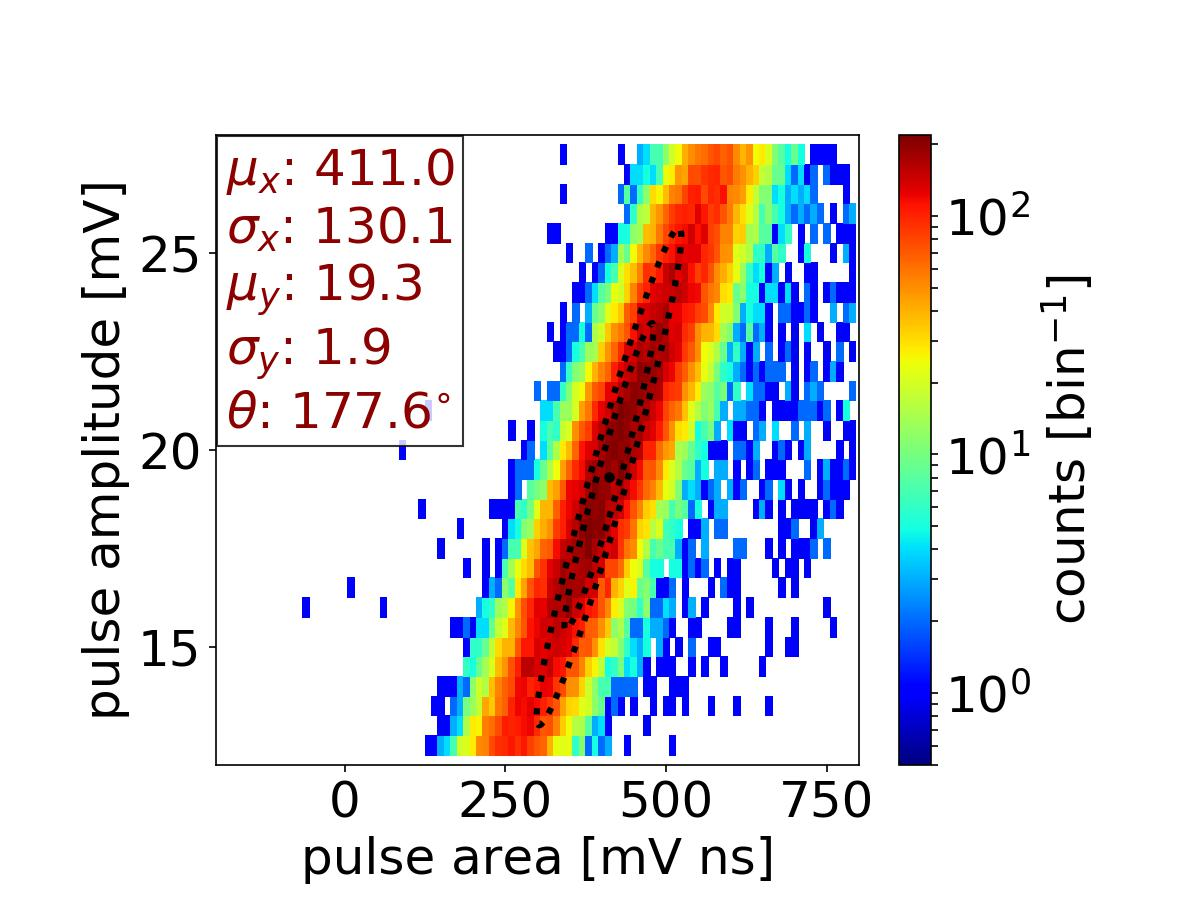
\includegraphics[width=\textwidth,clip,trim={0 0 0 0},angle=0,origin=c]{Figures/GasTest/DatasetQuality/topPMTArea65831.jpg}
		\caption{}
		\label{fig:PMTAmpArea top}
	\end{subfigure}
	\begin{subfigure}[b]{\twofigurewidth}
		\centering
		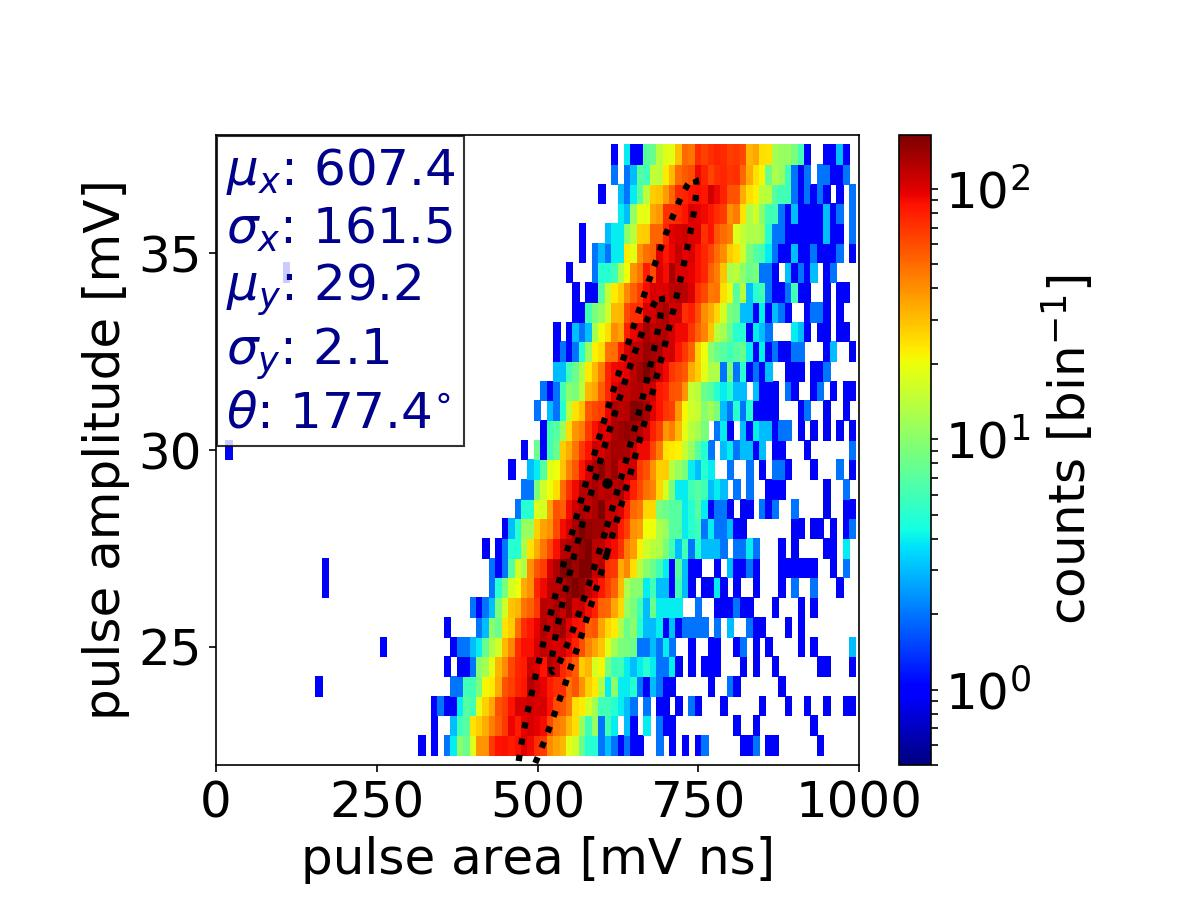
\includegraphics[width=\textwidth,clip,trim={0 0 0 0}]{Figures/GasTest/DatasetQuality/botPMTArea65831.jpg}
		\caption{}
		\label{fig:PMTAmpArea bottom}
	\end{subfigure}
	\caption[PMT \sphe\ pulse amplitude vs. pulse area distribution.]{PMT \sphe\ pulse amplitude vs. pulse area distribution: (a) top PMT (b) bottom PMT. The black dot, and the dashed line are the average, \SI{68}{\percent}, and \SI{95}{\percent} contours of the Gaussian fits. Data were taken at \ddtt{2018}{03}{12}{11}{41}.}
	\label{fig:PMTAmpArea}
\end{figure}

%\todo{think about whether to delete the first vacuum data in the table.}
	\begin{table}[!h]
	\centering
		\begin{tabular}[!h]{ | m{10em} ||m{5em} |m{5em} | m{5em} | m{5em}| m{5em}|} 
		\hline
		time & PMT name & trigger \mbox{voltage}  & trigger \mbox{efficiency} & pulse \mbox{amplitude}  & pulse \mbox{area} \\
   & & [\si{\mV}] & & [\si{\mV}] & [\si{\mV\ns}]
		\\\hline\hline

%        \ddtt{2017}{08}{26}{11}{53}* & top & 3.679 & 0.997 & \num{18.4 \pm 4.1} & \num{395 \pm 118}   \\\cline{2-6}& bottom & 2.629& 1.000 & \num{28.6 \pm 6.0} & \num{599 \pm 155}\\\hline %proc33001

        \ddtt{2018}{02}{03}{13}{21} & top & 3.762 & 0.997 & \num{19.4 \pm 3.3} & \num{413 \pm 132}   \\\cline{2-6}& bottom & 3.103& 1.000 & \num{27.9 \pm 4.6} & \num{607 \pm 161}\\\hline %proc10201
		
		\ddtt{2018}{03}{12}{11}{41} & top & 3.853 & 0.996 & \num{19.3 \pm 3.5} & \num{411 \pm 130}   \\\cline{2-6}& bottom & 3.130& 1.000 & \num{29.2 \pm 5.1} & \num{607 \pm 161}\\\hline %proc65831
		


%		\ddtt{2018}{03}{16}{17}{49} & top & 3.788 & 0.996 & \num{19.4 \pm 3.4} & \num{413 \pm 128}   \\\cline{2-6}& bottom & 3.269& 1.000 & \num{29.4 \pm 5.3} & \num{614 \pm 164}\\\hline %proc65901
				
		\ddtt{2018}{05}{15}{12}{03} & top & 3.713 & 0.997 & \num{19.4 \pm 3.5} & \num{413 \pm 131}   \\\cline{2-6}& bottom & 3.091& 1.000 & \num{29.5 \pm 5.4} & \num{615 \pm 167}\\\hline %proc13001
%		\ddtt{2017}{12}{08}{14}{42} & top & 3.914 & 0.996 & \num{20.1 \pm 3.8} & \num{426 \pm 136}   \\\cline{2-6}& bottom & 3.245& 0.999 & \num{30.7 \pm 5.9} & \num{638 \pm 177}\\\hline
%		\ddtt{2018}{06}{06}{02}{35} & top & 3.932 & 0.996 & \num{19.9 \pm 3.7} & \num{423 \pm 133}   \\\cline{2-6}& bottom & 3.403& 1.000 & \num{30.5 \pm 5.8} & \num{633 \pm 173}\\\hline

		\hline
adopted value (Rev1)& top & - & 1  & - & \num{426}   \\\cline{2-6}& bottom & - & 1  & - & \num{638}\\\hline %proc65831
adopted value (Rev2)& top & - & 1  & - & \num{413}   \\\cline{2-6}& bottom & - & 1  & - & \num{610}\\\hline %proc65831

	\end{tabular}
	
	\caption[PMT calibration.]{PMT \sphe\ calibration. 
		%*: DAQ setting for trigger voltage, post-delay, and number of sample trimmed at the end are different. The number of samples kept after post-threshold are the same. 
	}
 \label{tab:PMTparameters}
	\end{table}

\section{Light Collection}
\label{sec:gtest light collection}
\gtest\ evaluates event-based primary scintillation light and EL light. Light collection efficiency is important to understand the overall sensitivity of the detector.  Light collection is evaluated by the ratio of the number of photoelectrons observed for an event to the number of photons produced in this event;
\begin{align}
\text{light collection efficiency} = \frac{\text{\#\  photoelectrons observed for an event}}{\text{\#\  photons produced in an event}}.
\end{align}

Light collection efficiency includes geometric collection efficiency and PMT overall quantum efficiency. Geometric collection efficiency describes the efficiency of photon propagation to reach PMT photocathode surfaces, which includes photon propagation in the gas medium, photon reflection by the detector material surfaces, and photon propagation in PMT window materials. PMT overall quantum efficiency describes the efficiency of how many photons are absorbed by the photocathode surfaces and turn into measurable current or voltage signals.

\paragraph{Geometric collection efficiency} Geometric collection efficiency is studied by photon propagation simulation software Light Guide, as described in Ref.~\cite{Shutt2018}. In the simulation software, a simplified \gtest\ detector boundary with cylindrical symmetry is drawn to represent the real detector material surfaces.  This simplified geometry includes the photocathode surfaces of the PMTs, inner surfaces of the PTFE cones, and surfaces of the grid rings. In addition, each grid is represented by two planes of parallel wires with the same diameter and the same distance between two parallel wires as in the real detector. The two planes are parallel to each other and close in distance to represent two distinct sets of wires interlacing each other.  %This software is capable of simulating photon propagation in the transparent or translucent medium using the physics quantity scattering and absorption of the medium. 
Photon absorption and reflection, which takes into account  the probability of specular reflection and Lambretian diffusion reflection, are simulated at material surfaces. The empty space inside the simplified detector geometry is filled with a transparent or translucent medium. The simulation of photon propagation through the medium includes scattering and absorption effects.

The uncertainty of the reflectivity of detector surface materials has a major influence on the total light collection. Among these materials, PTFE reflectivity has the largest uncertainty reported, the value of which for xenon scintillation photons at room temperature are in the range of \numrange{0.4}{0.75}. This difference in reflectivity may be a result of different fabrication %synthetic 
processes or different material density, as discussed in Ref.~\cite{Silva2009}.

The geometric collection efficiency is evaluated as a function of (r, z) in the detector. To understand geometric collection efficiency at one specific location, \numrange{e5}{e7} simulations of single photons are generated from this specific location. % in a cylindrical coordinate system, (r, z). 
Each simulated photon is stepped either to transport through the detector medium or to interact with the detector surface materials. Each simulation ends when the simulated photon is absorbed by either the detector medium or detector surface materials. The counts of photons reaching PMT photocathode surfaces are used to estimate geometric collection efficiency,  
\begin{align}
	\text{Geometric collection efficiency} = \frac{\text{\#\  photons reaching PMT photocathode surfaces}}{\text{\#\  photons simulated}}
\end{align}

\paragraph{PMT overall quantum efficiency} 
The overall quantum efficiency of a PMT includes (1) the PMT photocathode quantum efficiency (QE), (2) the PMT electron collection efficiency, and (3) the PMT electron gain.

The PMT photocathode QE is the probability per incident photon to produce a photoelectron. For 175 nm xenon scintillation light, there is a \SI{\sim 20}{\percent} probability for 2 photoelectrons to be produced rather one, so called the double photoelectron effect. We use the term photons detected (PHD) to refer to the number of photons that produced at least one photoelectron. The term PHE refers to the number of photoelectrons produced at the photocathode. The photocathode quantum efficiency for the top and bottom PMTs, as quoted by Hamamatsu, are \SI{36.3}{\percent} and \SI{36.0}{\percent}, respectively, for \SI{175}{\nm} light, see Table~\ref{tab:PMTparameterHamamatsu}. The Hamamatsu QE does not account for the double photoelectron effect; that is, it is the average number of photoelectrons produced per incident photon, different from the average number of photons that produce a measurable signal per incident photon.

%PMT response includes (1) PMT quantum efficiency (Q.E.)., (2) PMT electron collection efficiency ,and (3) PMT electron gain. 

%PMT Q.E. is the ratio of output photoelectrons to incident photons. It is the efficiency of photoelectric effect including the probability of photoelectric effect creating multiple photoelectrons from a single photon (double photoelectrons effect).  
%We use counts of photoelectrons detected (PHD) to describe the counts of photons detected without the influence of double photoelectrons effect, and counts PHE to describe the counts of photons detected with the influence of double photoelectrons effect. 
%Statistical average one PHD is approximately \num{1.2} PHE. PHE is the unit that is used in this analysis. 
%In this simulation, values of PMT Q.E. at \SI{175}{\nm} are used. They are \SI{36.3}{\percent} for the top PMT and \SI{36.0}{\percent} for the bottom PMT, see Table~\ref{tab:PMTparameterHamamatsu}. 

PMT electron collection efficiency is the probability that these output photoelectrons land on the effective area of the first dynode; the mechanism of how the PMT works is described in Section~\ref{sec:gtest dectector}. %This landing makes the electrons go to the next dynode, thus being multiplied by the chains of dynodes. 
PMT electron collection efficiency depends on the mechanical design of a PMT and the voltage difference between the PMT photocathode and the PMT first dynode. The exact value of electron collection efficiency of the PMTs used in \gtest\ at their operating voltage are not measured. We estimate PMT electron collection efficiency to be \SI{90}{\percent} based on measurement of other PMTs of the same model at a higher PMT operating voltage, as described in Ref.~\cite{Lung2012}.
	%,Akerib2013b

PMT electron gain describes the multiplication process of the output photoelectrons in dynode stages. The current that results from this multiplication process is translated to voltage using a \SI{50}{\ohm} load resistor. The multiplication process amplifies the useful signal and eases the signal noise selection. The voltage then is digitized by the DAQ, as described in Section~\ref{sec:gtest daq}. The digitized voltage is the measured PMT signals. Observed signals are translated to units of PHE by dividing out the average \sphe\ area for each PMT. %The average value of the PMT signal pulse area of one photoelectron is the average \sphe\ pulse area in PMT calibration. 
The coefficient of variation (CV, the ratio of the standard deviation to the average value) of PHE is \SI{\sim 30}{\percent}, as described in Section~\ref{sec:pmt cal}. 

\paragraph{}
Therefore, to understand the spatial dependence of light collection efficiency in the ELD, we start with \num{500000} simulations of single photons every \SI{5}{mm} in r and z dimension in the ELD, and record the geometric collection efficiency of each location. This number is then multiplied by PMT overall QE to obtain the total light collection efficiency. There are two light collection efficiency estimation of two different grid wire configurations that we used for grid emission tests, labeled grid configuration~1 (grid config.~1) and grid configuration~2 (grid config.~2). Run 4 to Run 9 use grid configuration~1, and Run 10 to Run 17 use grid configuration~2. These two configurations are identical everywhere else in the ELD except for the wire diameter and the distance between two parallel wires of the top grid. Table~\ref{tab:LC sim parameter geo} and Table~\ref{tab:LC sim parameter material} summarize the parameters in the simulation.

	\begin{table}[!h]
		\centering
		\begin{tabular}[!h]{ | m{8em} m{20.5em} || m{4.5em} | m{4.5em}|} 
			\hline
				&parameter & grid config.~1 & grid config.~2 \\
				& & Run 4-9 & Run 10-17  \\\hline\hline			
		    top grid & distance between two parallel wires [\si{\mm}] & 2.5	 & 5\\
		    			 & wire diameter [\si{\um}] &  100  & 150 \\\hline
		    bottom grid & distance between two parallel wires [\si{\mm}] & 2.5	 & 2.5 \\
		    			 & wire diameter [\si{\um}] &  75  & 75  \\\hline
		    top/bottom cone %& height total [\si{\mm}] & 110 & 110 \\
		                & cylinder 1 height [\si{\mm}] & 1.17 & 1.17 \\
		    (PTFE reflector) 		& cylinder 1 radius (frustum larger radius) [\si{\mm}] & 65 & 65 \\
		    			    & frustum height [\si{\mm}] & 98.8 & 98.8 \\
		    			& cylinder 2 radius (frustum smaller radius) [\si{\mm}] & 32 & 32 \\
		    			& cylinder 2 height [\si{\mm}] & 10 & 10 \\\hline
		    top/bottom PMT & photocathode radius [\si{\mm}] & 32 & 32 \\
		    \hline		    
		\end{tabular}
		\caption[Light collection simulation geometry parameters.]{Light collection simulation geometry parameters}
		\label{tab:LC sim parameter geo}
	\end{table}


	\begin{table}[!h]
		\centering
		\begin{tabular}[!h]{ | m{12em} m{16em} || m{10em}|} 
			\hline
			&parameter &    value \\\hline\hline
			Xe (gas)   
			& refraction index & 1.544 \\
			& Rayleigh scatter length [m] & 500 \\
							& absorption length [m] &	500  \\
							\hline
			Quartz (synthetic quartz)   
				& refraction index & 1.000702 \\
							\hline
			PTFE 	   
			& reflectivity & 0.4 (0-1.0) (Ref.~\cite{Feuerbacher1972}) \\
						  &	 specular reflection ratio & 0\\
						  & Lambretian diffusion reflection ratio & 1\\
						  \hline
			SS (SS304)   & reflectivity & 0.18 (Ref.~\cite{Feuerbacher1972}) \\
						& specular reflection ratio & 1\\
						& Lambretian diffusion reflection ratio & 0\\
			\hline    
		\end{tabular}
		\caption[Light collection simulation material parameters.]{Light collection simulation material parameters}
		\label{tab:LC sim parameter material}
	\end{table}

As expected, the geometric collection efficiency varies at different locations in the ELD, which causes the light collection efficiency to vary, accordingly. %(Wei used to have)Geometric collection efficiency varies at different spacial locations in the detector and cause light collection efficiency also varies. 
The light distribution between the top and bottom PMT also varies across the ELD. This light distribution helps discriminate the location where events happened. We use top-bottom asymmetry (TBA) to describe this light distribution, which is defined as: 

\begin{align}
	\text{TBA} = \frac{\text{Top PMT light collection}-\text{Bottom PMT light collection}}{\text{Top PMT light collection}+\text{Bottom PMT light collection}}.
\end{align}

%Fig.~\ref{fig: light collection cross section 040} shows results of the simulations. 
Results in Fig.~\ref{fig: light collection cross section 040} show the light collection efficiency and the TBA in the ELD. Locations that are in the top cone region usually have a positive TBA, and locations that are in the bottom cone usually have a negative TBA. TBA is close to zero in the EL region. 

Among all different classes of events, our primary pulse of interest is \eee s, which happen in the EL region. We estimate the light collection in this region with the same method mentioned before and finer binning. We start with \num{500000} simulations of single photons every \SI{2}{\mm} in r dimension in the middle of the EL region.  Results of the simulations are shown in Fig.~\ref{fig: light collection r 040}. Light collection efficiency in the EL region falls away at r \SI{> 65}{\mm}, which is the inner radius of the PTFE reflector cones. %The TBA also changes at r > \SI{65}{\mm}. 
The average top and bottom PMT light collection efficiencies in the EL region are \num{\sim 0.0085}. The average TBA in the EL region is \num{\sim 0}. The average total PMT light collection efficiency in the EL region is \num{\sim 0.017}. For most \eee s in which photon production is larger than \num{300}, an average number of \num{\sim 5} photoelectrons would be observed. Therefore, this light collection efficiency is sufficient to allow us to detect \eee s.

The uncertainty of PTFE reflectivity has a large influence on the total light collection, %.  The influence on the total PMT light collection 
which is shown in Fig.~\ref{fig: light collection vs. PTFE ref}. Higher PTFE reflectivity results in a higher total light collection efficiency. The actual value of reflectivity of the PTFE reflector cones has not been measured directly. We estimate the actual PTFE reflectivity of xenon scintillation photons to be \num{0.4}, according to the material density . 

\begin{figure}[!p]
	\centering
	\begin{subfigure}[b]{\halfwidth}
		\centering
		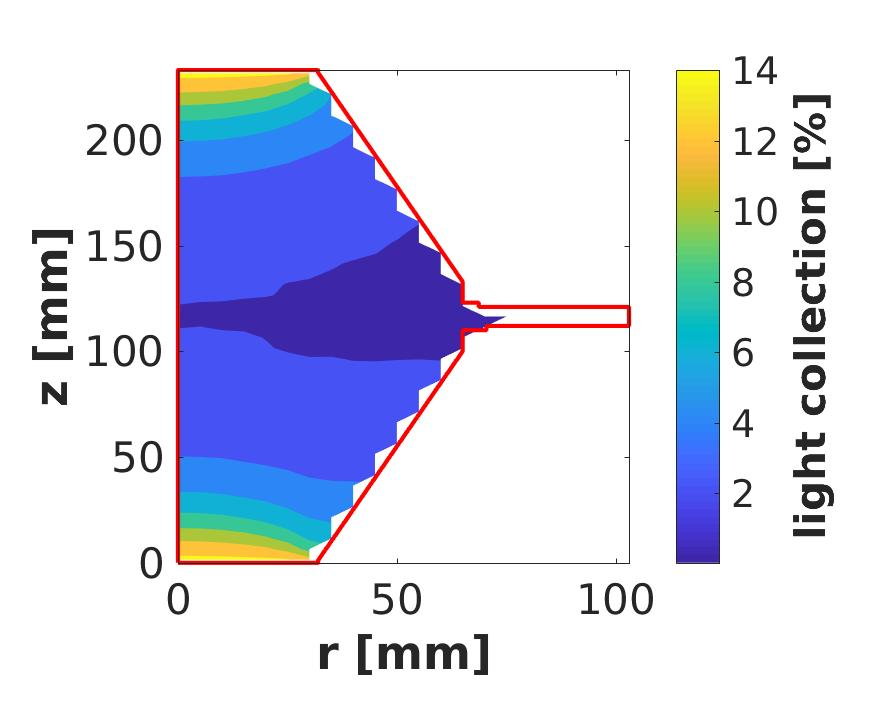
\includegraphics[width=\textwidth,clip,trim={0 0 0 0}]{Figures/GasTest/LGresult/PDEvsCrossSectionTotPTFE040.jpg}
		\caption{}
		\label{fig:}
	\end{subfigure}
	\begin{subfigure}[b]{\halfwidth}
		\centering
		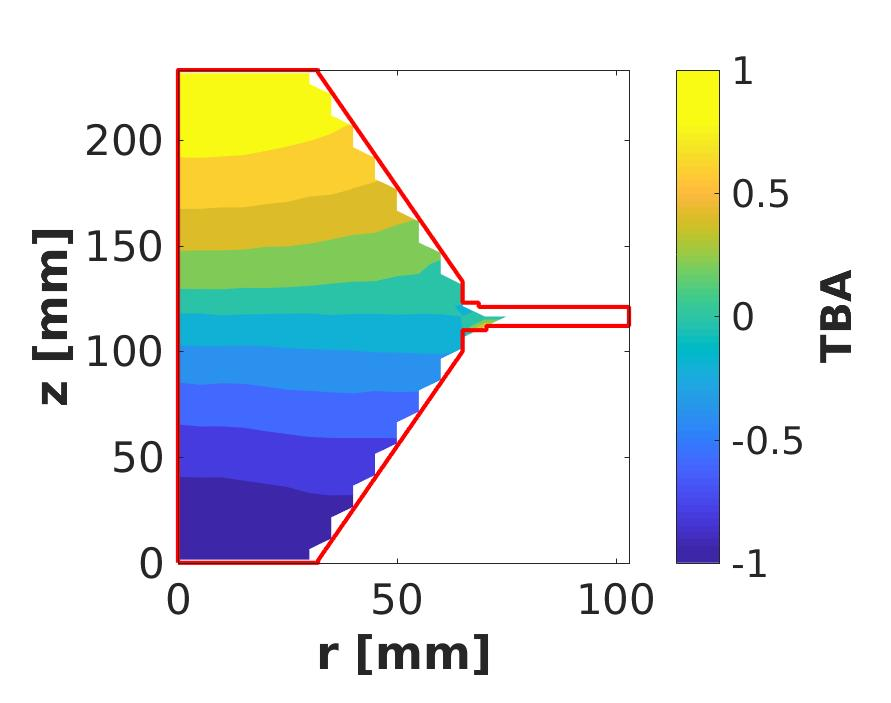
\includegraphics[width=\textwidth,clip,trim={0 0 0 0}]{Figures/GasTest/LGresult/PDEvsCrossSectionTBAPTFE040.jpg}
		\caption{}
		\label{fig:}
	\end{subfigure}
	\begin{subfigure}[b]{\halfwidth}
		\centering
		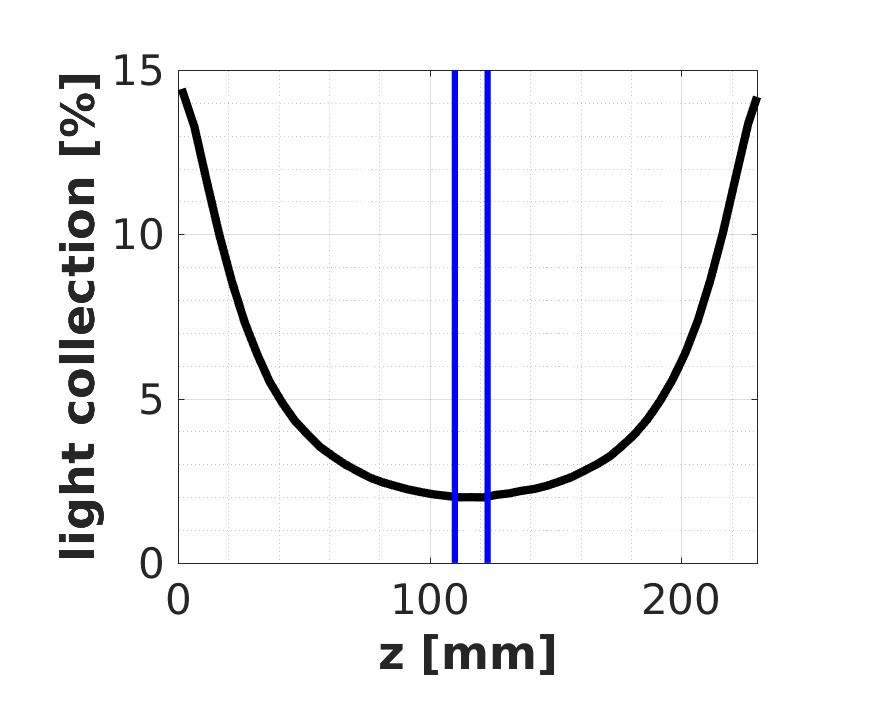
\includegraphics[width=\textwidth,clip,trim={0 0 0 0}]{Figures/GasTest/LGresult/PDEvsCrossSectionzTotPTFE040.jpg}
		\caption{}
		\label{fig:}
	\end{subfigure}
	\begin{subfigure}[b]{\halfwidth}
	\centering
	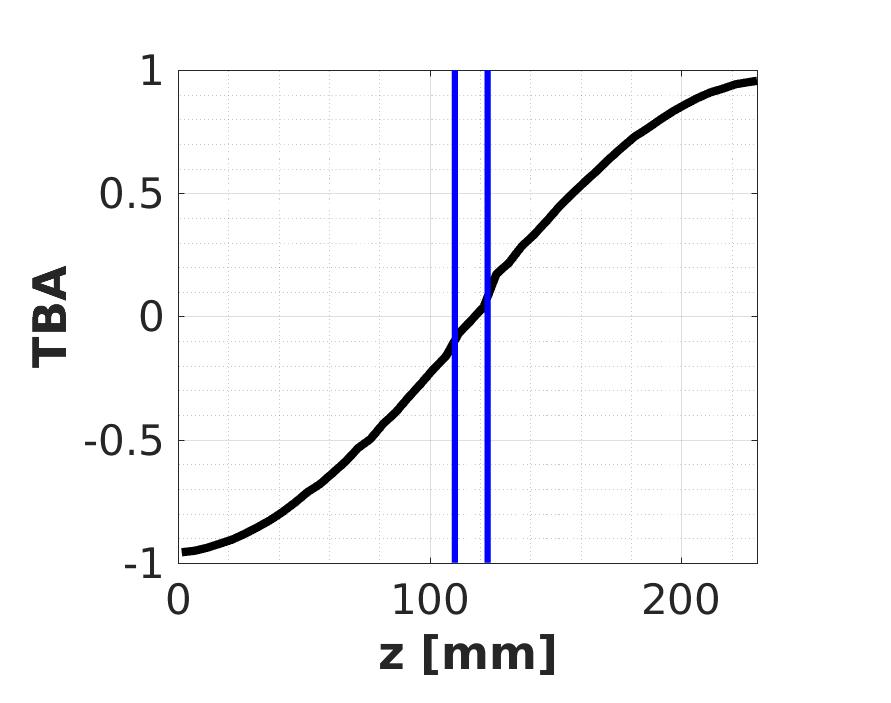
\includegraphics[width=\textwidth,clip,trim={0 0 0 0}]{Figures/GasTest/LGresult/PDEvsCrossSectionzTBAPTFE040.jpg}
	\caption{}
	\label{fig:}
\end{subfigure}
	%	\caption[]{(a)  (b) (c)}
	\caption[Light collection efficiency of (r, z) cross section in the ELD from simulation.]{Light collection efficiency of (r, z) cross section in the ELD from simulation. (a) Total light collection efficiency. (b) Top-bottom asymmetry (TBA). (c) Total light collection efficiency at r=0. (d) TBA at r=0. The red solid curve is the edge of the active volume of the ELD. The blue solid curve is the edges of the EL region. This result uses configuration 1, PTFE reflectivity \num{0.40}. z=0 is at the bottom PMT photocathode surface.}
	\label{fig: light collection cross section 040} % code is in `"/media/wei/ACA8-1ECD3/CleanAmendedLightGuide/CleanAmendedLightGuide/LightGuide/UserRoutines/Plotting/Phase1/PlotRealLight20180110GasTestGeo.m
\end{figure}

\begin{figure}[!p]
	\centering
	\begin{subfigure}[b]{\halfwidth}
		\centering
		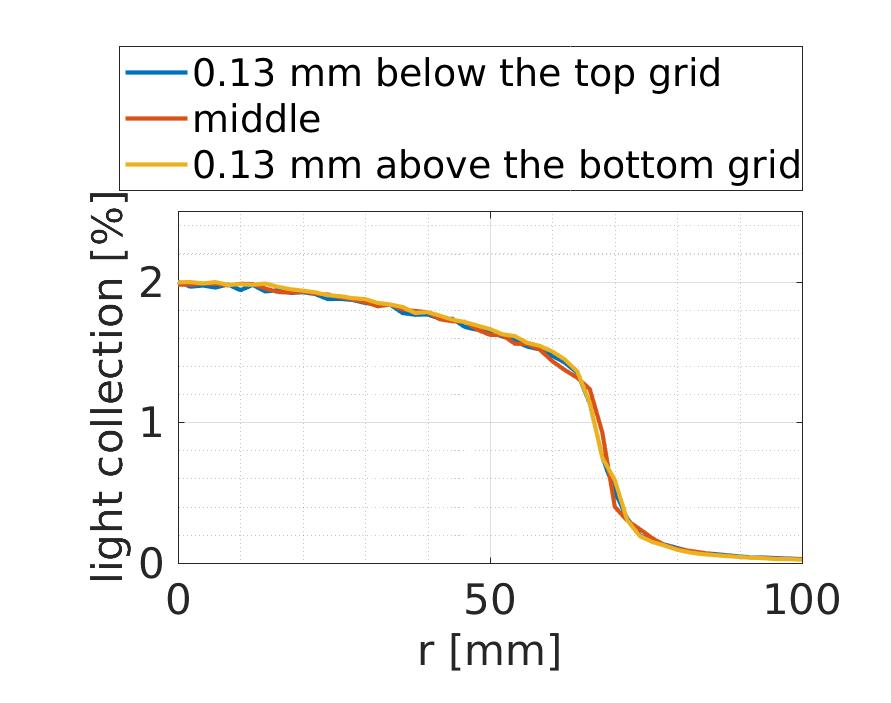
\includegraphics[width=\textwidth,clip,trim={0 30 0 195}]{Figures/GasTest/LGresult/PDEvsRadiusPTFE040MiddleTopBottomconfig1.jpg}
		\caption{}
		\label{fig:}
	\end{subfigure}
	\begin{subfigure}[b]{\halfwidth}
		\centering
		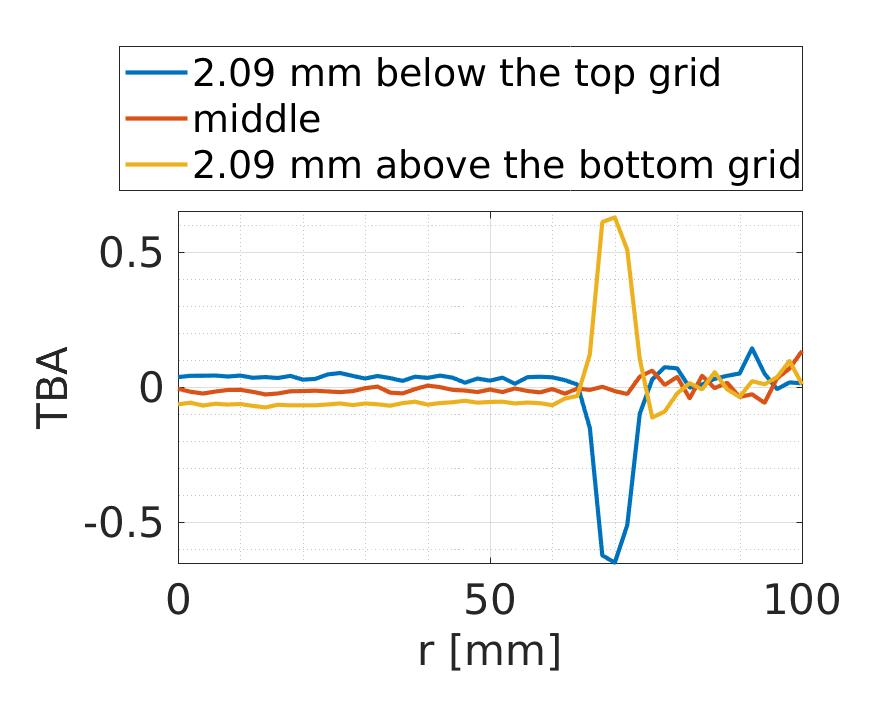
\includegraphics[width=\textwidth,clip,trim={0 30 0 200}]{Figures/GasTest/LGresult/PDEvsRadiusPTFE040MiddleTopBottomTBAFullconfig1.jpg}%,trim={0 0 0 180}]{Figures/GasTest/LGresult/PDEvsRadiusPTFE040MiddleTopBottomTBAconfig1.jpg}
		\caption{}
		\label{fig:}
	\end{subfigure}

	\begin{subfigure}[b]{\halfwidth}
	\centering
	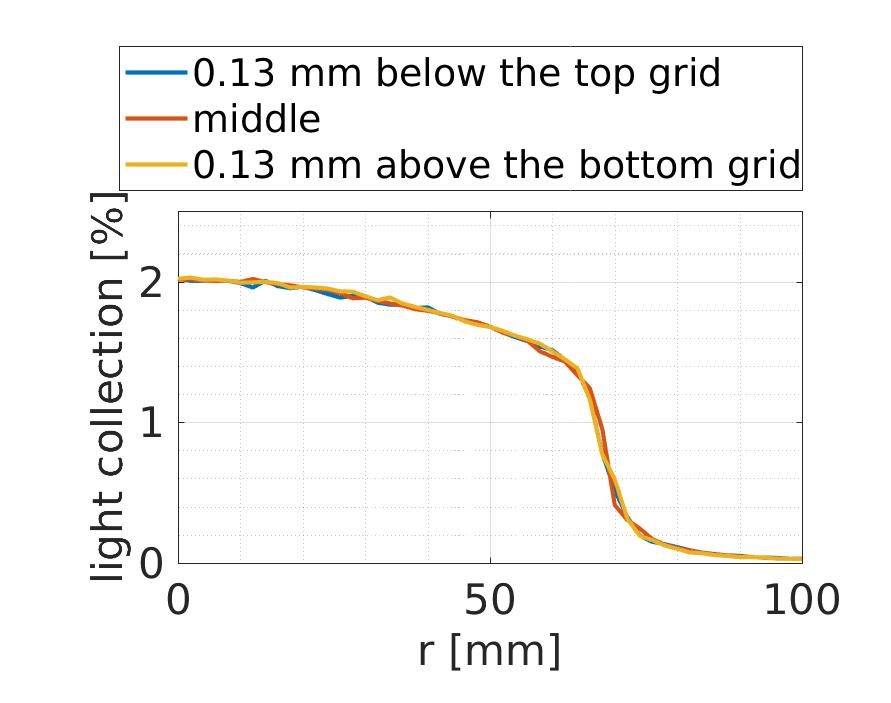
\includegraphics[width=\textwidth,clip,trim={0 30 0 195}]{Figures/GasTest/LGresult/PDEvsRadiusPTFE040MiddleTopBottomconfig2.jpg}
	\caption{}
	\label{fig:}
\end{subfigure}
\begin{subfigure}[b]{\halfwidth}
	\centering
	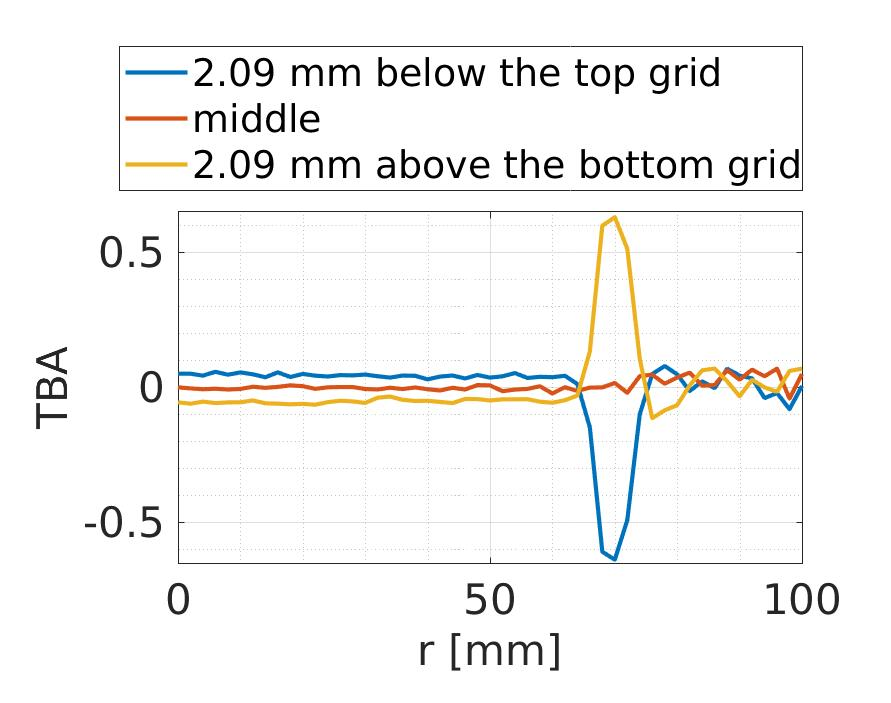
\includegraphics[width=\textwidth,clip,trim={0 30 0 200}]{Figures/GasTest/LGresult/PDEvsRadiusPTFE040MiddleTopBottomTBAFullconfig2.jpg}%,trim={0 0 0 180}]{Figures/GasTest/LGresult/PDEvsRadiusPTFE040MiddleTopBottomTBAconfig2.jpg}
	\caption{}
	\label{fig:}
\end{subfigure}

	%	\caption[]{(a)  (b) (c)}
	\caption[Light collection efficiency and TBA in the EL region in different grid configurations from simulation.]{Light collection efficiency and TBA in the EL region in different grid configurations from simulation. (a) Total light collection efficiency in grid configuration~1. (b) TBA in grid configuration~1. (c) Total light collection efficiency in grid configuration~2. (d) TBA in grid configuration~2. The blue curve shows the value (light collection efficiency or TBA) as a function of r for fixed \SI{2.09}{\mm} below the top grid. The yellow curve shows the value as a function of r for fixed \SI{2.09}{\mm} above the bottom grid. The red curve shows the value as a function of r at the midpoint between the top and bottom grids. Light collection efficiency decreases and TBA has a sharp feature at r=\SI{65}{\mm}, which is the inner diameter of the PTFE reflector cones. This result uses PTFE reflectivity \num{0.40}.}
	\label{fig: light collection r 040} 
	%The blue curve shows the value (light collection efficiency or TBA) as a function of r for fixed 2.09 mm below the top grid. The yellow curve shows the value as a function of r….. The red curve shows the value as a function of r at the midpoint between the top and bottom grids. (Alden)
	% code in "/media/wei/ACA8-1ECD3/CleanAmendedLightGuide/CleanAmendedLightGuide/LightGuide/UserRoutines/Plotting/Phase1/CPlotRealLight20180110GasTestGeo.m
\end{figure}



% \begin{figure}[!ht]
%   \centering
%   \includegraphics[width=0.6\textwidth,clip,trim={0 0 0 170}]
%   {Figures/Ch10/PDEvsRadiusPTFE075.jpg}
%   \includegraphics[width=0.6\textwidth]
%   {Figures/Ch10/PDEvsRadiusPTFE075MiddleCircle.jpg}
%   \caption{Light collection efficiency(PDE) inside the detector region between anode grid and gate grid(simulated with PTFE reflectivity of $0.75$). Top: light collection efficiency vs. radius from the center of the grid ring at different location. Blue: 2 mm above the gate grid. Red: in the middle between the anode grid and the gate grid. Yellow: 2 mm below the anode grid. Bottom: light collection efficiency in the middle between the anode grid and the gate grid. Red solid curve is the region of the grid wires. }
%   \label{fig: light collection r 075}
% \end{figure}

\begin{figure}[!p]
	\centering
	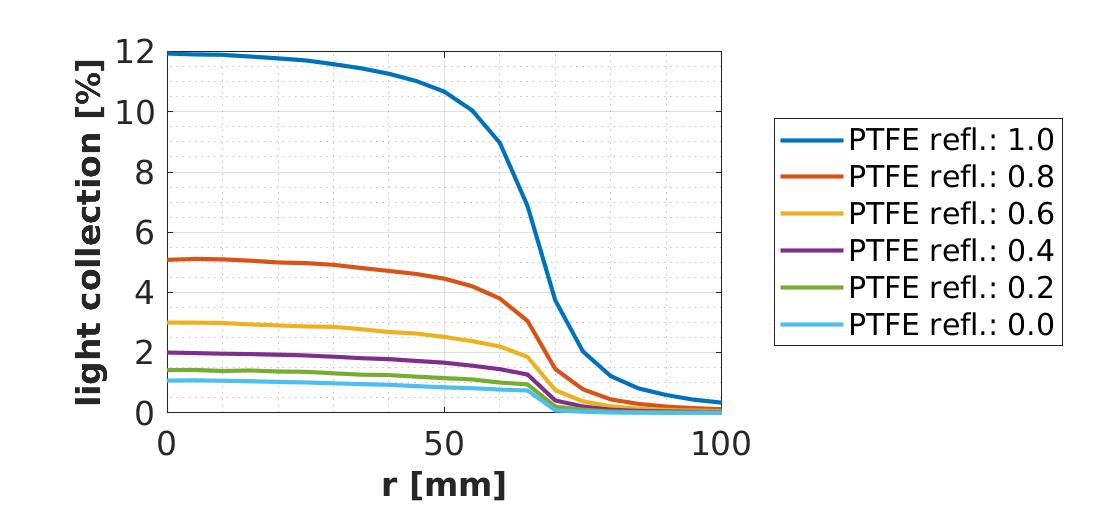
\includegraphics[width=.7\textwidth]
	{Figures/GasTest/LGresult/PTFESWeep.jpg}
	\caption[Light collection efficiency in the EL region with different PTFE reflectivity from simulation.]{Light collection efficiency in the EL region with different PTFE reflectivity from simulation. Light collection efficiency decreases at r = \SI{65}{\mm}, which is the inner diameter of the PTFE reflector cones. This result uses grid configuration~1.  }
	\label{fig: light collection vs. PTFE ref} % code in ""/media/wei/ACA8-1ECD3/CleanAmendedLightGuide/CleanAmendedLightGuide/LightGuide/UserRoutines/Plotting/Phase1/PTFEsweep.m
\end{figure}

%\begin{figure}[!ht]
%	\centering
%	\includegraphics[width=0.95\textwidth]
%	{Figures/Ch10/PhotonSim_TotalTime10000_T1090_MeanStd.jpg}
%	\includegraphics[width=0.95\textwidth]
%	{Figures/Ch10/PhotonSim_TotalTime10000_T1090_selectionEff.jpg}
%	\caption{Top: Mean and standard error of the distribution of the ratio between the time difference between 10\% integrated area and 90\% integrated area ($t1090$) and the total drift time($t\_total$). Bottom: the probability of $t1090/t\_total$ within the selected range.}
%	\label{fig: t1090 vs. photon num }
%\end{figure}
%
%\begin{figure}[!ht]
%	\centering
%	\includegraphics[width=0.95\textwidth]
%	{Figures/Ch10/SE_profile.jpg}
%	\caption{The number of photons collected per electron. Blue curve is simulated assuming 1000 photons are created per electron, PTFE reflectivity=$0.4$, electron collection efficiency=$0.9$. Green curve is the closest fit with binomial profile.}
%	\label{fig: single electron size from sim}
%\end{figure}

%\begin{figure}[!ht]
%	\centering
%	\includegraphics[width=0.6\textwidth,clip,trim={0 0 0 170}]
%	{Figures/Ch10/OnePMTPDEvsRadiusPTFE040.jpg}
%	\includegraphics[width=0.6\textwidth,clip,trim={0 0 0 170}]
%	{Figures/Ch10/OnePMTPDEvsRadiusPTFE075.jpg}
%	\caption{One PMT setup light collection efficiency(PDE) inside the detector region between anode grid and gate grid. Blue: 2 mm above the gate grid. Red: in the middle between the anode grid and the gate grid. Yellow: 2 mm below the anode grid. Top: PTFE reflectivity $0.40$. Bottom: PTFE reflectivity $0.75$. }
%	\label{fig: light collection r 040 one PMT}
%\end{figure}










\section{Light production}
\label{sec:gtest light procduction}
The ELD measures primary scintillation photons and electroluminescence photons in gas. First, I will introduce these two light production processes. Next, I will discuss the light production in noble gas, e.g. xenon, which is the medium that the ELD normally operates in. 

\paragraph{Primary scintillation} Primary scintillation is the process in which photons are created directly by energy deposition of external particle events. These photons have two sources: direct excitation, and excitation from recombination after ionization. An external particle travels through the medium in the ELD, transferring its energy to atoms in the medium, e.g. xenon, through exciting and ionizing these atoms. The excited atoms will return to their ground states by emitting photons of series energies corresponding to the energy level of the atoms, which is called relaxation of the excited atom. These photons from direct excitation from external particles are the first source of primary scintillation photons. The ionized atoms are not able to produce photons by themselves. However, they can recombine with the electrons around them and form excited atoms, which deexcite in a similar process as direct excited atoms, and emit photons simultaneously. These photons are the second source of primary scintillation photons. The quantity of second source of primary scintillation photons is dependent on the recombination process, which depends on properties of the atoms, and is influenced by the detector environment, especially the electric field (or reduced electric field) on the recombination site. A strong electric field forces electrons to quickly drift away from the ionization site and reduce the probability of recombination, thus reducing the quantity of primary scintillation light production. 
%These two primary scintillation processes happen fast in most medium.  

\paragraph{Electroluminescence} Electroluminescence (EL) is a phenomenon in which an electron drifts through a strong electric field in a medium, collides with atoms in the medium, excites them which will afterwards emit scintillation light. Since EL process is related to electrons in the medium, we measure EL photons to study the electron production in the detector. The mechanism of EL is similar to primary scintillation; the electron gains energy from drifting through the strong electric field and simultaneously loses energy though exciting and ionizing medium atoms. Moreover, the ionization process are usually associated with electron multiplication (gas gain), which creates more electrons in the strong electric field region, and produces more EL scintillation light. The quantity of EL scintillation photons and the probability of electron multiplication, are related to the strength of reduced electric field of the medium. With proper strength of reduced electric field, EL can produce more photons than primary scintillation. Because of its association with electrons and its production quantity, EL photons are the most important signals measured in the ELD.  

The primary scintillation photons are called \sone , and the EL scintillation photons are called \stwo , because the primary scintillation photons are produced earlier than the other photons created by electroluminescence process of uncombined electrons.  The same concepts of primary scintillation, as well as \sone\ and \stwo ,  are also used in liquid noble detectors, as described in Chapter.~\ref{chap:lz}. 

\paragraph{Noble gas scintillation}
For most noble gas atoms (\ce{A}), e.g. neon, argon, krypton, and xenon, the scintillation process usually forms an intermediate excited excimer state (\ce{A_2^*}). The emitted photons from the intermediate excimer state are almost monoenergetic, e.g. \SI{7.1}{\electronvolt} (\SI{\sim 175}{\nm}) in xenon, which  the medium is transparent to. Because of the existence of the intermediated excited excimer states, it creates appreciable quantity of monoenergetic photons from the deexcitation of these states. These features allow us to efficiently collect these monoenergetic photons with specialized devices, e.g. PMTs, and use these photons to study reactions between external particles and medium atoms.

The chemical processes of scintillation are:  
\begin{align}
\text{scintillation process: } & \ce{A + A^*  -> A_2^*}  \label{eqn:xenon sci 1}\\
& \ce{A_2^* ->A + A + \gamma }. \label{eqn:xenon sci 2}
\end{align}
where A is the noble gas atom; \ce{A^*} is the noble gas excited state; \ce{A_2^*} is the excimer state; $\gamma$ is the monoenergetic photons from deexcitation of the excimers; and the low energy photons produced during the process are not shown.

The chemical processes of recombination are:
\begin{align}
\text{recombination process: } & \ce{A + A^{+}  -> A_2^{+} } \\
& \ce{e^{-} + A_2^{+} ->A_2^* }\\%+ \gamma\prime} \\
\text{or: } & \ce{e^{-} + A^{+}  -> A^{*} } % + \gamma\prime}
\end{align}
%& \ce{Xe + Xe^*  -> Xe_2^*} \\
%& \ce{Xe_2^* ->Xe + Xe + \gamma},
where  \ce{A^+} is the noble gas ionized state; \ce{A_2^+} is the ionized dimer state; and the low energy photons produced during the process are not shown.% and$\gamma\prime$ is photons of other energy. 
The recombination process then leads to the same channels as the primary scintillation, with monoenergetic photons as the output signals. These photons, combined with photons from direct excitations, make primary scintillation light. 
%Both scintillation and recombination processes end up with deexcitation of excimers. The recombination process turn ions into excited atoms and excimers, which will deexcite similar as the scintillation process.  
The quantity of the monoenergetic photons is related to the reaction energy between external particles and medium atoms, and properties and physical environment of the medium (especially medium density and electric field). 

These two primary scintillation processes rapidly occur in xenon, the duration of which is dominated by the excimers decay time. The excimers can be separated into two types, the singlet state (\ce{^1\sigma_u^+}, \ce{0_u^+}) and triplet state (\ce{^3\sigma_u^+}, \ce{1_u^+}), with separate decay times. The singlet state and the triplet state are known to be created from a three-body deconstruction of noble gas atom excited state \ce{^2P_{1/2}} state and \ce{^2P_{3/2}} state, which has a different initial quantity from the event. Because these creation processes are three body reactions, the creation rate of the these two states have strong dependence on the gas density of atoms. The decay time of both of these two states have a dependence on the gas density, as described in  Ref.~\cite{Keto1974}. Some other materials also show that the decay time is very different between liquid noble gas and very dense noble gas. The decay time for the singlet state and the triplet state in liquid xenon are \SI[separate-uncertainty=false]{4.3 \pm 0.6}{\ns}  and \SI[separate-uncertainty=false]{22.0 \pm 2.0}{\ns}, as measured in Ref.~\cite{Hitachi1983}. For dense xenon with pressure in the range of \SIrange{2.7}{32}{\atm}, the decay time for singlet states varies from \SI[separate-uncertainty=false]{15 \pm 3}{\ns} to \SI[separate-uncertainty=false]{5.5 \pm 1.0}{\ns}. The decay time for triplet state is \SI[separate-uncertainty=false]{96 \pm 5}{\ns} in the same pressure range.

\todo{think about should I take about ionization/scintillation ratio here?}

EL photons, produced in gaseous xenon from the energy-loss of fast-moving electrons, are one of the most important signals that we measure. This EL process is driven by the electrons gaining energy in the electric field. This chemical process is,
\begin{align}
\text{EL process (direct excitation): } &\ce{e^- + A -> e^- + A^*} .
\end{align}
in which an electron directly excite a xenon atom. These excited-state atoms (\ce{A^*}) then deexcite through the same chemical process as Eqn.\ref{eqn:xenon sci 1}, Eqn.\ref{eqn:xenon sci 2} and emitted EL photons at a similar energy as scintillation photons. 

The EL reduce photon production quantity (ratio of photon production quantity to gas density) per electron trajectory length of direct excitation has an approximately linear dependence on the reduced electric field ($E_s/N$), as described and summarized in Ref.~\cite{Santos1994, Fonseca2004, Monteiro2007, Chepel2013a}:
\begin{align}
&\frac{dL_s}{dx}=a \frac{E_s}{N} + b ,
\end{align} 
where $L_s$ is the reduced photon production quantity; x is the electron trajectory length; $E_s$ is the electric field strength (at the scintillation site); N is the density of gas; a and b are constant parameters,  which are measured in Ref.~\cite{ Fonseca2004, Chepel2013a} to be:  
\begin{align}
a &= \SI[separate-uncertainty=false]{0.137(2)}{\photon\per\electron\per\V} , \\
b &= \SI[separate-uncertainty=false]{-4.7(1) e-18 }{\photon\cm\squared\per\electron\per\atom}. 
\end{align}
%\frac{ph}{e} \frac{cm^2}{atom}
The measurement also suggests that EL light is typically not produced below \SI{3.4}{\townsend}\footnote{A Townsend, or Td, is defined as \SI{1}{\townsend} = \SI{e-21} {\V\m\squared} = \SI{e-17}{\V\cm\squared}.}, which is called the EL threshold.

The EL process is usually associated with simultaneous electron multiplication. This process describes an electric accelerated by electric field, collides with gas molecules, ionize them generating additional free electrons. The chemical process is, 
\begin{align}
\text{EL process (electron multiplication): }&\ce{e^- + Xe -> e^- + e^-  +Xe^{+}}
\end{align}
The probability of electron multiplication per electron per unit length is also quoted as the first Townsend ionization coefficient ($\alpha$), which depends on the strength of reduced electric field, as measured in Ref.~\cite{Kruithof1940, Derenzo1974}. Conventionally, reduced first Townsend ionization coefficient is measured with E/$p_0$ instead of reduced electric field, where E is the electric field; $p_0$ is pressure of the gas reduced to \SI{0}{\celsius}. The reduced first Townsend ionization coefficient $\eta \equiv \alpha / E$ is also frequently used.The measured reduced first Townsend ionization coefficient is shown in Fig.~\ref{fig:first Townsend}.

\begin{figure}[!p]
	\centering
	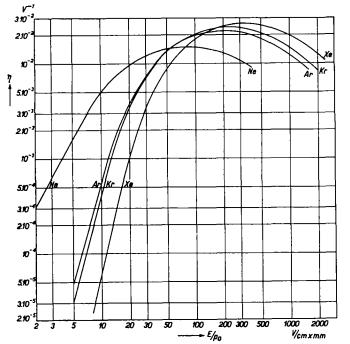
\includegraphics[width=\figurewidth,clip,trim={0 0 0 0},angle=0,origin=c]{Figures/GasTest/XenonPhysicsUseful/FirstTownsendCoefficientKruithof1960.jpg}
	\caption[The reduced first Townsend ionization coefficient $\eta \equiv \alpha / E$ for neon, argon, krypton, and xenon.]{The reduced first Townsend ionization coefficient $\eta \equiv \alpha / E$ for neon, argon, krypton, and xenon, from Ref.~\cite{Kruithof1940}.}
	\label{fig:first Townsend}
\end{figure}

The duration of the EL process is related electron drift velocity (v), which also depends on reduced electric field (E/n), as measured in Ref.~\cite{English1953, Bowe1960, Pack1962, Brooks1982, Berghofer2004}. In the range of \SIrange{5}{25}{\townsend},  a naive linear fit from Ref.~\cite{Brooks1982} shows in xenon, 
\begin{align}
v\ [\si{\mm\per\us}] \approx 0.556 E/n\ [\si{\townsend}] \label{eqn:xenon electron drift velocity}
\end{align}


Therefore, xenon is a good scintillation medium for its quantity of photon production and its transparency to these photons. With its well-characterized quantities, we chose it as the major operating medium for the ELD.



\begin{comment}
dead time: 185,212

eep: 55, 62, 256
Cherenkov radiation: 2, 51
muon (crossing EL region) : 107, 291,75, 
muon (anodic): 207
muon (cathodic): 7, 40 , 49
radiation
S1: 64, 210
anode cone: 47, (76,77), (175-177)
cathodic corner(or really close to cathode) :145, 67
EL region: 218,83
cathodic : 21,44
noise: 34
dark current: 53
PTFE fluo: 161(160),
ring radiation: 248, 181, 85, 105, 
grid radiation: 117
\end{comment}

\section{Signals}
\label{sec:events}
%An event  is the process that a particle interacts with the medium which then emit photons in the ELD. An event sometimes can be separated into sub-events, due to the time The study on the PMT photons pulses that we record from an event or a sub-event is the fundamental elements of the understanding of the detector performance, and leads to the understanding of the electron emission process. 
%Signals, PMT photon pulses that we record, are the fundamental elements of to understand detector activities. 
A variety of processes can give rise to signals in the detector. Based on their source origin, signals are separated to four different categories:
\begin{itemize}
	\item electron emission (both from the grid wires and from the grid rings)
	\item particle radiation from radioactive materials (both from inside and from outside the ELD),
	\item cosmic ray,
	\item and other miscellaneous sources, which include: 
	\begin{itemize}
		\item electronic noise %(from the electrical ground of the building and other powered devices, e.g. the KNF circulation pump.)
		\item PMT dark current, 
		\todo{\item PMT afterpulsing,}
		\item PTFE cone reflector fluorescence, 
		\item Cherenkov radiation (in PTFE cone reflectors and PMT windows)%(created in the PTFE cone reflectors and the PMT windows when a charge particle, most likely an electron or a muon, passes through),
		\item discharge, as in a short-lived plasma in the medium, i.e., breakdown.
	\end{itemize}
\end{itemize}

\subsection{Electron emission} 
\label{sec:events ee}
Electron emission signals, especially those from the grid wires, are our signals of interest. A cartoon of the physical process and an example waveform of \ees s are shown in Fig.~\ref{fig:ElectronEmissionPulse}. An electron leaves the cathodic electrode from various types of emission processes. After the electron left the wire surface, the high electric field around the cathodic wire will quickly energize the electron. The high energy electron then ionizes and excites the atoms around it. The process in which more drifted electrons are produced is called electron multiplication; since in this particular case, the electron multiplication process happens near the cathodic electrode, it is also called the cathodic gas gain. In the high electric field region around the cathodic wire, more EL light is produced per unit of time compared to a lower electric field region. This is the cause of the ``peak" at the beginning of the \ees .  Next, these electrons drift to the anodic electrode according to the voltage difference between the two grids, producing EL light along the drift. This process is responsible for the majority of EL light seen in the \ees . There is a clear start and stop time for the \ees . The time difference between the two times (\ees\ duration) is approximate to the duration of this drift. Then, drifted electrons get close to the high electric field region around the anodic electrode. Because of  the high electric field, drifted electrons also go through a similar electron multiplication process in this high electric field region, which is also called the anodic gas gain. This process also creates more electrons and a higher production rate of EL light, resulting in a ``peak" at the ending of the \ees . The peak at the end of the signal is lower than the peak at the beginning of the signal. This is resulting from the dispersion of the arrival times of drifted electrons on anodic electrode, because the different microscopic trajectory each drifted electron takes to reach the anodic electrode. The different arrival times of the drifted electrons cause the final increment of EL light production from different electrons do not happen coincidently. This lowers the height of the peak at the ending of the \ees . Another reason for the difference in height of the peaks is because the electric field on the anodic wire is smaller than that of cathodic wire with regard to the wire diameter of the anodic wire are larger, which therefore results in a smaller production of EL light.

\begin{figure}[!htbp]
	\centering
	\begin{subfigure}[b]{\figurewidth}
		\centering
		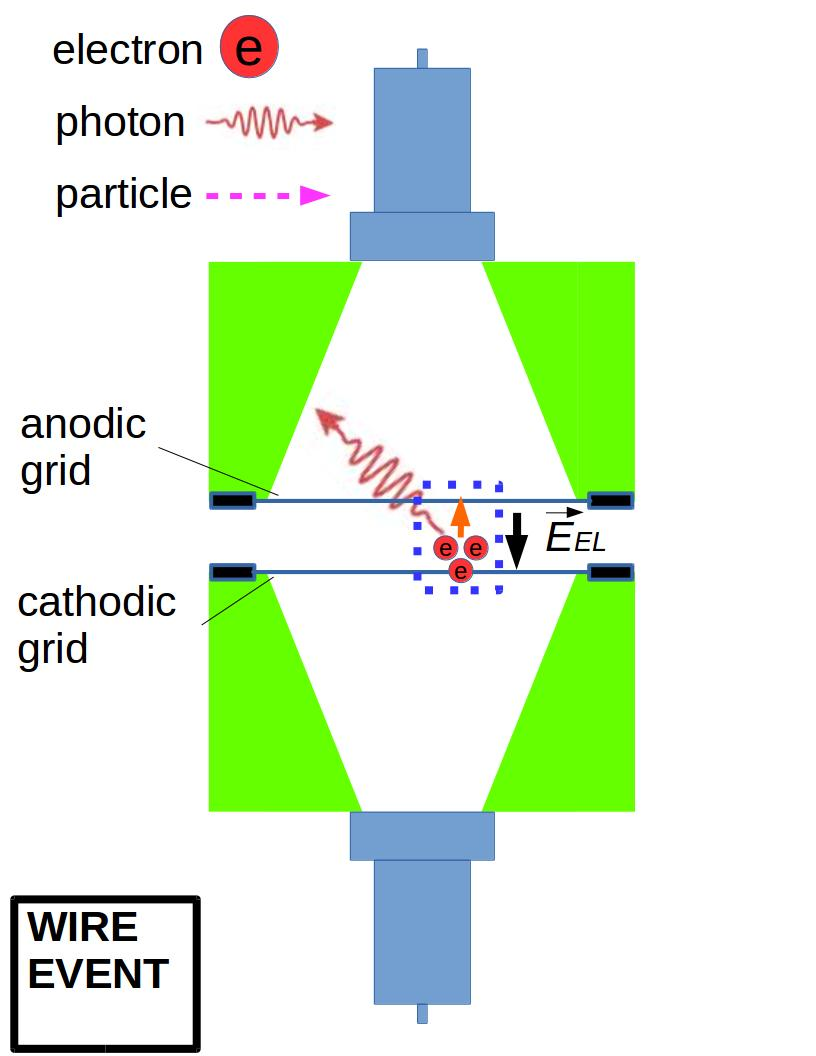
\includegraphics[width=\halfwidth,clip,trim={0 0 0 0},angle=0,origin=c]{Figures/GasTest/WeiDrawEvent/WirePhotoF.jpg}
%		\caption{}
%		\label{fig:ElectronEmissionPulse a}
%	\end{subfigure}
%	\begin{subfigure}[b]{\halfwidth}
%		\centering
	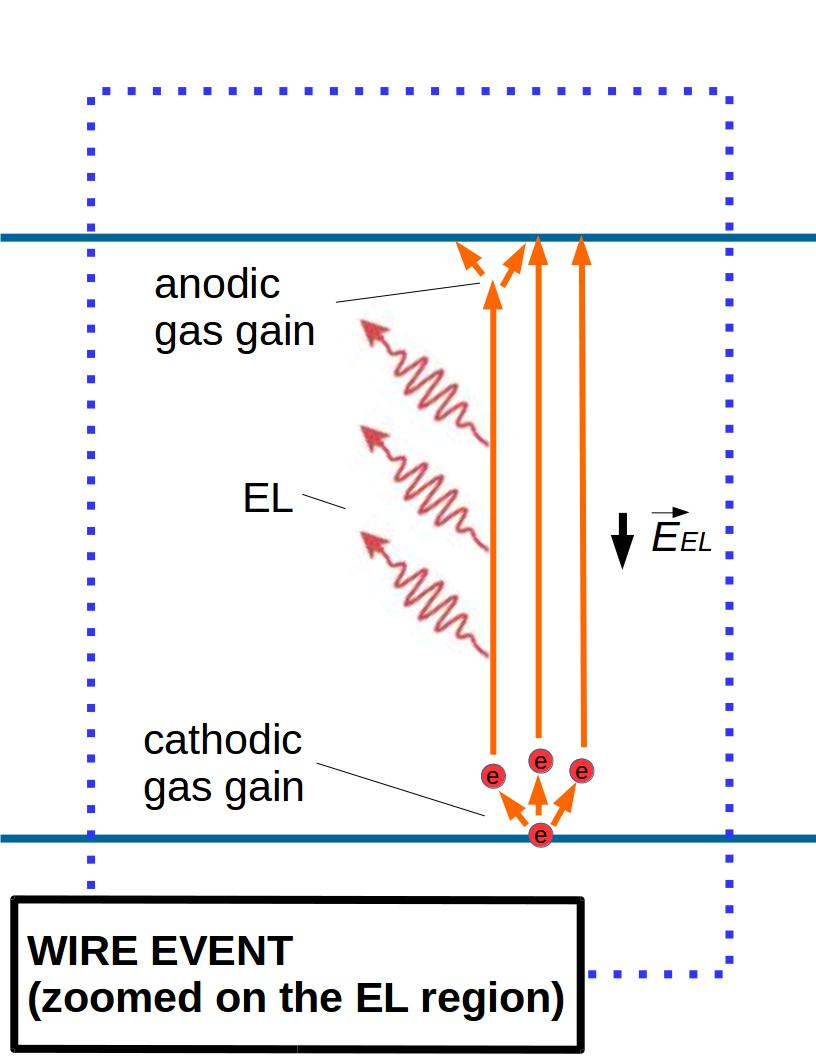
\includegraphics[width=\halfwidth,clip,trim={0 0 0 0}]{Figures/GasTest/WeiDrawEvent/WirePhotoZ.jpg}
		\caption{}
		\label{fig:ElectronEmissionPulse b}
	\end{subfigure}
    \par\bigskip
	\begin{subfigure}[b]{0.8\textwidth}
	\centering
	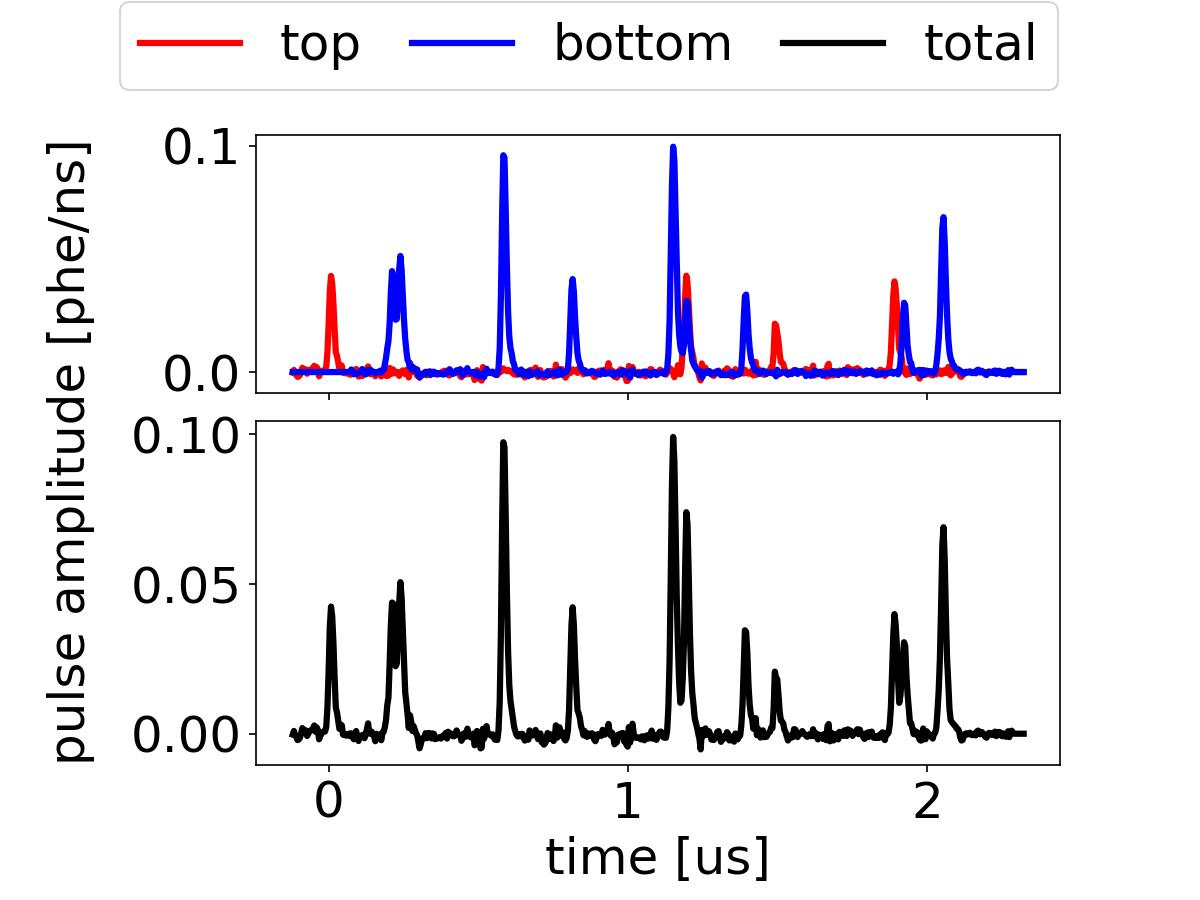
\includegraphics[width=\figurewidth,clip,trim={0 0 0 0}]{Figures/GasTest/exampleWaveforms/proc64767id00000197.jpg}%062
	\caption{}
	\label{fig:ElectronEmissionPulse c}
\end{subfigure}
	\caption[\gtest\ electron emission event from grid wires]{\gtest\ electron emission event from grid wires. (a) Cartoon of the process. (b) An example waveform. Data were taken at \ddtt{2017}{12}{08}{14}{02}, with \opvtvb\ at \SIlist{+6;-6}{kV}, \opgd\ at \standarddensity . See text for details.}
	\label{fig:ElectronEmissionPulse}
\end{figure}

Of the features described above, the most important features of  the \ees\ is the EL duration. The other signal shape features, such as the early and late gas gain peaks, are not apparent because the light collection efficiency is not high enough. The EL duration is approximately equal to the duration of electron drift between the two electrodes. The deviation of electric field between the two electrode is much smaller than its average value. Therefore, the drift duration can be roughly estimated by, 

\begin{align}
\text{drift duration} = \frac{\text{distance between two electrodes}}{\text{drift velocity at the average electric field between two electrodes} }
\end{align}

The other important feature of the \ees\ is the quantity of its EL production. EL light production in the major part of \ees\ is uniform, except for at the beginning and at the ending of the signal, because the deviation of the drift electric field is small. Since the electron multiplication around the cathodic wires happens early in the process before the major EL light production, the total counts of photons created in an \ees\  can be estimated as,
\begin{align}
\#\ \text{EL photons} & \approx \#\ \text{EL photons per drifted electron} \times \text{cathodic gas gain}
\end{align}
where the number of EL photons per drifted electron and the cathodic gas gain are estimated below.

The number of EL photons per drifted electron and the cathodic gas gain are related to the reduced electric field in the EL region and surface reduced electric field on the cathodic wire. The value of both reduced electric field can be derived from the gas density and the electric field, which can be estimated from the voltages, wire diameters and the distances between two wires of the two grids. The electrostatic solution of the electric field in the ELD is solved by COMSOL, as described in Appendix~\ref{chapter:field}. The results of the electric fields in the EL region (drift fields) and the average surface electric fields vs. \opdv\ are shown in Fig.~\ref{fig:surface electric field dV}.  The woven pattern of the grid cause that the surface electric field in the middle of the wire between two woven knots are higher than average by \SI{\sim 16}{\percent}, which is also discussed in Appendix~\ref{chapter:field}. The average number of photon production per EL distance is a known function of reduced electric field, as discussed in Section~\ref{sec:gtest light procduction}.% and its values at different \opgd\ and \opdv\ are shown in Fig.~\ref{fig:photon per drifted electron}. 
\begin{figure}[!htbp]
	\centering
	\begin{subfigure}[b]{0.8\textwidth}
		\centering
		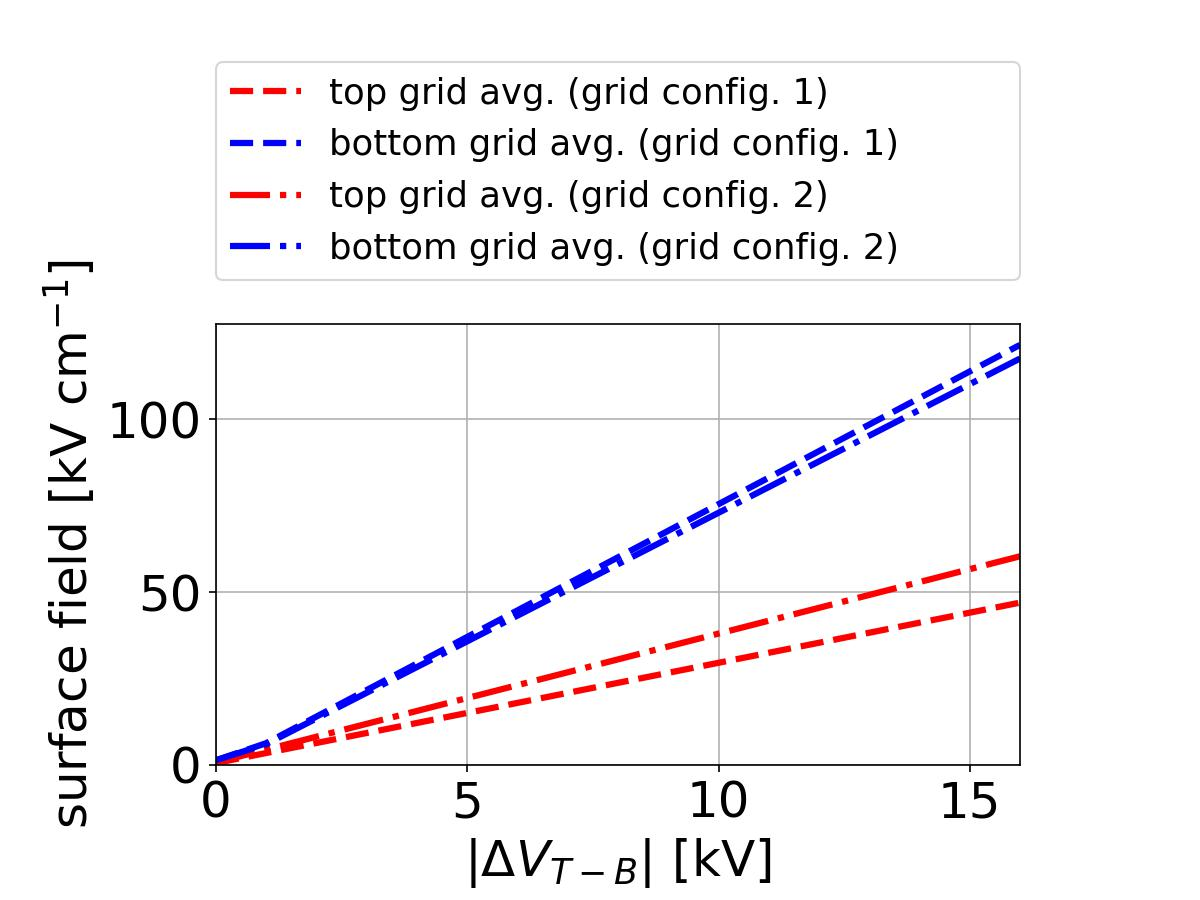
\includegraphics[width=\figurewidth,clip,trim={0 0 0 0},angle=0,origin=c]{Figures/GasTest/ElectricField/SurfaceElectricFieldGas.jpg}
		\caption[]{}
		\label{fig:surface electric field dV}
	\end{subfigure}
	\par\bigskip
	\begin{subfigure}[b]{0.8\textwidth}
		\centering
		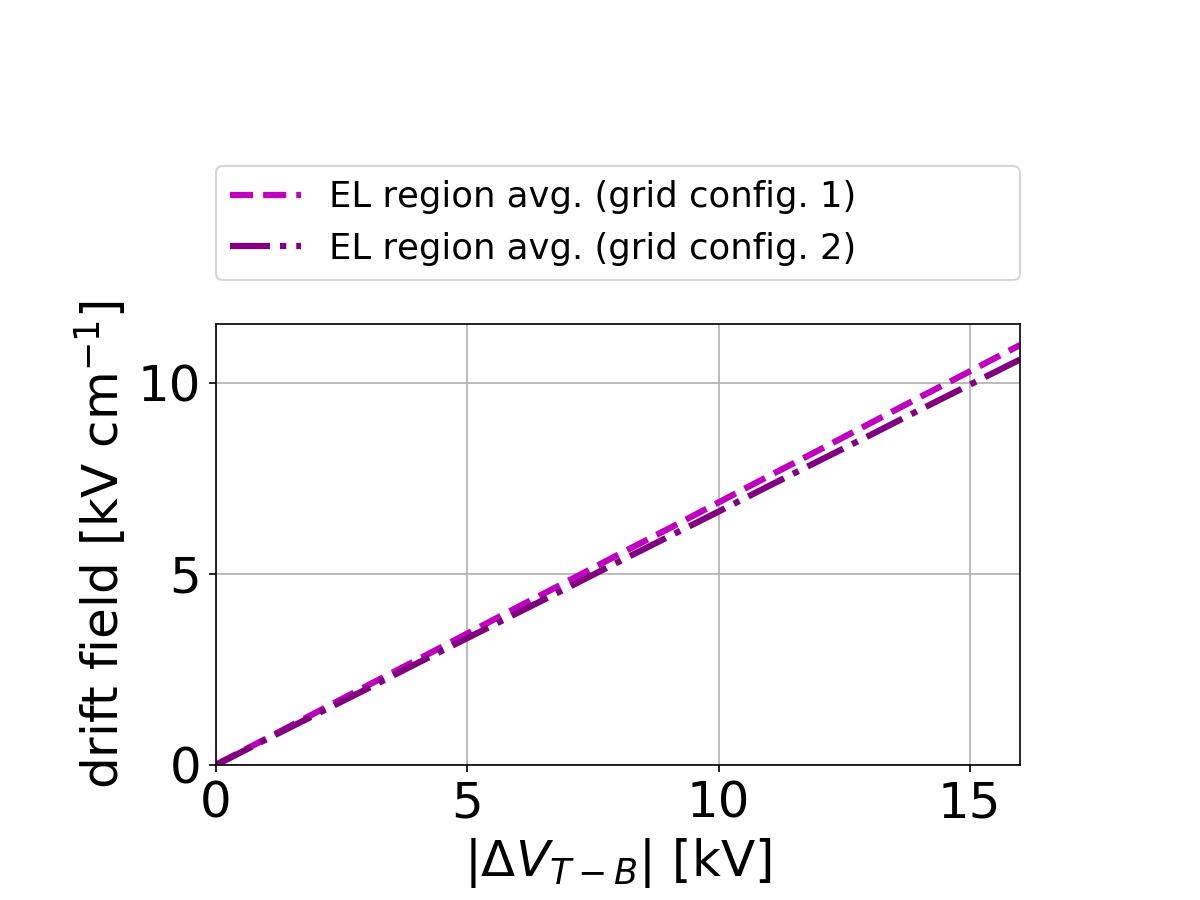
\includegraphics[width=\figurewidth,clip,trim={0 0 0 0}]{Figures/GasTest/ElectricField/DriftElectricFieldGas.jpg}
		\caption{}
		\label{fig:drift electric field dV}
	\end{subfigure}
	\caption[\gtest\ detector electric field.]{\gtest\ detector electric field. (a) \gtest\ wire surface electric field vs. \opdv\ for the top and bottom grid in different grid configurations. (b) \gtest\ EL region drift electric field vs. \opdv\ in different grid configurations.}
	\label{fig:gtest electric field}
\end{figure} %code in /Users/weiji/Google Drive/gastest/ElectricField

With the known surface reduced electric field, electron multiplication (cathodic gas gain) is studied using gas simulation softwares. A simple geometry is build and meshed in GMSH, as described in Ref.~\cite{Geuzaine2009}.  This software is capable of defining 3D finite element mesh, which interfaces with softwares like ElmerSolver and Garfield++ to solve the electric field in a defined geometry. Fig.~\ref{fig:electron multiplication sim geo} shows the defined geometry. This geometry includes a thin cylindrical surface in the center representing the grid wire as the surface emitting electrons, and a thick cylindrical surface outside representing the cut-off distance of electron multiplication. This cut-off distance is chosen to be sufficiently long so that the electric field beyond this distance is too small to allow most of the electron multiplication. The diameter of the two cylinders are \SI{75}{\um} and \SI{1}{\cm}. Voltages are assigned to two cylinders to create a chosen electric field on the surface of the wire. Next, the electric field map in this full geometry is solved by Elmer, as described in Ref.~\cite{Elmergrid2000, Kotila1999}.  Then, the gas simulation under such electric field map is done with Magboltz in Garfield++ interface, as described in Ref.~\cite{Biagi1999, Veenhof1998}. These softwares implement light yield and charge yield, also known as the photon and electron production, for electrons moving in a gas medium as a function of reduced electron field. By including the electric field map and choosing the corrects gas density, these softwares are able to simulate the photon and electron production with an electron that initiate from the wire surface. 

An example of electron multiplication simulation in the simple geometry is shown in Fig:~\ref{fig:electron multiplication sim result}. As the electron moves further away from the wire surface, both light production and electron production reduce. Results of the counts of electron multiplication vs. surface electric field at different gas density is shown in Fig.~\ref{fig:electron multiplication}. The number of collected EL photons of the \ees\ signals are shown in Fig.~\ref{fig:photon per electron sim}. Together with the EL duration, this number of collected EL photons are the important features of \ees\ signals that we used in the signal classification.
%Light collection of created photons also influence the total counts and duration of \ees . The approximately \SI{2}{\percent} light collection efficiency in the ELD results in only a portion of EL photons are seen by the PMTs. It causes the waveform of an \ees\ more coarsely distributed in time. This low number of collected photons also increases the difficulty of estimating the real EL duration.

\begin{figure}[!htbp]
	\centering
	\begin{subfigure}[b]{0.45\textwidth}
		\centering
		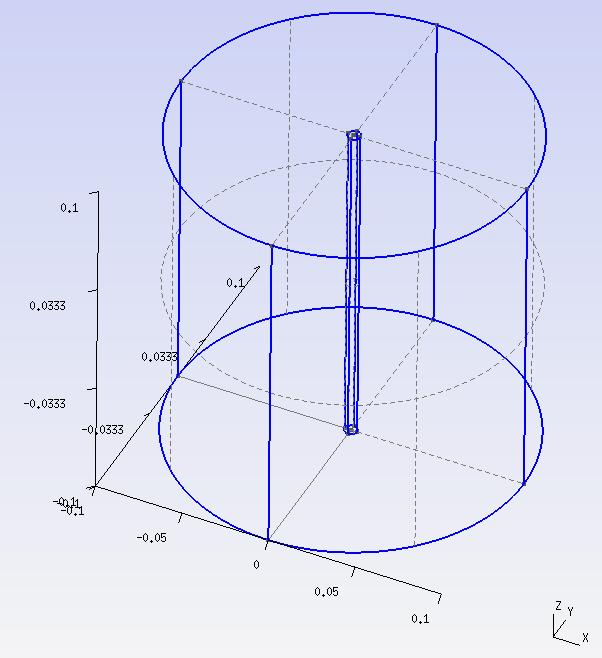
\includegraphics[width=\figurewidth,clip,trim={0 0 0 0}]{Figures/GasTest/GarfieldResults/SingleWireGeoPlus.jpg}
		\caption{}
		\label{fig:electron multiplication sim geo}
	\end{subfigure}
	\par\bigskip
	\begin{subfigure}[b]{\figurewidth}
		\centering
		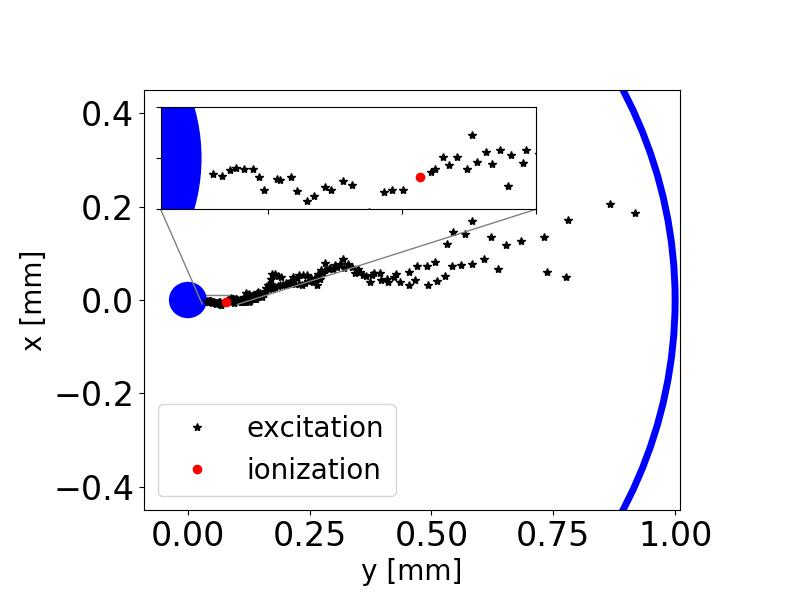
\includegraphics[width=\halfwidth,clip,trim={20 0 70 0}]{Figures/GasTest/GarfieldResults/GarOneEvent100.jpg}
		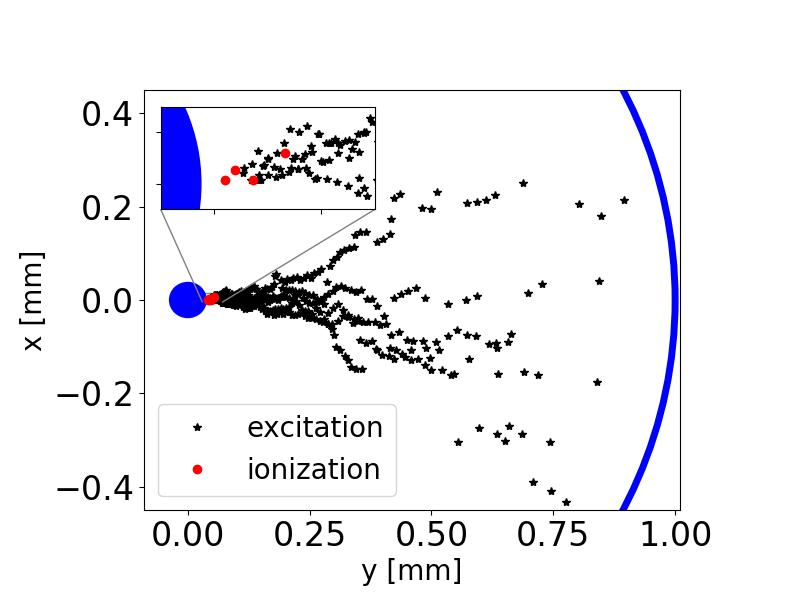
\includegraphics[width=\halfwidth,clip,trim={20 0 70 0}]{Figures/GasTest/GarfieldResults/GarOneEvent101.jpg}
		\caption{}
		\label{fig:electron multiplication sim result}
	\end{subfigure}
	\caption[A 3D simulation of an electron drifting in an axially symmetric electric field in xenon gas.]{A 3D simulation of an electron drifting in an axial symmetric electric field in xenon gas. (a) Geometry defined in GMSH (unit in \si{\cm}) \cite{Geuzaine2009}. Electrons are emitted at one point from the wire in the center. (b) Example simulation results, which is taken at \opgd\ \SI{0.137}{\mole\per\liter} (T = \SI{295}{\kelvin}, P = \SI{3.3}{\bara}), showing the excitation and ionization sites. The blue curves are the boundary of the outer edge of simulation (diameter : \SI{2}{\mm}) and  the wire surface (diameter: \SI{75e-3}{\mm}). Left: a simulated event with a single ionization site. Right: a simulated event with four ionization sites. This simulation is conducted with Elmer and Garfield++, as described in Ref.~\cite{Elmergrid2000, Kotila1999, Biagi1999, Veenhof1998}.}
	\label{fig:electron multiplication sim}
\end{figure}

\begin{figure}[!htbp]
	\centering
	\begin{subfigure}[b]{0.7\textwidth}
		\centering
		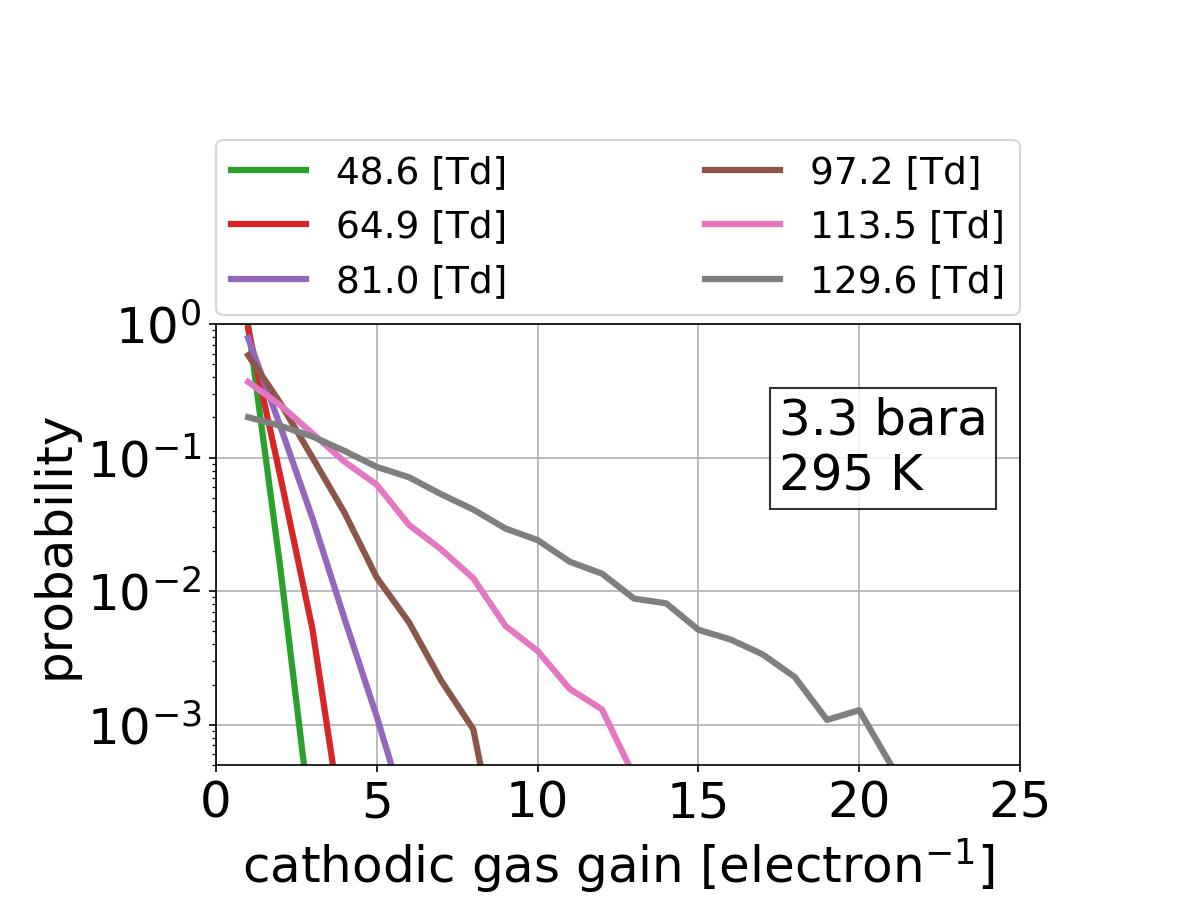
\includegraphics[width=\figurewidth,clip,trim={0 0 0 0}]{Figures/GasTest/xenonProperties/PhotonMultiplicationNaiveReduced.jpg}
		\caption{}
		\label{fig:electron multiplication ind}
	\end{subfigure}
%	\par\bigskip
	\begin{subfigure}[b]{0.7\textwidth}
		\centering
		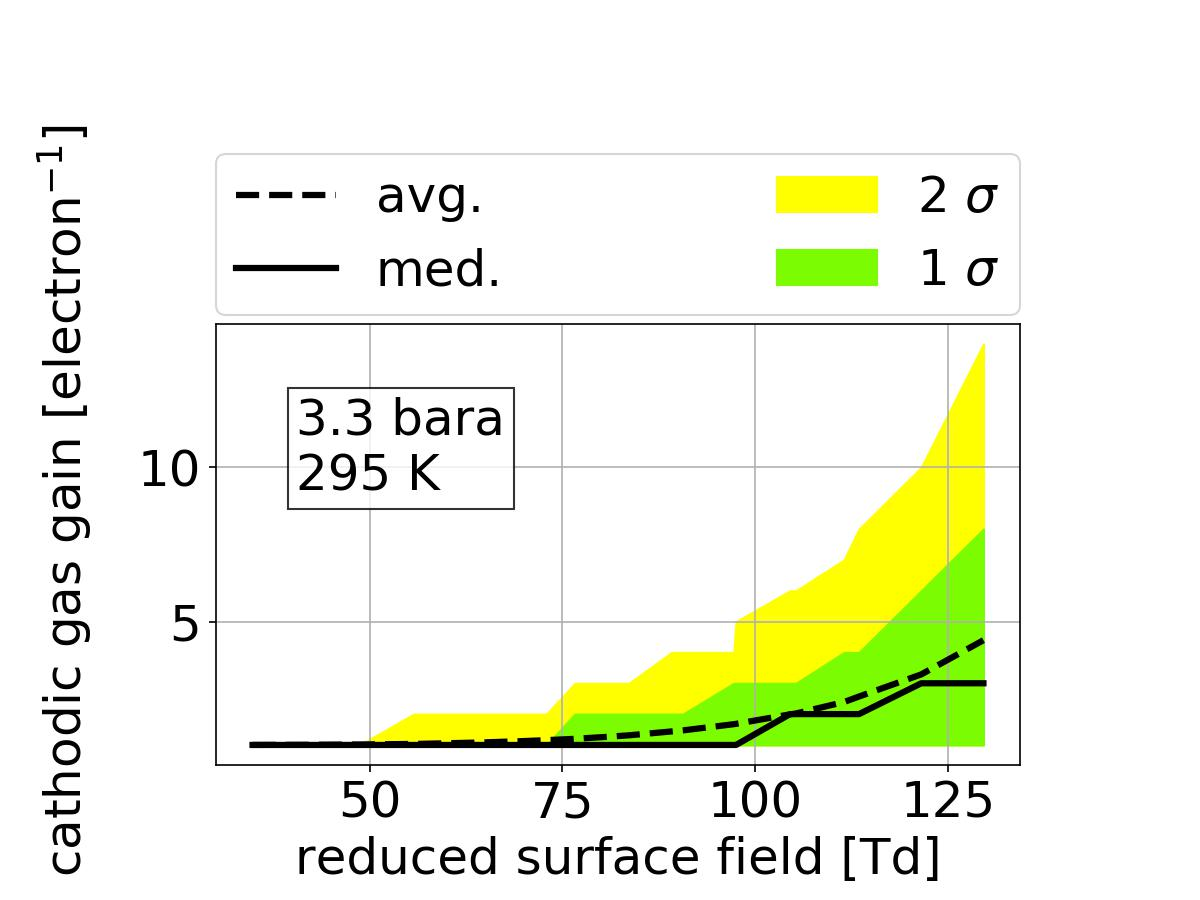
\includegraphics[width=\figurewidth,clip,trim={0 0 0 0}]{Figures/GasTest/xenonProperties/MultiplicationMeanSigma3300mbarReduced.jpg}
		\caption{}
		\label{fig:electron multiplication para}
	\end{subfigure}
	\caption[Simulated cathodic electron gas gain vs. reduced surface electric field.]{Simulated cathodic electron gas gain vs. reduced surface electric field. (a) Simulated cathodic gas gain probability distribution in different reduced surface electric fields. (b) The average, median, \onesigma\ band (\SIrange{15.9}{84.1}{\percent}), and \twosigma\ band (\SIrange{2.3}{97.7}{\percent}) of cathodic gas gain vs. the reduced surface electric field. Simulation is taken at \opgd\ \SI{0.137}{\mole\per\liter} (T = \SI{295}{\kelvin}, P = \SI{3.3}{\bara}).}
	\label{fig:electron multiplication}
\end{figure}% code in '/Users/weiji/Google Drive/gastest/xenonProperties/xenonIonization.py'

\begin{figure}[!htbp]
	\centering
	\begin{subfigure}[b]{0.7\textwidth}
		\centering
		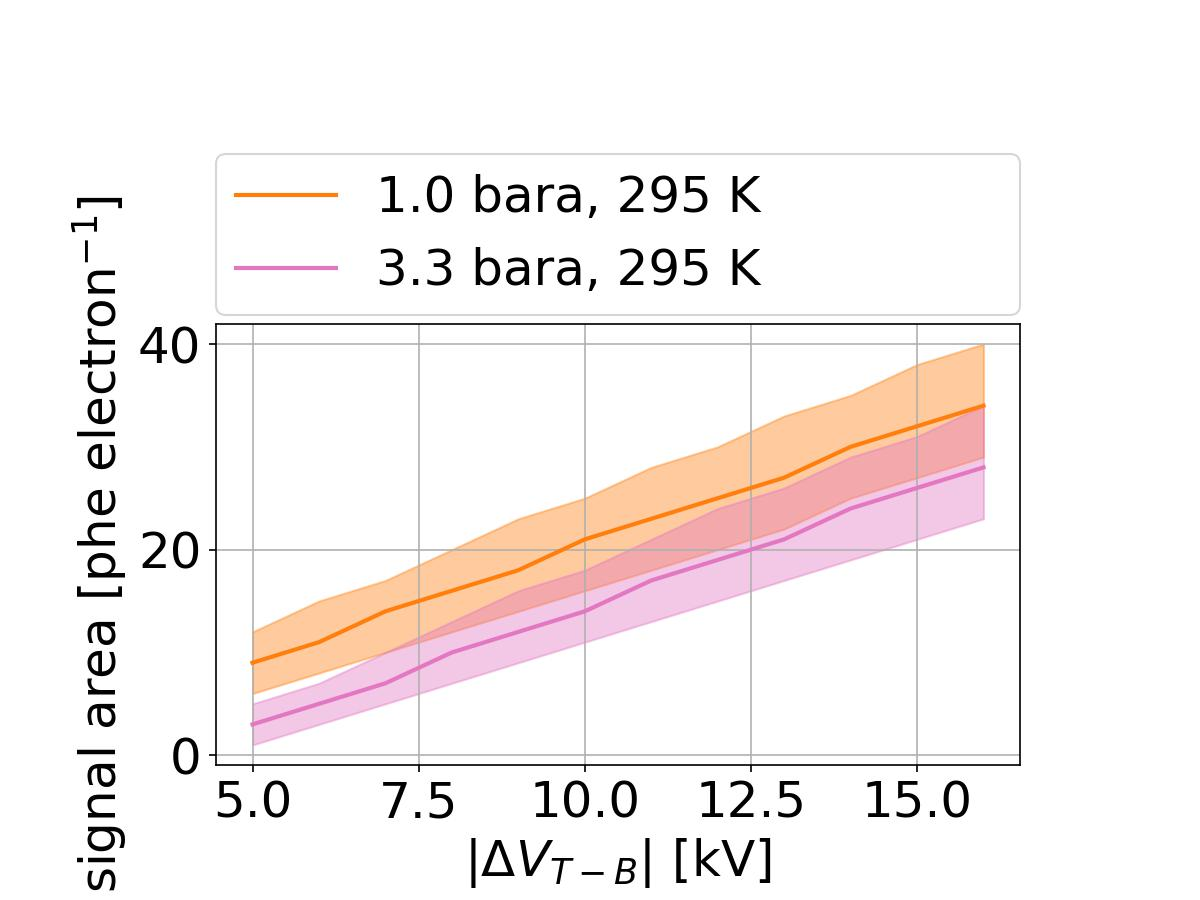
\includegraphics[width=\figurewidth,clip,trim={0 0 0 0}]{Figures/GasTest/xenonProperties/MultiplicationPhotonCollectionNaiveProfileMeanSigma3300mbarPerDriftElecton.jpg}
		\caption{}
		\label{fig:photon per drifted electron }
	\end{subfigure}
%	\par\bigskip
	\begin{subfigure}[b]{0.7\textwidth}
		\centering
		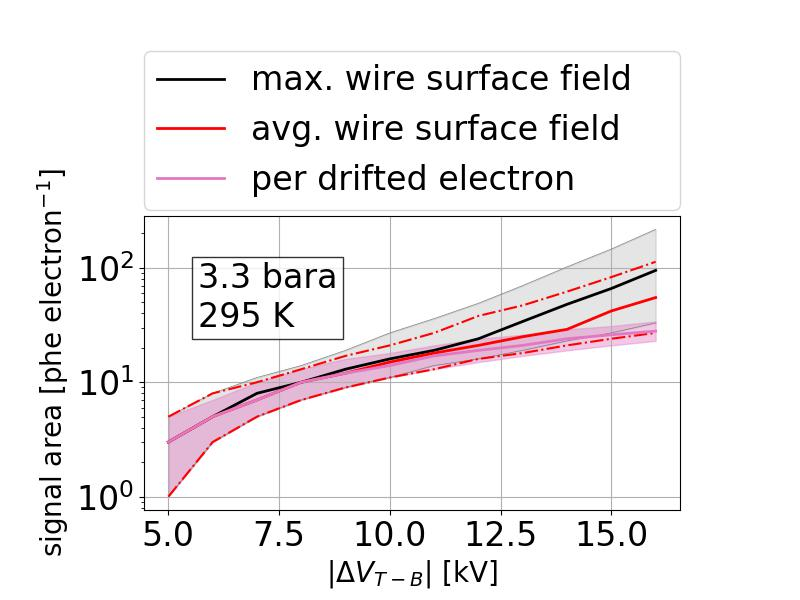
\includegraphics[width=\figurewidth,clip,trim={0 0 0 0}]{Figures/GasTest/xenonProperties/MultiplicationPhotonCollectionNaiveProfileMeanSigma3300mbar.jpg}
		\caption{}
		\label{fig:photon per electron}
	\end{subfigure}
	\caption[Simulated signal areas vs. \opdv .]{Simulated signal areas vs. \opdv . (a) Simulated signal area of a single drifted electron from the bottom grid at different gas densities. (b) Simulated signal area of an electron generated at different locations on the bottom grid. The black line corresponds to locations with maximum electric field on the grid. The red line corresponds to locations with average electric field on the grid. The green line shows the simulated signal area of a single drifted electron. Simulation is taken at \opgd\ \SI{0.137}{\mole\per\liter} (T = \SI{295}{\kelvin}, P = \SI{3.3}{\bara}). The solid lines are the medians. The dashed lines, color shaded bands are \onesigma\ bands (\SIrange{15.9}{84.1}{\percent}), respectively.}
	\label{fig:photon per electron sim}
\end{figure}% code in '/Users/weiji/Google Drive/gastest/xenonProperties/xenonIonization.py'

Therefore, \ees s  have a known EL duration and EL photons production dependence on the detector \opgd\ and \opdv . We use these two important characteristics of signals to distinguish \ees s in the future signal classification.

\subsection{Particle radiation}
\label{sec:events particle}
Particle radiation is the high energy particle originating from radioactive decay of unstable atoms in materials inside and outside the detector. The high energy particle enter the detector and deposit energy there through different processes. A high energy photon (gamma radiation) loses energy through thermal elastic scattering, photoelectric process, Compton scattering, and other particle energy loss processes; A high energy charged particle, e.g. electron (beta radiation), \ce{^{4}_{2}He} (alpha radiation), predominately loses it energy through ionizing atoms in detector materials, as described in Ref.~\cite{Blum2008}.  These processes produce excited xenon atoms and free electrons, which later produce primary scintillation and EL photons. The primary scintillation photons (S1) are collected and seen immediately. The EL photons, on the other hand, resulting from electrons drifting in the high electric field region in the detector, are usually produced later. 

A high energy gamma event can enter the ELD since its energy loss in detector skin materials is small. The photon attenuation length, which characterizes how far a photon can go, usually decrease as we have denser materials, higher average atomic mass in the materials, and lower incident particle energy. The photon attenuation length in xenon is shown in Fig.~\ref{fig:xenon photon attenuation}. Along photon attenuation, high energy electrons can be produced from gamma radiation through some kind of energy loss process, like Compton scattering, Auger electron emission. These high energy electrons can be produced inside the ELD, deposit its energy, and raise signals in the detector. The energy deposition length depends on the material, especially its density and its average atomic mass, and the energy of the incident particle. Similar to the photon attenuation process, denser material, higher average atomic mass, and lower incident particle energy usually results in smaller energy deposition length. The energy deposition length in xenon is shown in Fig.~\ref{fig:xenon electron range}. For an electron with energy in the range of \SIrange{10}{1000}{\keV}, which is the common energy for beta radiation, the continuous slowing down approximation range (CSDA range), also know as the average path length traveled by the charged particle (electron), is in the range of \SIrange{6e-4}{1}{\gram\per\cm\squared}, corresponding to \SIrange{1e-5}{2.e-2}{\cm} with xenon gas density at \standarddensity\ (\SI{18.0e-3}{\gram\per\cm\cubed}). %This energy deposition length is smaller compared to the height of the EL region, indicating low possibility for distinguishing the by arrival time of the secondary electrons.
The number of free ionization electrons in this event is associated with the energy-loss of the incident particle. During the measurement, a population associated with xenon K shell X-ray ($K_{\alpha}$: \SI{29.8}{\keV}, $K_{\beta}$: \SI{33.6}{\keV}, from Ref.~\cite{Dulieu2007, TabRadv8}) is observed to be one of the byproduct of particle radiation energy loss process, confirming that this type of signal is associated with external radiation.

\begin{figure}[!htbp]
	\centering
	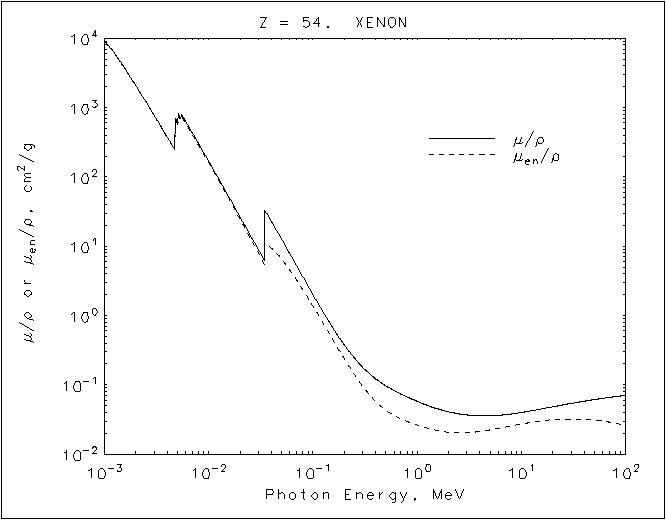
\includegraphics[width=.7\textwidth,clip,trim={0 0 0 0},angle=0,origin=c]{Figures/GasTest/XenonPhysicsUseful/PhotonAttenuation.jpg}
	\caption[Attenuation length of photon in xenon.]{Attenuation length of photon in xenon, from Ref.~\ref{NIST,}.}
	\label{fig:xenon photon attenuation}
\end{figure}

\begin{figure}[!htbp]
	\centering
	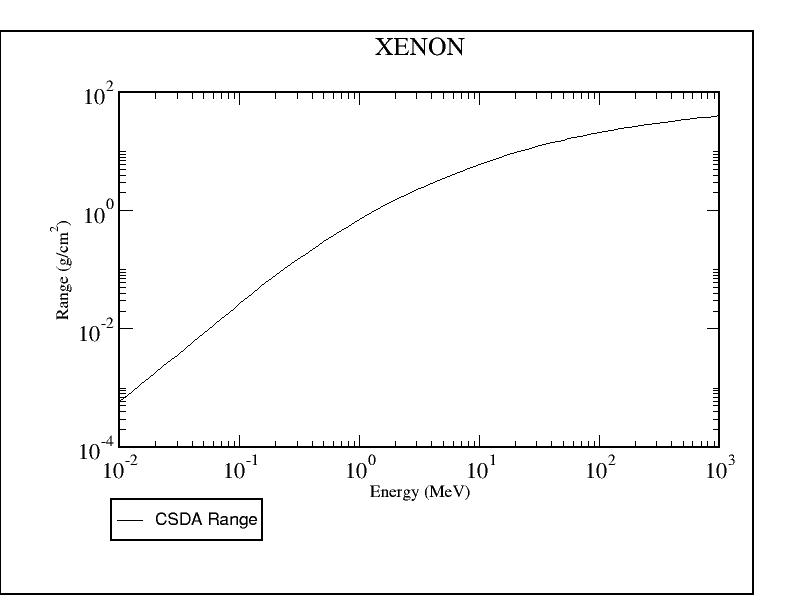
\includegraphics[width=.7\textwidth,clip,trim={0 0 0 0},angle=0,origin=c]{Figures/GasTest/XenonPhysicsUseful/ElectronRange.jpg}
	\caption[CSDA range of electrons in xenon.]{CSDA range of electrons in xenon, from Ref.~\ref{NIST, ESTAR}.}
	\label{fig:xenon electron range}
\end{figure}

A high energy external beta radiation, however, is less likely to enter the ELD compared to high energy gamma radiation because the beta radiation penetration length (approximate to the material CDSA range) is shorter than gamma radiation. Since the electron CDSA range is small compared to the thickness of xenon gas skin outside the ELD, with addition stopping power from dense PTFE reflector cone, the beta radiation would be stopped before it enters the ELD. 

According to the location of energy deposition site, the high energy particle from radiation produce different look of signals, which will be discussed separately.

\paragraph{Anode cone event} 
\label{sec:events particle anode cone}
Anode cone events are the particle radiation events which have energy deposition location in the PTFE reflector cone close to the anodic grid side (anode cone). A cartoon of the physical process and an example waveform of anode cone event, as well as two zoomed plots of the waveform in different parts of the process, are shown in Fig.~\ref{fig:anode cone}. The cartoon part A in Fig.~\ref{fig:anode cone a} shows an external particle entering the anode cone region and deposit energy there. This process produce scintillation photons, the signal of which are collected and seen immediately, shown in Fig.~\ref{fig:anode cone d}. The primary scintillation signal normally has a TBA (top-bottom asymmetry) heavier in the anode side PMT than the cathode side, indicating this photon signal is produced in the anode cone (top cone in this case). The free electrons drift to the anodic grid according to the electric field in the anode cone . Even though the electric field in the cone region is too small to produce large quantity of EL light during electron drift, when these electrons get close to the anodic grid wire, the electric field around the anodic grid wires are big enough to produce EL light. This is the source of the secondary photon signal, which follows the preceding signal after the amount of time that it took electron to drift. The cartoon part B in Fig.~\ref{fig:anode cone b} shows this process, and Fig.~\ref{fig:anode cone e} shows the corresponding part of the signal. The pulse shape of the secondary photon signals has a comparably slower rising and falling edge at the beginning and the ending of it. It also has a higher TBA because EL around the anode wire primarily happens above the anodic wire. The bottom PMT is in the shadow of grid wires when the top PMT is not. This difference causes a ratio of \num{\sim 2} increment on light collection ratio between the top PMT and the bottom PMT. These characteristic signatures are useful for veto large-area anode cone events. However, when their signal area get smaller (probably because of a lower energy deposition of external particles), it becomes difficult to find these signals by their shape. Therefore, a signal selection based on preceding signal is conducted to find the secondary signal from the primary scintillation signal. The time separation between these two signal is estimated by the known measured electron drift velocity in gaseous xenon, as described in Ref.~\ref{English1953, Brooks1982}. Electron drift velocity in gaseous xenon is approximately \SI{0.556}{\mm\per\us\per\townsend} E/N for reduced electric field (E/N) in the range of \SIrange{5}{25}{\townsend}. The maximum separation time for this detector at xenon gas density \standarddensity , \opvt\ in the range of \SIrange{+4}{+8}{\kV} is approximately \SIrange{85}{75}{\us}. The value of this maximum separation time decreases as decreasing the operation pressure in the detector. The value of maximum separation time drives the choice of \SI{100}{\us} preceding signal selections of this type of signals.  

\begin{figure}[!htbp]
	\centering
	\begin{subfigure}[b]{0.8\textwidth}
		\centering
		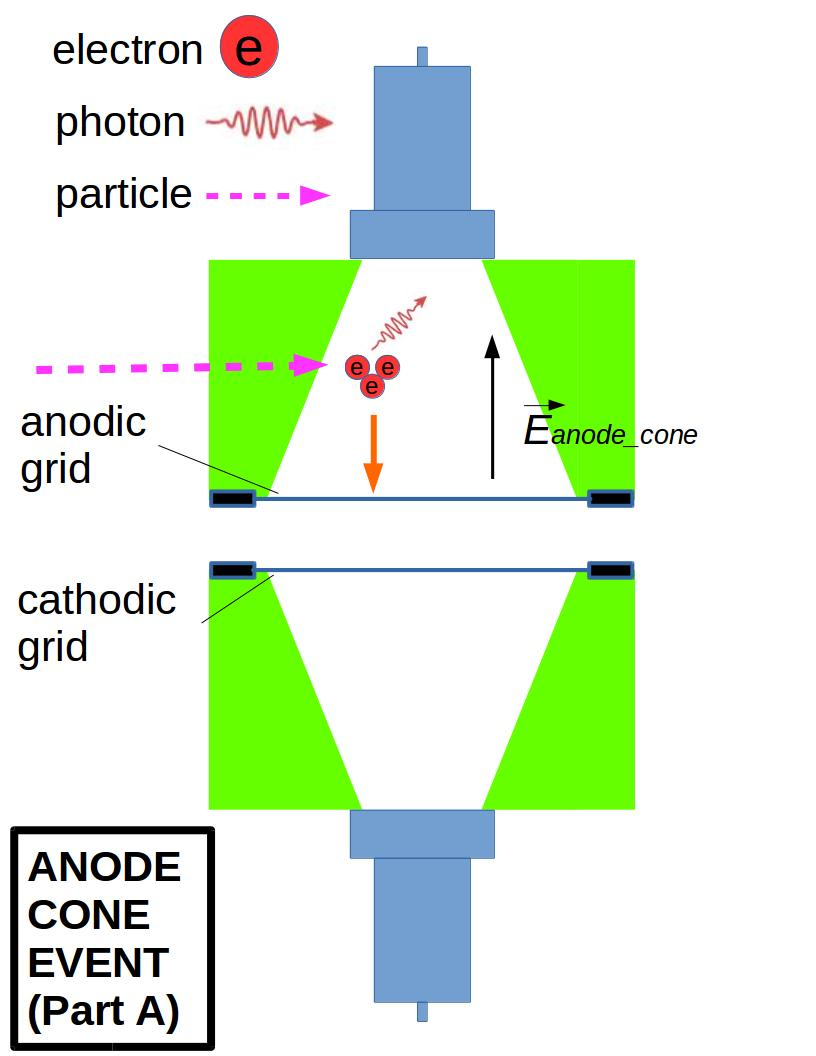
\includegraphics[width=\halfwidth,clip,trim={0 0 0 0},angle=0,origin=c]{Figures/GasTest/WeiDrawEvent/AboveAnoA.jpg}
%		\caption{}
%		\label{fig:anode cone a}
%	\end{subfigure}
%	\begin{subfigure}[b]{\halfwidth}
%		\centering
		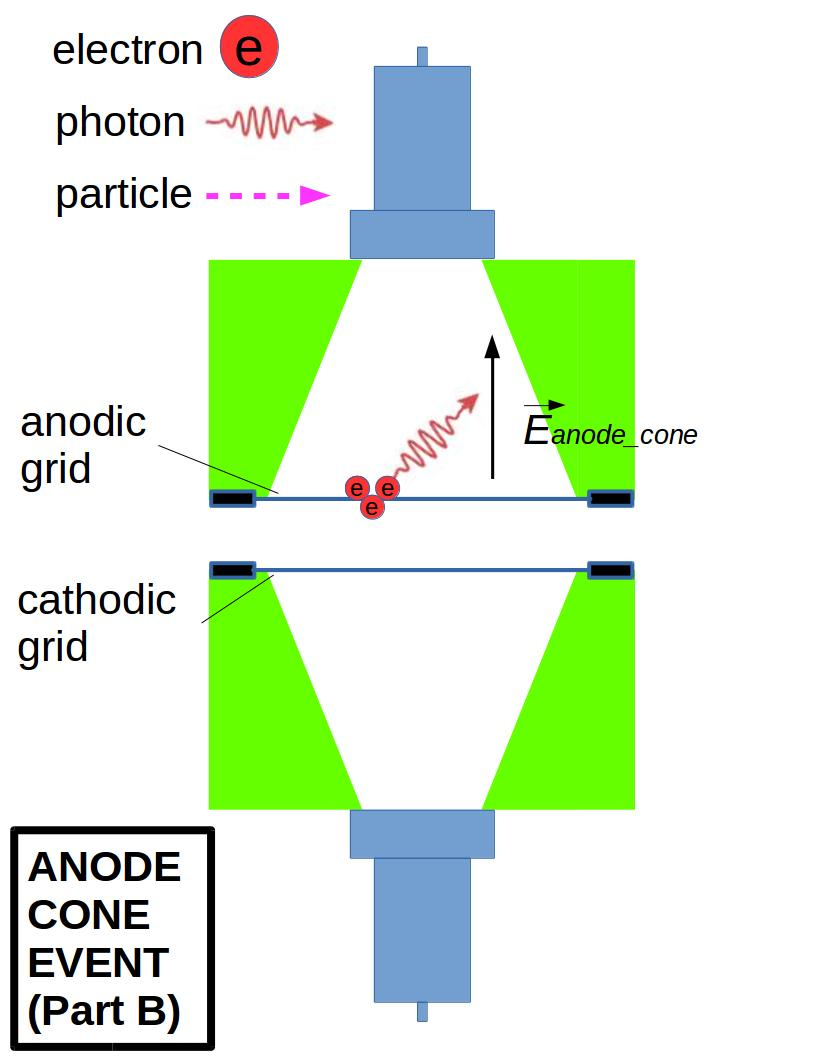
\includegraphics[width=\halfwidth,clip,trim={0 0 0 0}]{Figures/GasTest/WeiDrawEvent/AboveAnoB.jpg}
		\caption{}
		\label{fig:anode cone b}
	\end{subfigure}
	\par\bigskip
	\begin{subfigure}[b]{0.7\textwidth}
		\centering
		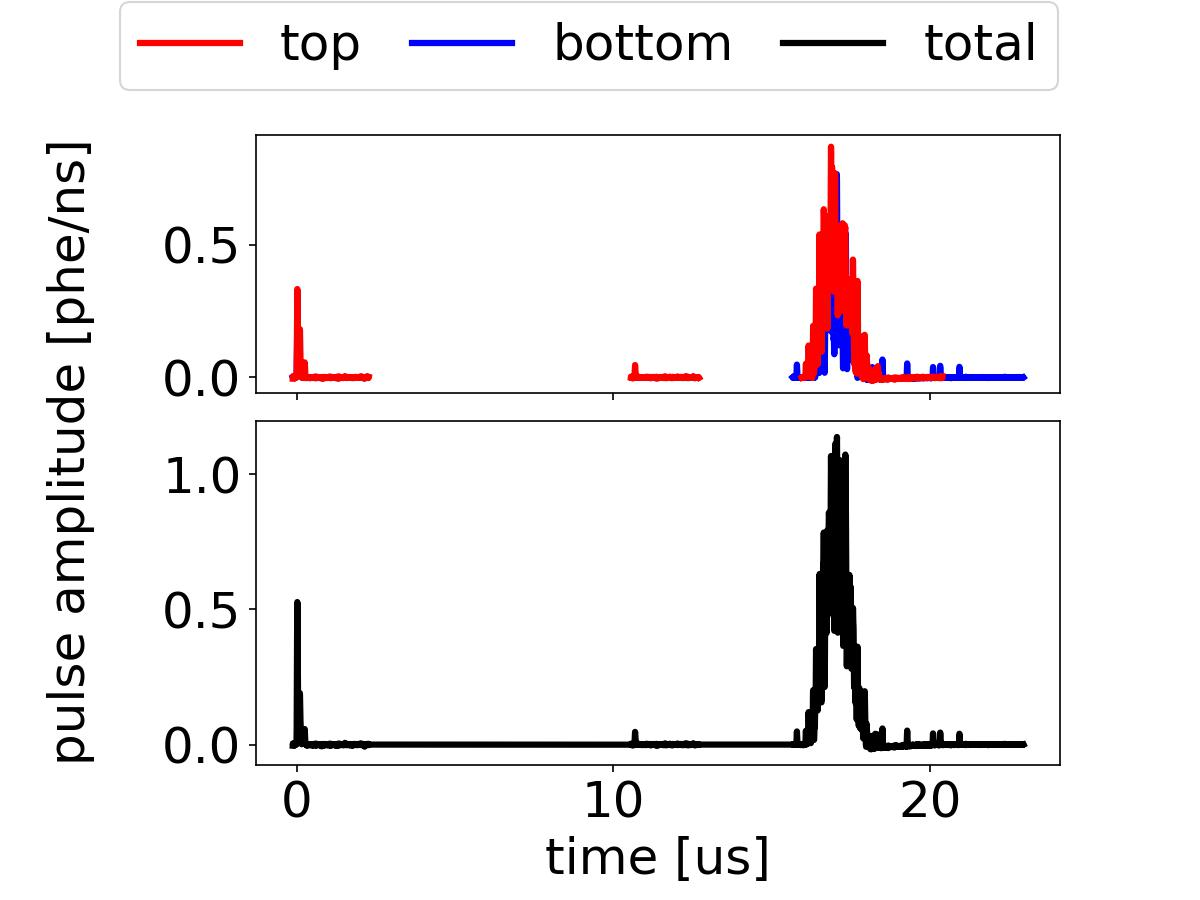
\includegraphics[width=\figurewidth,clip,trim={0 0 0 0}]{Figures/GasTest/exampleWaveforms/proc64767AnodeCone1.jpg}
		%{Figures/GasTest/exampleWaveforms/proc64767id00000047.jpg}
		\caption{}
		\label{fig:anode cone c}
	\end{subfigure}
	\caption[\gtest\ signal: anode cone event.]{\gtest\ signal: anode cone event. (a) Cartoon of the process. Left: Primary scintillation light  ionization electrons are produced from the particle interaction, and the ionization electrons drift to the anodic grid (part A). Right: EL light is produced in the high electric field region around the anodic grid wires (part B). (b) An example waveform of an anode cone event. Data were taken at \ddtt{2017}{12}{08}{14}{02}, with \opvtvb\ at \SIlist{+6;-6}{kV}, \opgd\ at \standarddensity .}
	\label{fig:anode cone}
\end{figure}

\begin{figure}[!htbp]\ContinuedFloat
	\centering
	\begin{subfigure}[b]{0.7\textwidth}
		\centering
		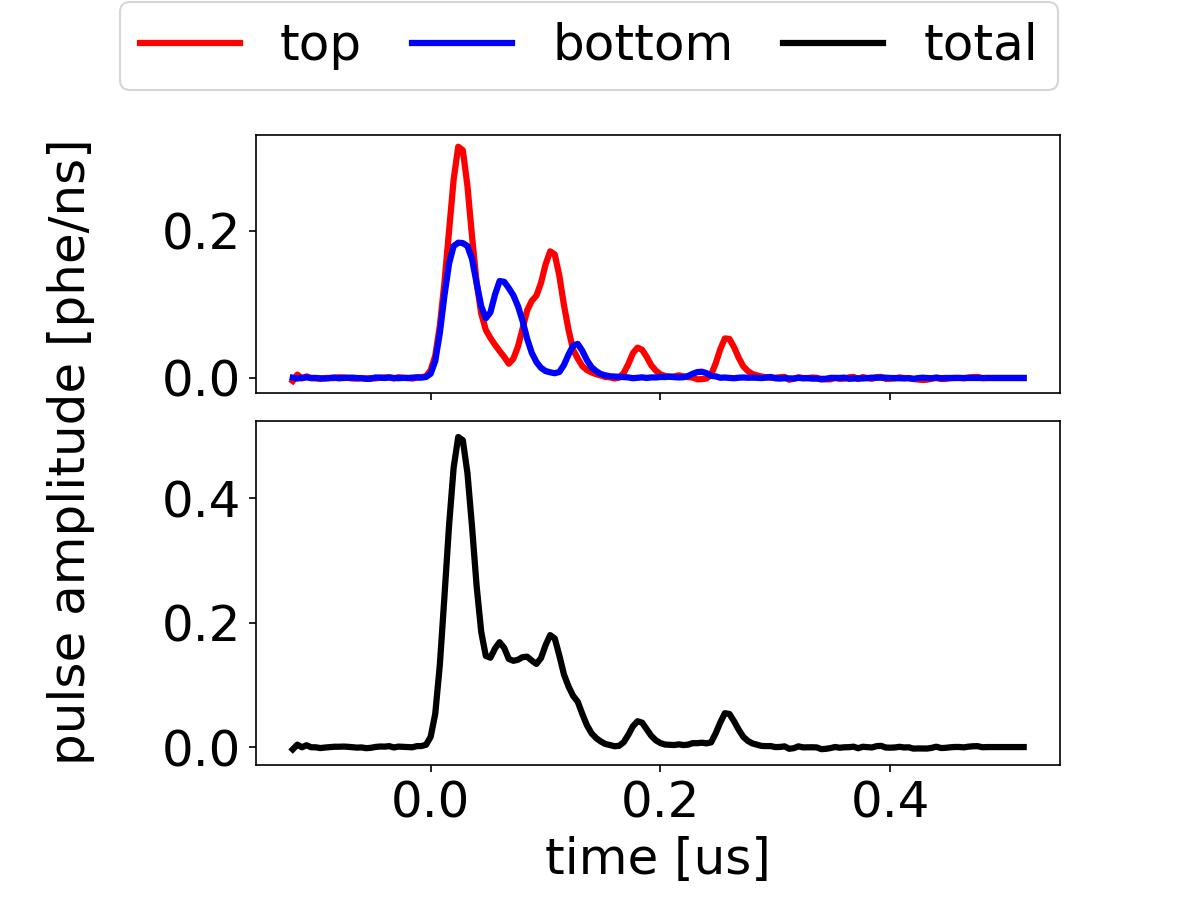
\includegraphics[width=\figurewidth,clip,trim={0 0 0 0}]{Figures/GasTest/exampleWaveforms/proc64767AnodeCone1P1.jpg}
		\caption{}
		\label{fig:anode cone d}
	\end{subfigure}
	\par\bigskip
	\begin{subfigure}[b]{0.7\textwidth}
		\centering
		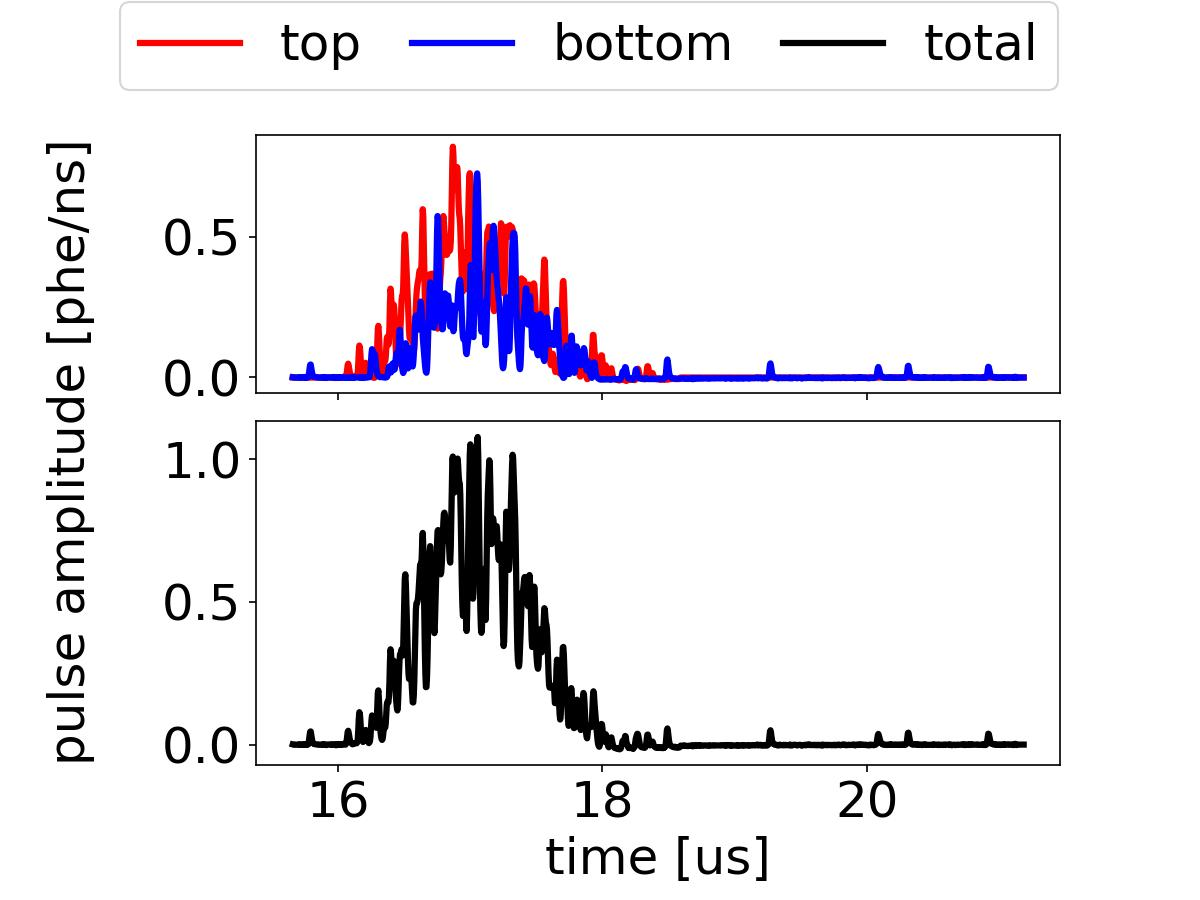
\includegraphics[width=\figurewidth,clip,trim={0 0 0 0}]{Figures/GasTest/exampleWaveforms/proc64767AnodeCone1P2.jpg}
		\caption{}
		\label{fig:anode cone e}
	\end{subfigure}
	\caption[\gtest\ signal: anode cone event (cont.).]{\gtest\ signal: anode cone event (cont.). (c) An example waveform of an anode cone event, zoomed in the range of \SIrange{0}{0.5}{\us}, which shows the primary scintillation light (cartoon part A). (d) An example waveform of an anode cone event, zoomed in the range of \SIrange{15}{21}{\us}, which shows the EL light produced around the anodic grid wires (cartoon part B). }
	\label{fig:anode cone cont}
\end{figure}

%This background from the secondary photon signals in anode cone events has a different pulse shape from \ees . 

%Thus, this cut is performed.  
\paragraph{Cathodic cone event}
\label{sec:events particle cathode cone}
Cathode cone events are the particle radiation events which have energy deposition location in the PTFE reflector cone close to the cathodic grid side (cathode cone). A cartoon of the physical process and an example waveform of cathode cone event are shown in Fig.~\ref{fig:cathode cone}. Similar to anode cone events, this process produce scintillation photons. However, the ionization electrons produced drift to cathode PMT. Therefore, EL light typically is produced during along their trajectories because the electric field in such region is much lower than the EL threshold. The primary scintillation signal normally has a TBA heavier in the cathode side PMT than the anode side PMT, indicating this photon signal is produced in the cathode cone (bottom cone in this case), as expected.

\begin{figure}[!htbp]
	\centering
	\begin{subfigure}[b]{0.8\textwidth}
		\centering
		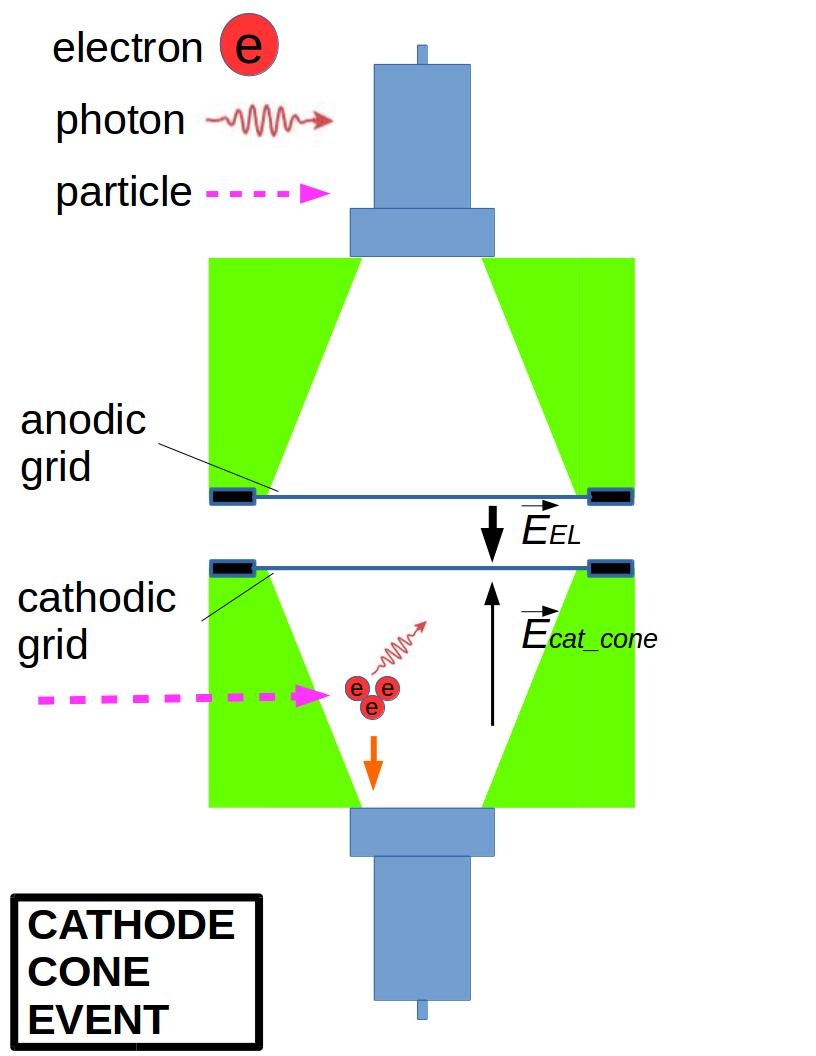
\includegraphics[width=\halfwidth,clip,trim={0 0 0 0},angle=0,origin=c]{Figures/GasTest/WeiDrawEvent/BelowCat.jpg}
		\caption{}
		\label{fig:}
	\end{subfigure}
	\par\bigskip
	\begin{subfigure}[b]{0.7\textwidth}
		\centering
		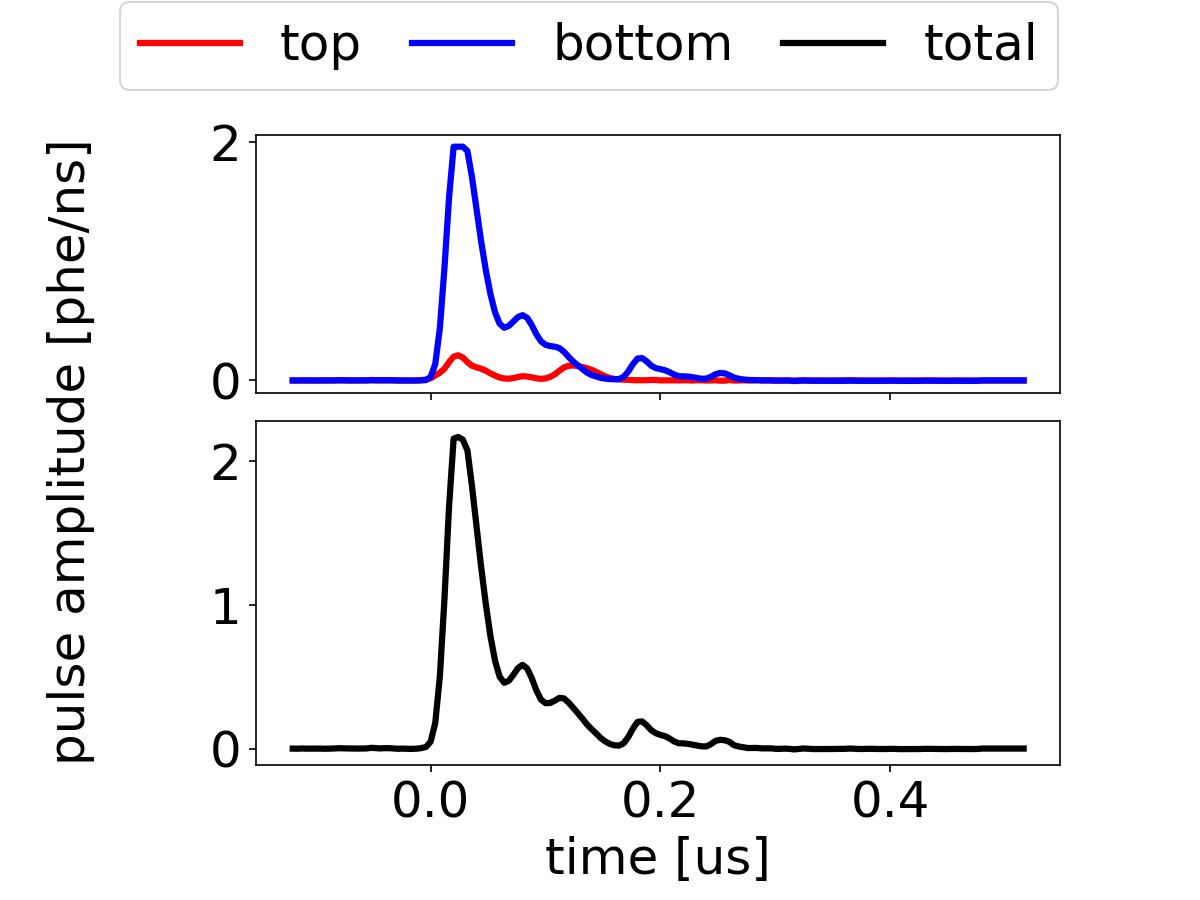
\includegraphics[width=\figurewidth,clip,trim={0 0 0 0}]{Figures/GasTest/exampleWaveforms/proc64767id00000021.jpg}%{Figures/GasTest/CutsValid/wave/testproc65831coinid0.jpg}
		\caption{}
		\label{fig:}
	\end{subfigure}
	\caption[\gtest\ signal: cathode cone event.]{\gtest\ signal: cathode cone event. (a) Cartoon of the process. Primary scintillation light ionization electrons are produced from the particle interaction, and the ionization electrons drift toward the bottom PMT. EL light is typically not produced along the trajectories of the electrons because the electric field in such region is lower than the EL threshold. (b) An example waveform of a cathode cone event. Data were taken at \ddtt{2017}{12}{08}{14}{02}, with \opvtvb\ at \SIlist{+6;-6}{kV}, \opgd\ at \standarddensity .%Data were taken at \ddtt{2018}{03}{12}{11}{41} , with \opvtvb\ at \SI{0}{\kV}, \opgd\ at vacuum.
		% proc13001, procid:101001, Aude rename the dataset name, really confusing now.	
	}
	\label{fig:cathode cone}
\end{figure}

\paragraph[]{S1 S2 event in the cathode corner}
\label{sec:events particle cathode corner}
S1 S2 events in the cathode corner (cathode corner events) are the particle radiation events which have energy deposition location either outside EL region and very close to the cathodic grid or in the corner between the cathodic grid and the cathodic cone. A cartoon of the physical process and an example waveform of cathode corner event are shown in Fig.~\ref{fig:cathode corner}. Similar to anode cone events, this process produce scintillation photons, which is shown in Fig.~\ref{fig:cathode corner b} (left) and the waveform of which is shown in the first \SI{0.3}{\us} in Fig.~\ref{fig:cathode corner c}. Since the free electrons produced in this event is really close to the cathode grid, according to electrostatic study using COMSOL software described in Ref.~\cite{COMSOL2018}, these electrons drift to cathodic grid, pass it, then drift in the EL region, the process of which produces EL photons along the trajectories of the electrons, and finally land on the anodic grid. This EL light production process is illustrated in Fig. ~\ref{fig:cathode corner b} (right), which corresponds to the waveform after \SI{0.5}{\us} in Fig.~\ref{fig:cathode corner c}. The static electric field from COMSOL solution is shown in Fig.~\ref{fig:gtest Comsol cathode corner}. Both the primary scintillation signal  and the secondary EL signal has a balanced TBA, indicating these photon signals are produced either in or really close to the EL region. 

\begin{figure}[!htbp]
	\centering
	\begin{subfigure}[b]{0.8\textwidth}
		\centering
		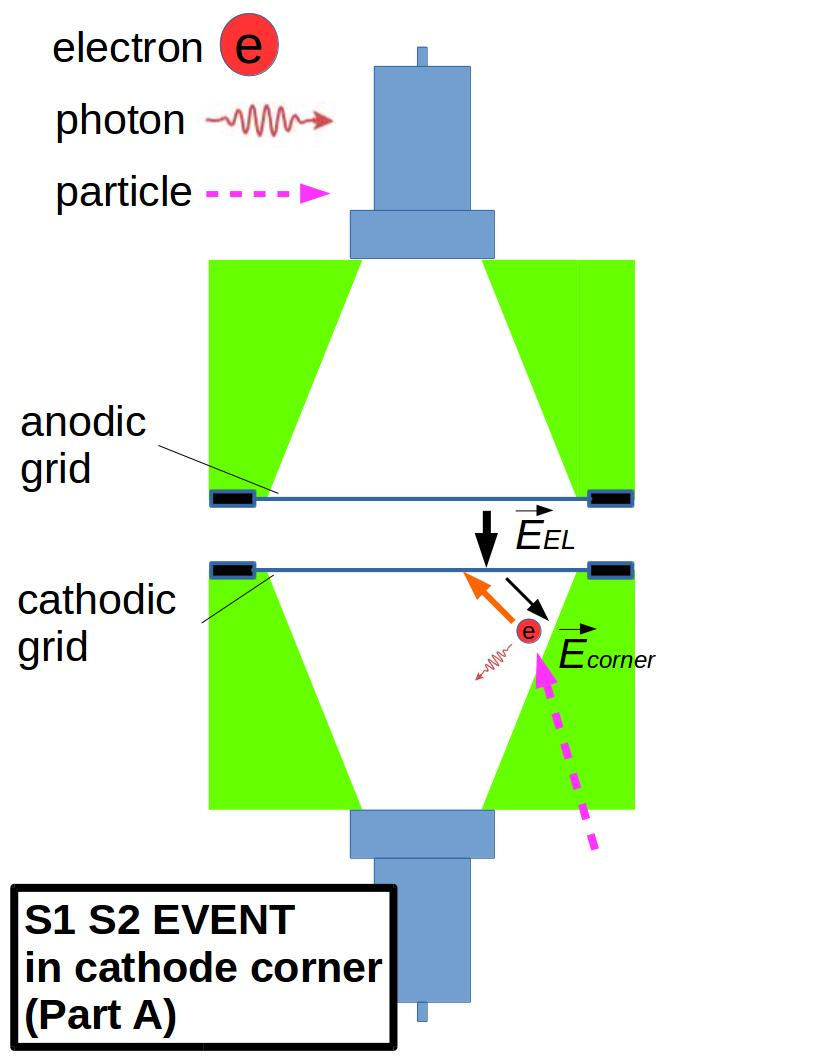
\includegraphics[width=\halfwidth,clip,trim={0 0 0 0},angle=0,origin=c]{Figures/GasTest/WeiDrawEvent/S1S2A.jpg}
%		\caption{}
%		\label{fig:cathode corner a}
%	\end{subfigure}
%	\begin{subfigure}[b]{\halfwidth}
%		\centering
		\includegraphics[width=\halfwidth,clip,trim={0 0 0 0},angle=0,origin=c]{Figures/GasTest/WeiDrawEvent/S1S2B.jpg}
		\caption{}
		\label{fig:cathode corner b}
	\end{subfigure}
	\par\bigskip
	\begin{subfigure}[b]{0.7\textwidth}
		\centering
		\includegraphics[width=\figurewidth,clip,trim={0 0 0 0}]{Figures/GasTest/exampleWaveforms/proc64767id00000145.jpg}%{Figures/GasTest/CutsValid/wave/testproc65831coinid0.jpg}
		\caption{}
		\label{fig:cathode corner c}
	\end{subfigure}
	\caption[\gtest\ signal: S1 S2 event in the cathode corner.]{\gtest\ signal: S1 S2 event in the cathode corner. (a) Cartoon of the process. Left: Primary scintillation light and ionization electrons are produced from the particle interaction, and the ionization electrons drift to the cathodic grid (part A). Right: EL light is produced in the EL region during electrons drifting to the anodic grid (part B). (b) An example waveform of an S1 S2 event in the cathode corner. Data were taken at \ddtt{2017}{12}{08}{14}{02}, with \opvtvb\ at \SIlist{+6;-6}{kV}, \opgd\ at \standarddensity .%Data were taken at \ddtt{2018}{03}{12}{11}{41} , with \opvtvb\ at \SI{0}{\kV}, \opgd\ at vacuum.
		% proc13001, procid:101001, Aude rename the dataset name, really confusing now.	
	}
	\label{fig:cathode corner}
\end{figure}

\begin{figure}[!htbp]
	\centering
	\includegraphics[width=0.8\textwidth,clip,trim={0 0 0 0},angle=0,origin=c]{Figures/GasTest/Comsol/ComsolCathodeCorner.jpg}
	\caption[Electrostatic solution of the \gtest\ detector (grid ring region).]{Electrostatic solution of the \gtest\ detector (grid ring region). This result is solved with \opvtvb\ at \SIlist{+6;-6}{kV} using COMSOL. The white metal structures in the middle of the figure are the cross sections of the grid rings. The contours show the electric potential; the color scales show the norm of electric field; the blue arrows shows the directions of the initial electron drift; the red lines shows the trajectory of electrons that start drifting at \SI{2}{\mm} below the bottom grid: electrons starting at r \SI{<60}{\mm} drift downward, when electrons starting at r \SI{>60}{\mm} drift into the EL region (cathode corner event).}
	\label{fig:gtest Comsol cathode corner}
\end{figure}

\paragraph{S1 S2 event in the EL region}
\label{sec:events particle EL region}
\label{sec:EL region event}
S1 S2 events in the EL region (EL region events) are the particle radiation events which have energy deposition location either in EL region. The process and an example waveforms is shown in Fig.~\ref{fig:EL rad event}. Since the electrons are produced in the energy deposition location in the EL region, these electrons drift in the EL region toward the anodic grid, producing EL photons. The duration of these signals are shorter compared to the \ees s because of the shorter drift length. The total quantity of photon production in this type of events is usually higher than that of an \eee , an anode cone event, and a cathode cone event, because of the free drifted electrons inside the EL region.

\begin{figure}[!htbp]
	\centering
		\begin{subfigure}[b]{.8\textwidth}
		\centering
		\includegraphics[width=\halfwidth,clip,trim={0 0 0 0},angle=0,origin=c]{Figures/GasTest/WeiDrawEvent/S1S2ELRegion.jpg}
		\caption{}
		\label{fig:EL rad event b}
	\end{subfigure}
	\par\bigskip
		\begin{subfigure}[b]{0.7\textwidth}
		\centering
		\includegraphics[width=\figurewidth,clip,trim={0 0 0 0}]{Figures/GasTest/exampleWaveforms/proc64767id00000777.jpg}
		\caption{}
		\label{fig:EL rad event a}
	\end{subfigure}
\begin{comment}
    \par\bigskip
	\begin{subfigure}[b]{0.8\textwidth}
		\centering
		\includegraphics[width=\figurewidth,clip,trim={0 0 0 0}]{Figures/GasTest/exampleWaveforms/proc64767id00000218.jpg}%{Figures/GasTest/CutsValid/wave/testproc65831coinid0.jpg}
		\caption{}
		\label{fig:EL rad event b}
	\end{subfigure}
	\end{comment}
	\caption[\gtest\ signal: S1 S2 event in the EL region.]{\gtest\ signal: S1 S2 event in the EL region. (a) Cartoon of the process. Primary scintillation light and ionization electrons are produced from the particle interaction. The primary scintillation light and the EL light start to be produced simultaneously. (b) An example waveform of an S1 S2 event in the EL region. The primary scintillation light lies on top of the EL light. %(b) another example waveform. 
		Data were taken at \ddtt{2017}{12}{08}{14}{02}, with \opvtvb\ at \SIlist{+6;-6}{kV}, \opgd\ at \standarddensity .%Data were taken at \ddtt{2018}{03}{12}{11}{41} , with \opvtvb\ at \SI{0}{\kV}, \opgd\ at vacuum.
		% proc13001, procid:101001, Aude rename the dataset name, really confusing now.	
	}
	\label{fig:EL rad event}
\end{figure}

\paragraph{High photon count events}
High photon count events are those particle radiation events that are extremely high on energy, therefore producing plenty primary scintillation photon, free drifted electrons, and EL photons during the events. The photon production rate is so high that it exceeds the digitizing ability of the DAQ system (also called saturate the DAQ), causing distortion on waveform recording thus resulting in difficulty of signal classification. These signals may have various origins. Some of these signals have comparable or shorter duration than \ees s, two example waveforms are shown in Fig.~\ref{fig:grid wire rad} and Fig.~\ref{fig:ring rad}. These events might be related to the EL region events, described in Section~\ref{sec:EL region event}, or grid wire radiation and ring radiation, which are the particle radiation events originated from radioactive elements in grid wire and ring materials. 

%\todo{I am not confident about grid ring/wire events.}

The radioactive elements in the ring material can be both from the impurities in the material, e.g. \ce{^{238}U}, \ce{^{232}Th}, and \ce{^{235}U} and from the absorption of air on the material surfaces, e.g. \ce{^{222}Rn}. Among these sources, air radon absorption draw the most concern because of its abundance. The decay activity of radon induced radiation plating per unit of surface area per unit of time ($RA_{\text{\ce{Rn}-rad}}$) is estimated as, 
\begin{align}
	RA_{\text{\ce{Rn}-rad}} = RV_{\text{\ce{Rn}}} h_{\text{eff}} T_{\text{exposure}} \frac{1}{\tau_{\text{eff}}}
\end{align}
where $RV_{\text{\ce{Rn}}}$ is the radon decay activity in the air per unit of volume per unit of time; $h_{\text{eff}}$ is the effective height of radiation plating, in which the radon decay daughter nuclei will plate on material surface; $T_{\text{exposure}}$ is the exposure time of plating; and $\tau_{\text{eff}}$ is the effect decay time constant of radon decay daughter nuclei.
With regard to $RV_{\text{\ce{Rn}}}$ \SI{~48}{\becquerel\per\meter\cubed}, from Ref.~\cite{USEnvironmentalProtectionAgency2017}, $h_{\text{eff}}$ \SI{\sim 1}{\meter},  $\tau_{\text{eff}}$ \SI{\sim 32}{\yr}, from the decay time constant of \ce{^{210}Pb}, the typical daughter nucleus from the radon decay, in Ref.~\cite{Dulieu2008}, and $T_{\text{exposure}}$ \SI{1}{\day}, $RA_{\text{\ce{Rn}-rad}}$ is \SI{\sim 4e-3}{\becquerel\per\meter\squared}. For a \SI{\sim 40}{\cm\squared} grid wire and grid ring total surface area, The total decay activity of radon induced radiation from the ring surface is \SI{\sim e-5}{\becquerel}. These event rates should be relatively rare compared to other processes. %14 Bq total on the ring
%Dulieu2008 is LNE-CEA/LNHB reference
\begin{figure}[!htbp]
	\centering
	\begin{subfigure}[b]{.8\textwidth}
		\centering
		\includegraphics[width=\halfwidth,clip,trim={0 0 0 0},angle=0,origin=c]{Figures/GasTest/WeiDrawEvent/WirePhoto.jpg}
		\caption{}
		\label{fig:}
	\end{subfigure}
	\par\bigskip
	\begin{subfigure}[b]{0.7\textwidth}
		\centering
		\includegraphics[width=\figurewidth,clip,trim={0 0 0 0}]{Figures/GasTest/exampleWaveforms/proc64767id00000117.jpg}%{Figures/GasTest/CutsValid/wave/testproc65831coinid0.jpg}
		\caption{}
		\label{fig:}
	\end{subfigure}
	\caption[\gtest\ signal: grid wire region event.]{\gtest\ signal: grid wire region event. (a) Cartoon of the process. (b) An example waveform. This might be an S1 S2 event in the EL region between the grid wires, when the primary scintillation light is clipped off because the signal amplitude exceeds DAQ dynamic range (PMT saturation). Data were taken at \ddtt{2017}{12}{08}{14}{02}, with \opvtvb\ at \SIlist{+6;-6}{kV}, \opgd\ at \standarddensity .%Data were taken at \ddtt{2018}{03}{12}{11}{41} , with \opvtvb\ at \SI{0}{\kV}, \opgd\ at vacuum.
		% proc13001, procid:101001, Aude rename the dataset name, really confusing now.	
	}
	\label{fig:grid wire rad}
\end{figure}
\begin{comment}
\end{comment}

\begin{figure}[!htbp]
	\centering
	\begin{subfigure}[b]{.8\textwidth}
		\centering
		\includegraphics[width=\halfwidth,clip,trim={0 0 0 0},angle=0,origin=c]{Figures/GasTest/WeiDrawEvent/RingPhoto.jpg}
		\caption{}
		\label{fig:}
	\end{subfigure}
	\par\bigskip
	\begin{subfigure}[b]{0.7\textwidth}
		\centering
		\includegraphics[width=\figurewidth,clip,trim={0 0 0 0}]{Figures/GasTest/exampleWaveforms/proc64767id00000181.jpg}
		\caption{}
		\label{fig:}
	\end{subfigure}
	\caption[\gtest\ signal: grid ring region event.]{\gtest\ signal: grid ring region event. (a) Cartoon of the process. (b) An example waveform. This might be an S1 S2 event in the EL region between the grid rings, when the primary scintillation light is not visible because the light collection efficiency is poor in this region. Data were taken at \ddtt{2017}{12}{08}{14}{02}, with \opvtvb\ at \SIlist{+6;-6}{kV}, \opgd\ at \standarddensity .%Data were taken at \ddtt{2018}{03}{12}{11}{41} , with \opvtvb\ at \SI{0}{\kV}, \opgd\ at vacuum.
		% proc13001, procid:101001, Aude rename the dataset name, really confusing now.	
	}
	\label{fig:ring rad}

\end{figure}
	\begin{comment}
\end{comment}

\paragraph{Multiple scattering events}
\label{sec:events particle multiple scatter}
Multiple scattering events are those with more than one energy deposition location. The common source of these events are a high energy gamma radiation, since it can travel far distance in the detector. The multiple scattering events usually are combinations of the previous mentioned type of events. Two example waveform are shown in Fig.~\ref{fig:multi scatter}: the first one is a multiple scattering event in the anode cone region; the second one is a multiple scattering event in the anode cone region and the EL region.

\begin{figure}[!htbp]
	\centering
	\begin{subfigure}[b]{0.7\textwidth}
		\centering
		\includegraphics[width=\figurewidth,clip,trim={0 0 0 0}]{Figures/GasTest/exampleWaveforms/proc64767id00000054.jpg}
		\caption{}
		\label{fig:}
	\end{subfigure}
\par\bigskip
	\begin{subfigure}[b]{0.7\textwidth}
	\centering
	\includegraphics[width=\figurewidth,clip,trim={0 0 0 0}]{Figures/GasTest/exampleWaveforms/proc64767id00000083.jpg}
	\caption{}
	\label{fig:}
\end{subfigure}
	\caption[\gtest\ signal: multiple scattering event.]{\gtest\ signal: multiple scattering event. (a) An example waveform of a multiple scattering event in the anode cone region. (b) An example waveform of a multiple scattering event in the anode cone region and the EL region. Data were taken at \ddtt{2017}{12}{08}{14}{02}, with \opvtvb\ at \SIlist{+6;-6}{kV}, \opgd\ at \standarddensity .%Data were taken at \ddtt{2018}{03}{12}{11}{41} , with \opvtvb\ at \SI{0}{\kV}, \opgd\ at vacuum.
		% proc13001, procid:101001, Aude rename the dataset name, really confusing now.	
	}
	\label{fig:multi scatter}
\end{figure}

\subsection{Cosmic ray}
\label{sec:events muon}
Cosmic rays, originating outside Earth, are capable of producing showers of secondary particles that reach the \gtest\ detector and giving rise to signals in the detector. Among all secondary particles that raise signals, muons are the most common one because of their abundance and high penetration length in earth atmosphere. Unlike alpha, beta, and gamma particle radiation, a cosmic ray muon has a longer ionization trajectory which travels crossing the whole detector. 
%These cosmic ray muons are normally with high energy that enable them traveling in a straight line in the gas detector in less than \SI{10}{\ns}. 

The long ionization trajectory leads to a large quantity of primary scintillation light and free electron production, which results in a large light production. The minimum stop power of muon is \SI{1.255}{\MeV\per\g\cm\squared} in xenon, from Ref.~\cite{Groom2001}. In xenon gas, the reported average energy to produce a primary scintillation photon ($W_\text{sci}$) and electron-ion pair ($W_\text{ion}$) are \SI{\sim 100}{\eV} 
	\footnote{$W_\text{sci}$ is \SI[separate-uncertainty=false]{111 \pm 16}{\eV} in Ref.~\cite{Carmo2008}, and \SI[separate-uncertainty=false]{72 \pm 6}{\eV} in Ref.~\cite{Fernandes2010}.} 
	and \SI{22}{\eV} 
	\footnote{$W_\text{ion}$ is \SI{22}{\eV} in Ref.~\cite{Fano1963, Ahlen1980, Alvarez2013}.}
	, respectively. Therefore, with detector \opgd\ at \standarddensity , a muon event produce \num{\sim 2e2} primary scintillation photons and \num{\sim e3} per centimeter length of muon trajectory. The large quantity of primary scintillation light and EL light production associated with free electrons results in large signal area detected for a muon event.

Therefore, a cosmic ray muon signal has a different appearance compared to other signals because of its long ionization trajectory and large quantity of primary scintillation light and electron-ion pair production. The appearance of muon signals also varies according to their different trajectories in the detector, which will be discussed below.
%The muon events will be discussed according to their different trajectories in the detector. 
 
\paragraph{EL region muon event}
\label{sec:events muon EL region}
EL region muon events are those events that crosses the EL region, as well as the anode cone region and the cathode cone region. A cartoon and an example waveform are shown in Fig.~\ref{fig:muon EL}. Like particle radiation events, at the very beginning of the signal, primary scintillation photons are produce in the first \SI{500}{\ns}. Simultaneously, during the first \SI{2.5}{\us}, the shown signal is dominated by EL photons, which decrease in time because the electrons in the EL region land on the anodic grid thus stopping EL photon production, illustrated in Fig.~\ref{fig:muon EL b} (left). 
Since free electrons are generated all the way including the EL region, there is prompt EL light that masks the primary scintillation, causing difficulty to distinguish light from these two processes.
At a higher absolute value of \opdv , there is higher photon production per drifted electron, which results in an increase in the signal amplitude and signal area. This high signal amplitude can exceed the dynamic digitization range of the DAQ and results in a clip on the waveform, like in Fig.~\ref{fig:muon EL c}. After all electrons in the EL region reach the anodic grid, the signal is dominated by electrons originally produced in the anode cone drift to the anodic grid and EL photons are produced in the high electric field around the anodic grid, illustrated in Fig.~\ref{fig:muon EL b} (right), which is ``long tail" part of the signal in the range of \SIrange{2.5}{10}{\us} in Fig.~\ref{fig:muon EL c}.

\begin{figure}[!htbp]
	\centering
	\begin{subfigure}[b]{.8\textwidth}
		\centering
		\includegraphics[width=\halfwidth,clip,trim={0 0 0 0},angle=0,origin=c]{Figures/GasTest/WeiDrawEvent/MuonEventA.jpg}
%		\caption{}
%		\label{fig:muon EL a}
%	\end{subfigure}
%	\begin{subfigure}[b]{\halfwidth}
%		\centering
		\includegraphics[width=\halfwidth,clip,trim={0 0 0 0}]{Figures/GasTest/WeiDrawEvent/MuonEventB.jpg}
		\caption{}
		\label{fig:muon EL b}
	\end{subfigure}
	\par\bigskip
	\begin{subfigure}[b]{0.6\textwidth}
		\centering
		\includegraphics[width=\figurewidth,clip,trim={0 0 0 0}]{Figures/GasTest/exampleWaveforms/proc64767id00000107.jpg}
		\caption{}
		\label{fig:muon EL c}
	\end{subfigure}
\caption[\gtest\ signal: EL region muon event.]{\gtest\ signal: EL region muon event. (a) Cartoon of the process. Left: Primary scintillation light and ionization electrons are produced along the muon trajectory, and ionization electrons drift according to the direction of the electric field. EL light also start to be produced by the ionization electrons in the EL region (part A). Right: EL light is produced in the high electric field region around the anodic grid wires (part B). (b) An example waveform of an EL region muon event. The right-angled triangle shape waveform before \SI{2.5}{\us} is the EL light produced in the EL region (cartoon part A). The primary scintillation light is clipped off because of the PMT saturation. The ``long tail" after \SI{2.5}{\us} is the EL light produced around the anodic grid wires (cartoon part B). Data were taken at \ddtt{2017}{12}{08}{14}{02}, with \opvtvb\ at \SIlist{+6;-6}{kV}, \opgd\ at \standarddensity .} 
	\label{fig:muon EL}
\end{figure}

EL region muon events between grid rings are those events that crosses the EL region between the grid rings, without crossing the anode cone region. The cartoon of this process is shown in Fig.~\ref{fig:muon ring a}. Similar to other EL region muon events, these events produces primary scintillation light and EL light between the grid rings. However, since the muon trajectory does not cross the anode cone region, there are no free electrons produced in such region, which leads to the absence of the ``long tail" in the signal, as shown in Fig.~\ref{fig:muon ring b}.  

\begin{figure}[!htbp]
	\centering
	\begin{subfigure}[b]{.8\textwidth}
		\centering
		\includegraphics[width=\halfwidth,clip,trim={0 0 0 0},angle=0,origin=c]{Figures/GasTest/WeiDrawEvent/MuonEventRing.jpg}
		\caption{}
		\label{fig:muon ring a}
	\end{subfigure}
	\par\bigskip
	\begin{subfigure}[b]{0.7\textwidth}
		\centering
		\includegraphics[width=\figurewidth,clip,trim={0 0 0 0}]{Figures/GasTest/exampleWaveforms/proc64767id00000003.jpg}%{Figures/GasTest/CutsValid/wave/testproc65831coinid0.jpg}
		\caption{}
		\label{fig:muon ring b}
	\end{subfigure}
	\caption[\gtest\ signal: muon event between the grid rings.]{\gtest\ signal: muon event between the grid rings. (a) Cartoon of the process. This process is similar to that of the EL region muon event except there are no electrons produced in the anode cone region. (b) An example waveform. The absence of ``long tail"  is because of the absence of electrons produced in the anode cone region. Data were taken at \ddtt{2017}{12}{08}{14}{02}, with \opvtvb\ at \SIlist{+6;-6}{kV}, \opgd\ at \standarddensity .%Data were taken at \ddtt{2018}{03}{12}{11}{41} , with \opvtvb\ at \SI{0}{\kV}, \opgd\ at vacuum.
		% proc13001, procid:101001, Aude rename the dataset name, really confusing now.	
	}
	\label{fig:muon ring}
\end{figure}

\paragraph{Anode cone muon event}
\label{sec:events muon anode cone}
Anode cone muon events are those events that crosses only the anode cone region. A cartoon and an example waveform are shown in Fig.~\ref{fig:muon anode}. At the very beginning of the signal, primary scintillation photons are produce in the first \SI{500}{\ns}, the process and waveform of which are shown in Fig.~\ref{fig:muon anode a} and Fig.~\ref{fig:muon anode d}. Next, electrons originally produced in the anode cone drift to the anodic grid and EL photons are produced in the high electric field around the anodic grid, the process and waveform of which are shown in Fig.~\ref{fig:muon anode b} and Fig.~\ref{fig:muon anode e}. 

\begin{figure}[!htbp]
	\centering
	\begin{subfigure}[b]{0.8\textwidth}
		\centering
		\includegraphics[width=\halfwidth,clip,trim={0 0 0 0},angle=0,origin=c]{Figures/GasTest/WeiDrawEvent/AnodeMuonEventA.jpg}
%		\caption{}
%		\label{fig:muon anode a}
%	\end{subfigure}
%	\begin{subfigure}[b]{\halfwidth}
%		\centering
		\includegraphics[width=\halfwidth,clip,trim={0 0 0 0}]{Figures/GasTest/WeiDrawEvent/AnodeMuonEventB.jpg}
		\caption{}
		\label{fig:muon anode b}
	\end{subfigure}
	\par\bigskip
	\begin{subfigure}[b]{0.7\textwidth}
		\centering
		\includegraphics[width=\figurewidth,clip,trim={0 0 0 0}]{Figures/GasTest/exampleWaveforms/proc64767AnodeMuon1.jpg}
		\caption{}
		\label{fig:muon anode c}
	\end{subfigure}
	\caption[\gtest\ signal: anode cone muon event.]{\gtest\ signal: anode cone muon event. (a) Cartoon of the process. This process is similar to that of the EL region muon event except for there are no electrons produced in the EL region. (b) An example waveform of an anode muon cone event. The absence of the ``right-angled triangle shape waveform"  is because of the absence of electrons produced in the EL region. Data were taken at \ddtt{2017}{12}{08}{14}{02}, with \opvtvb\ at \SIlist{+6;-6}{kV}, \opgd\ at \standarddensity .}
	\label{fig:muon anode}
\end{figure}
\begin{figure}[!htbp]\ContinuedFloat
	\centering
	\begin{subfigure}[b]{0.7\textwidth}
		\centering
		\includegraphics[width=\figurewidth,clip,trim={0 0 0 0}]{Figures/GasTest/exampleWaveforms/proc64767AnodeMuon1P1.jpg}
		\caption{}
		\label{fig:muon anode d}
	\end{subfigure}
		\par\bigskip
\begin{subfigure}[b]{0.7\textwidth}
	\centering
	\includegraphics[width=\figurewidth,clip,trim={0 0 0 0}]{Figures/GasTest/exampleWaveforms/proc64767AnodeMuon1P2.jpg}
	\caption{}
	\label{fig:muon anode e}
\end{subfigure}
	\caption[\gtest\ signal: anode cone muon event (cont.).]{\gtest\ signal: anode muon cone event (cont.). (c) An example waveform of an anode muon cone event, zoomed in the range of \SIrange{0}{5}{\us}, which shows the primary scintillation light (cartoon part A). (d) An example waveform of an anode cone muon event, zoomed in the range of \SIrange{6}{50}{\us}, which shows the EL light produced around the anodic grid wires (cartoon part B).}
	\label{fig:anode muon cont}
\end{figure}

\paragraph{Cathode cone muon event}
\label{sec:events muon cathode cone}
Cathode cone muon events are those events that crosses only the cathode cone region. A cartoon and an example waveform are shown in Fig.~\ref{fig:cathode muon}. At the very beginning of the signal, primary scintillation photons are produce in the first \SI{500}{\ns}, the process and waveform of which are shown in Fig.~\ref{fig:cathode muon a} and Fig.~\ref{fig:cathode muon b}. Next, electrons originally produced in the cathode cone drift to the cathode PMT associated with few EL photons production in this low electric field cathode cone region. 

\begin{figure}[!htbp]
	\centering
		\begin{subfigure}[b]{.8\textwidth}
		\centering
		\includegraphics[width=\halfwidth,clip,trim={0 0 0 0},angle=0,origin=c]{Figures/GasTest/WeiDrawEvent/CathodeMuonEvent.jpg}
		\caption{}
		\label{fig:cathode muon a}
	\end{subfigure}
\par\bigskip
	\begin{subfigure}[b]{0.7\textwidth}
		\centering
		\includegraphics[width=\figurewidth,clip,trim={0 0 0 0}]{Figures/GasTest/exampleWaveforms/proc64767id00000007.jpg}%{Figures/GasTest/CutsValid/wave/testproc65831coinid0.jpg}
		\caption{}
		\label{fig:cathode muon b}
	\end{subfigure}
	\caption[\gtest\ signal: cathode cone muon event.]{\gtest\ signal: cathode cone muon event. (a) Cartoon of the process. This process is similar to that of the EL region muon event except for there are no electrons produced in the EL region or the anode cone region. (b) An example waveform of a cathode muon cone event. The absence of the ``right-angled triangle shape waveform" and the ``long tail"  is because of the absence of electrons produced in the EL region and the anode cone region.  Data were taken at \ddtt{2017}{12}{08}{14}{02}, with \opvtvb\ at \SIlist{+6;-6}{kV}, \opgd\ at \standarddensity .%Data were taken at \ddtt{2018}{03}{12}{11}{41} , with \opvtvb\ at \SI{0}{\kV}, \opgd\ at vacuum.
		% proc13001, procid:101001, Aude rename the dataset name, really confusing now.	
	}
	\label{fig:cathode muon}
\end{figure}

\subsection{Other miscellaneous sources}
\label{sec:events misc}
\paragraph{Electrical noise} 
\label{sec:events noise}
Electrical noise are the disturbance in an electrical system during signal transfer. Electrical noise can come from both internal and external sources to the system, and can add to the systematic fluctuation of other signals from the \gtest detector. This systematic fluctuation is characterized by the baseline fluctuation, whose amplitude is \SI{\sim 0.36}{\mV}, which is very small compared to signal amplitude of the wanted signals. 

Electrical noise from the external electrical grounding of the infrastructures and the KNF pump, however, has an amplitude up to \SI{5}{\mV} and is capable of start a separate pulse recording sometimes; this type of electrical noise is called electrical noise signals. An example waveform of electrical noise signal is shown in Fig.~\ref{fig:noise}. As shown in this figure, an electrical noise signal is likely to have the waveforms in both PMTs overlapping. %a comparable signal negative maximum amplitude and signal positive amplitude, and a small and sometimes negative signal total pulse area. 
The waveform in each PMT is bipolar and symmetric; that is, the positive and negative maxima of the waveform amplitude are about the same. The bipolar and symmetric aspect of the waveform leads to a near-zero integral of the signal area, which don't give a meaningful waveform shape RQs because these RQ algorithms are designed for a unipolar signal. 
%The negative total pulse area usually also makes it impossible to find the pulse RQs of characteristic waveform percentiles to conduct further signal \ees\ selections. 
Therefore, to reduce the influence of these electrical noise signals, the KNF pump is turn off during all measurements and we improved on the electrical grounding of infrastructure. After this improvement, electrical noise signals occur at a rate of \SI{\sim 2}{\Hz}, which are further addressed by signal selections based on the bipolar feature of the noise signals. 

\begin{figure}[!p]
    \centering
	\begin{subfigure}[b]{0.7\textwidth}
	\centering
	\includegraphics[width=\figurewidth,clip,trim={0 0 0 0}]{Figures/GasTest/exampleWaveforms/proc64767id00000034.jpg}%{Figures/GasTest/CutsValid/wave/testproc65831coinid0.jpg}
	\caption{}
	\label{fig:}
\end{subfigure}
\caption[\gtest\ signal: electronic noise.]{\gtest\ signal: electronic noise signal. (a) An example waveform. Data were taken at \ddtt{2017}{12}{08}{14}{02}, with \opvtvb\ at \SIlist{+6;-6}{kV}, \opgd\ at \standarddensity .%Data were taken at \ddtt{2018}{03}{12}{11}{41} , with \opvtvb\ at \SI{0}{\kV}, \opgd\ at vacuum.
	% proc13001, procid:101001, Aude rename the dataset name, really confusing now.	
}
\label{fig:noise}
\end{figure}

\paragraph{PMT dark current}
\label{sec:events dark current}
PMT dark current usually refers to the signal from the thermal electron emission from the photocathode and dynode surfaces, which are charges generated in the PMT when no photon ejects photoelectrons from the photocathode surface. The thermal electrons from the photocathode surface, like photoelectrons, if landing on the effective area of the first dynode, will be amplified by the PMT and produce a \sphe -like signal. Such \sphe -like signals of the PMT dark current are a major concern, since they are not distinguishable from \sphe s in signals of interest. The thermal electrons from other surfaces may also be amplified by the PMT dynode chain and produce signals that are distinguishably smaller than \sphe , thus drawing less concern. 

A random coinciding of \sphe -like signals (dark current is one of the most common sources of \sphe -like signals) between two PMTs, is called an accidental coinciding signal. The PMTs that are used in this study have a \SI{\sim 1}{\kHz} dark current rate.  This rate leads to a \SI{\sim 3.4}{\Hz} rate of the accidental coinciding signals with regard to CWW of \SI{1.7}{\us}. 
 
 %The \sphe\ source is not limited to dark current. 
\begin{figure}[!p]
	\centering
	\begin{subfigure}[b]{0.7\textwidth}
		\centering
		\includegraphics[width=\figurewidth,clip,trim={0 0 0 0}]{Figures/GasTest/exampleWaveforms/proc64767id00000053.jpg}%{Figures/GasTest/CutsValid/wave/testproc65831coinid0.jpg}
		\caption{}
		\label{fig:}
	\end{subfigure}
	\caption[\gtest\ signal: PMT dark current accidental coinciding.]{\gtest\ signal: PMT dark current accidental coinciding. (a) An example waveform. Data were taken at \ddtt{2017}{12}{08}{14}{02}, with \opvtvb\ at \SIlist{+6;-6}{kV}, \opgd\ at \standarddensity .%Data were taken at \ddtt{2018}{03}{12}{11}{41} , with \opvtvb\ at \SI{0}{\kV}, \opgd\ at vacuum.
		% proc13001, procid:101001, Aude rename the dataset name, really confusing now.	
	}
	\label{fig:pmt dark current}
\end{figure}

\todo{should I talk about PMT afterpulsing?}

\paragraph{PTFE fluorescence}
\label{sec:events PTFE fluo}
PTFE fluorescence is the phenomenon in which PTFE emits photons that it absorbed. This delay emission normally appears in forms of \sphe s following a high quantity of photon production, and increase the \sphe\ rate succeeding. The rate of after emission photons (fluorescence rate) roughly follows an exponential decay model:
\begin{align}
	 \text{fluorescence rate} = f_{\text{FR}}\ A\frac{1}{\tau} \exp \left( -\frac{t}{\tau} \right) 
\end{align} 
where $\tau$ is the decay time constant; t is the time since the previous photon production; A is quantity of photons in the previous photon production that are absorb by the PTFE; and $f_{\text{FR}}$ is the fluorescence ratio, which is the ratio of the number of photons emitted after by the PTFE material to the number of photons absorbed by the PTFE material.

Measurements show that fluorescence rates, decay times $\tau$, and fluorescence ratio $f_{\text{FR}}$ have a various range. This might be caused by different conditions of synthesis, as described in Ref.~\cite{Gachkovskii1969}. This effect is also believed to cause the slow decay of electron signal in liquid xenon TPCs. A decay time of \SI{2.3}{\ms} is reported in Ref.\cite{Sorensen2018}. A decay time of \SI{10}{\ms} is reported in internal review in \luxe .  

To illustrate the large rate of \sphe s that follows a large-area signal, we look at 1-\si{\ms} windows before and after a large photon production. In the succeeding 1-\si{\ms} window after t = \num{0}, which is the time when the selected large signal happened, as shown with the selected large signal in Fig.~\ref{fig:ptfe fluo b}, Fig.~\ref{fig:ptfe fluo c}, we see 33 \sphe s. In comparison, we see only 1 \sphe\ in the earlier 1-\si{\ms} window, as shown in the same figure before t = \num{0}. 
%An example waveform of an event with large photon production and the waveform in its preceding and succeeding window is shown in Fig.~\ref{fig:ptfe fluo b}. A waveform in its preceding window is shown in Fig.~\ref{fig:ptfe fluo b} to compare the \sphe\ rate. In the comparison example, 33 \sphe s in a succeeding window of \SI{\sim 1000}{\us} are recorded, when only 1 \sphe\ are recorded in a preceding window with the same window width. 
This increasing rate of \sphe\ increases the probability of accidental coinciding between two PMT channels, as shown in Fig.~\ref{fig:ptfe fluo d}; given the practical choice of our CCW, this random accidental coinciding, like PMT dark current, is a potential source of background that looks like \ees s.
   \begin{comment}
\begin{subfigure}[b]{0.8\textwidth}
\centering
\includegraphics[width=\figurewidth,clip,trim={0 0 0 0}]{Figures/GasTest/exampleWaveforms/proc64767PTFEFluo1.jpg}
\caption{}
\label{fig:ptfe fluo a}
\end{subfigure}
\par\bigskip
\end{comment}
\begin{figure}[!p]
	\centering
   	\begin{subfigure}[b]{1.0\textwidth}
   	\centering
   	\includegraphics[width=\figurewidth,clip,trim={0 0 0 0}]{Figures/GasTest/exampleWaveforms/proc64767PTFEFluo2x.jpg}
   	\caption{}
   	\label{fig:ptfe fluo b}
   \end{subfigure}
	\caption[\gtest\ signal: PTFE fluorescence after an event with large photon production.]{\gtest\ signal: PTFE fluorescence after an event with large photon production. (a) An example waveform \SI{1000}{\us} before and after a large-area signal. There are more \sphe s after an event with large photon production than before. The \sphe\ rate before this large-area event is representative of the average \sphe\ rate. Data were taken at \ddtt{2017}{12}{08}{14}{02}, with \opvtvb\ at \SIlist{+6;-6}{kV}, \opgd\ at \standarddensity .}
	\label{fig:ptfe fluo}
\end{figure}
\begin{figure}\ContinuedFloat
	\centering
	\begin{subfigure}[b]{0.7\textwidth}
		\centering
		\includegraphics[width=\figurewidth,clip,trim={0 0 0 0}]{Figures/GasTest/exampleWaveforms/proc64767PTFEFluo2P1.jpg}
		\caption{}
		\label{fig:ptfe fluo c}
	\end{subfigure}
	\par\bigskip
	\begin{subfigure}[b]{0.7\textwidth}
		\centering
		\includegraphics[width=\figurewidth,clip,trim={0 0 0 0}]{Figures/GasTest/exampleWaveforms/proc64767PTFEFluo2P2.jpg}
		\caption{}
		\label{fig:ptfe fluo d}
	\end{subfigure}
	\caption[\gtest\ signal: PTFE fluorescence after an event with large photon production (cont.).]{\gtest\ signal: PTFE fluorescence after an event with large photon production (cont.). (b) An example waveform, zoomed in the range of \SIrange{0}{17}{\us}, which shows the signal with large photon production.  (c) An example waveform, zoomed in the range of \SIrange{87}{89}{\us}, which shows PTFE fluorescence induced \sphe s accidental coinciding between the two PMTs. This accidental coinciding signal looks like an \ees .}
	\label{fig:ptfe fluo cont}
\end{figure}

With these examples in mind, we can quantify the fluorescence process by looking at the delayed \sphe\ rate follow large-area signals over different characteristic timescales. The \sphe\ rate of this PTFE fluorescence increase if the ELD has a recent large photon production. Fig.~\ref{fig:PMT PFTE fluo} shows the photon rate after source signals: This photon fluorescence rate increases as the signal area of source signals increases; and this photon fluorescence rate decreases over time. 

\begin{figure}[!p]
	\centering
	\begin{subfigure}[t]{\twofigurewidth}
		\centering
		\includegraphics[width=\textwidth,clip,trim={0 0 0 0},angle=0,origin=c]{Figures/GasTest/DatasetQuality/topPMTPTFEFluoEva64767.jpg}
		\caption{}
		\label{fig:PMT PFTE fluo top}
	\end{subfigure}
	\begin{subfigure}[t]{\twofigurewidth}
		\centering
		\includegraphics[width=\textwidth,clip,trim={0 0 0 0}]{Figures/GasTest/DatasetQuality/botPMTPTFEFluoEva64767.jpg}
		\caption{}
		\label{fig:PMT PFTE fluo bottom}
	\end{subfigure}
	\caption[Photon fluorescence rate after photon production in the ELD.]{Photon fluorescence rate after photon production in the ELD: (a) top PMT; (b) bottom PMT. The solid lines show the medians. The color bands show the \SIrange{25}{75}{\percent} bands. The choice of bin edges is made to get enough statistics in each bin. }
	\label{fig:PMT PFTE fluo}
\end{figure}

An estimation of fluorescence rate, decay time $\tau$, and fluorescence ratio $f_{\text{FR}}$ is carried out by studying the photon rate in the waveform after a signal production of larger than \SI{e4}{\phe} in the range of \SIrange{200}{600}{\us} after the end time of signal. The choice of the smaller value of the succeeding window is to avoid the influence from the anode cone events correlating signals, whereas the choice of the later time of the succeeding window is to avoid the influence the background rate, which is mostly contributed by dark current. In the chosen signal ranges, the background rate is \SI{\sim 1}{\kHz} per PMT, mostly contributed by PMT dark current. This rate is small compared to fluorescence rate (median \SI{\sim 20}{\kHz}) per PMT, thus negligible in this estimation. Therefore,
\begin{align}
	\text{photon rate} & \approx \text{fluorescence rate}\ \big( + \text{background rate (dark current, etc.) \big)} \\
	&\propto \frac{1}{\tau} \exp \left( -\frac{t}{\tau} \right) \label{eqn:fluo}
\end{align} 
To better estimate the photon rate profile and find the decay time $\tau$, we fit this exponential decay profile to binned data in the succeeding window. To combine multiple events to reduce the statistical error, individual events are normalized by their signal areas in the range of \SIrange{0}{1000}{\us} and then co-added by bin; the resulting graph is fitted, and shown in 
%each waveform in the succeeding window is normalized so that the integrated area in the choice of time range is 1. Then, by averaging these normalize waveforms and fitting the average waveform with Eqn.~\ref{eqn:fluo} profile, we get a $\tau$ of \SI{375 \pm 36}{\us}, as shown in 
Fig.\ref{fig:PMT PTFE fluo tau}: $\tau$ of \SI{407 \pm 35}{\us}.

The fluorescence ratio $f_{\text{FR}}$ is defined as,
\begin{align}
f_{\text{FR}} &= \frac{\text{\#\ photons reemitted}}{\text{\#\ photons absorbed}}
\end{align}
which is the ratio of the number of photons that are reemitted from the PTFE after a large-area event to the number of photons that are absorbed by the PTFE in a large-area event. 

The number of photons reemitted is estimated from the exponential decay profile defined above and the number of photons in the succeeding \SIrange{200}{600}{\ns} window after the end of the large-area signal. From the estimated decay time, the ratio of the number of reemitted photons in the succeeding window ($N_{\text{SW}}$) to the total number of reemitted photons is derived, noted as $P_{\text{SW}}$: 

\begin{align}
P_{\text{SW}} \approx& \frac{N_{\text{SW}}}{\text{\#\ photons reemitted}}.
\end{align}

The number of reemitted photons in the succeeding window is estimated from the number of photons reemitted detected in the succeeding window ($A_{\text{SW}}$) and the light collection efficiency for photons starting from PTFE surface:  
\begin{align}
%\text{\#\ photons reemitted} \approx& \frac {
%	\frac{\text{\normalsize \#\ photons in the succeeding window} }
%	{ \text{\normalsize estimated profile ratio of the succeeding window} } 
%	}
%	{\text{\normalsize average light collection efficiency at the location of PTFE}} ,
A_{\text{SW}} \approx& \text{LCE}_{\text{PTFE}} N_{\text{SW}}. 
\end{align}
where $\text{LCE}_{\text{PTFE}}$ is the average light collection efficiency for photons starting from PTFE surface. 
%which is estimated by the same method  described in Section~\ref{sec:gtest light collection}. 

On the other hand, the number of photons absorbed by PTFE is estimated from the total number of photons the source large-area signal ($N_{\text{source}}$) and the light collection simulation of the fraction of photons that PTFE absorbed:
\begin{align}
\text{\#\ photons absorbed} \approx& \text{LCF}_{\text{EL-PTFE}} N_{\text{source}}
\end{align}
where $\text{LCF}_{\text{EL-PTFE}}$ is the average fraction of photons absorbed by PTFE in the simulation with photons starting in the EL region, the location where the source signals happen. 

The total number of photons the source large-area signal ($N_{\text{source}}$) is related to the detected signal area ($A_{\text{source}}$) and light collection efficiency of the source signals in the EL region ($\text{LCE}_{\text{EL}}$).
\begin{align}
%\text{\#\ photons absorbed} \approx& \frac{
%	\frac{\text{\normalsize \#\ photons in the signal}}
%	{\text{\normalsize average light collection efficiency at the location of the EL region}} 
%	}
%	{\text{\normalsize average absorption fraction by PTFE}} .
A_{\text{source}} \approx& \text{LCE}_{\text{EL}}  N_{\text{source}}
\end{align}

Therefore, from the measure ratio of signal area in the succeeding window ($A_{\text{SW}}$) to the source signal area ($A_{\text{source}}$), the result of which is shown in Fig.~\ref{fig:PMT PTFE fluo ratio}, we can derive the fluorescence ratio $f_{\text{FR}}$. 
$P_{\text{SW}}$ is \num{\sim 0.23} with regard to the decay time $\tau$. $\text{LCE}_{\text{PTFE}}$ is \SI{2.85}{\percent} (top PMT: \SI{1.35}{\percent}, bottom PMT: \SI{1.50}{\percent}); $\text{LCE}_{\text{EL}}$ is \SI{1.70}{\percent} (top PMT: \SI{0.85}{\percent}, bottom PMT: \SI{0.85}{\percent}); and $\text{LCF}_{\text{EL-PTFE}}$ is \SI{79.3}{\percent} (top cone: \SI{39.0}{\percent}, bottom cone: \SI{40.3}{\percent}), which are estimated by using the same method as described in Section~\ref{sec:gtest light collection} using PTFE reflectivity of \num{0.4}. With the ratio of $A_{\text{SW}}$ to $A_{\text{source}}$ \num{\sim 0.5e-3}, $f_{\text{FR}}$ is \num{\sim 1.6e-3}. This result has a big uncertainty (up to \num{1e-3}) due to statistic errors, and the systematic errors in the light collection efficiency and the absorption fraction, resulting from the uncertainty in the PTFE reflectivity value. 

\begin{figure}[!p]
		\centering
		\includegraphics[width=.8\textwidth,clip,trim={0 0 0 0},angle=0,origin=c]{Figures/GasTest/DatasetQuality/PMTPTFEFluoTau0200060064767.jpg}
		\caption[The average of scaled waveform in the range of \SIrange{0}{2000}{\us} since source signals.]{The average of scaled waveform in the range of \SIrange{0}{2000}{\us} since source signals. See text for details.}
		\label{fig:PMT PTFE fluo tau}
	\end{figure}

	\begin{figure}[!p]
		\centering
		\includegraphics[width=.8\textwidth,clip,trim={0 0 0 200}]{Figures/GasTest/DatasetQuality/PMTPTFEFluoRatio0200060064767.jpg}
		\caption[The ratio of the number of photon in the range of \SIrange{200}{600}{\us} since source signals to the number of photons in the source signal.]{The ratio of the number of \sphe s in the range of \SIrange{200}{600}{\us} since source signals to the number of \sphe s in the source signal.}
		\label{fig:PMT PTFE fluo ratio}
	\end{figure}


\paragraph{Cherenkov radiation} 
\label{sec:events Cherenkov}
\todo{think about gamma particle induced cherenkov, and whether the calculation is correct.}
Cherenkov radiation is the photon radiation process when a charged particle is traveling through a medium with its speed higher than the speed of light in the medium. The charged particle could be an external charged particle or electrons that originate from energy loss of external particle in the medium. Because of the photon production in Cherenkov radiation process, especially when this process happens in the PTFE materials (and the PMT windows), it is considered to one of the sources of the signals in \gtest . A cartoon for the physical process and an example waveform of extremely narrow pulse are shown in Fig.~\ref{fig:Chrenkov}. %

The quantity of photon production in Cherenkov radiation process is estimated by its theoretical spectrum following Frank–Tamm formula. A simplified approximation for Frank–Tamm formula from Ref.~\cite{Jackson1999} Eqn.~{14.133} shows:
\begin{align}
	\frac{\d I(\omega)}{\d x} = \frac{e^2 \omega}{c^2} \left[ 1-\frac{1}{\beta^2 \epsilon(\omega)} \right] 
	\label{eqn:CherenkovE}
\end{align}
where $\omega$ is the frequency of Cherenkov radiation, I($\omega$) is the energy intensity of frequency $\omega$, $\epsilon$($\omega$) is the relative permittivity of the medium, and $\beta$ is the speed of the charged particle. 
$\omega$ satisfies that $\beta^2 \epsilon$($\omega$) is larger than one, so that the energy intensity is positive.
The number intensity N($\omega$) can be derived from Eqn.~\ref{eqn:CherenkovE}
\begin{align}
	\frac{\d N(\omega)}{\d x} = \frac{\alpha}{c} \left[1-\frac{1}{\beta^2 \epsilon(\omega)} \right] 
	\label{eqn:CherenkovN}
\end{align}
where $\alpha \equiv e^2/\hbar c \approx 1/137$ is the fine structure constant. The total quantities of photons (N) is the integral over frequency and distance of Eqn.~\ref{eqn:CherenkovN}.

%\todo{resolve the 2 pi difference between Jackson and here. 
%	http://large.stanford.edu/courses/2014/ph241/alaeian2/}
% Answer: simple \omega = 2 \pi f

\begin{figure}[!p]
	\centering
	\begin{subfigure}[b]{.4\textwidth}
		\centering
		\includegraphics[width=\figurewidth,clip,trim={0 0 0 0},angle=0,origin=c]{Figures/GasTest/WeiDrawEvent/Cherenkov.jpg}
		\caption{}
		\label{fig:Chrenkov a}
	\end{subfigure}
	\begin{subfigure}[b]{.4\textwidth}
		\centering
		\includegraphics[width=\figurewidth,clip,trim={0 0 0 0},angle=0,origin=c]{Figures/GasTest/WeiDrawEvent/MuonVac.jpg}
		\caption{}
		\label{fig:}
	\end{subfigure}
	\par\bigskip
	\begin{subfigure}[b]{0.6\textwidth}
		\centering
		\includegraphics[width=\figurewidth,clip,trim={0 0 0 0}]{Figures/GasTest/exampleWaveforms/proc64767id00000002.jpg}%{Figures/GasTest/CutsValid/wave/testproc65831coinid0.jpg}
		\caption{}
		\label{fig:Chrenkov b}
	\end{subfigure}
	\caption[\gtest\ signal: Cherenkov radiation in PTFE.]{\gtest\ signal: Cherenkov radiation in PTFE. (a) Cartoon of the process in which Cherenkov radiation is produced in PTFE. The Cherenkov radiation comes from the electrons created in a gamma particle event. (b) Cartoon of the process in which Cherenkov radiation is produced in PTFE after a muon particle crossing the detector. (1) If the detector is in vacuum, even though the muon particle crosses the cone regions, there is no primary scintillation or ionization inside the ELD active volume, and only Cherenkov radiation signals from this muon event in PTFE are observed. (2) A muon particle does not cross the cone regions. Cherenkov radiation signals from this muon in PTFE are observed. (c) An example waveform of a Cherenkov radiation event. Data were taken at \ddtt{2017}{12}{08}{14}{02}, with \opvtvb\ at \SIlist{+6;-6}{kV}, \opgd\ at \standarddensity .%Data were taken at \ddtt{2018}{03}{12}{11}{41} , with \opvtvb\ at \SI{0}{\kV}, \opgd\ at vacuum.
		% proc13001, procid:101001, Aude rename the dataset name, really confusing now.	
	}
	\label{fig:Chrenkov}
\end{figure}

A portion of these Cherenkov radiation photons can be seen by the PMTs, since PTFE is partially transparent to these photons. The duration of Cherenkov radiation event light production is the duration of charged particle energy loss process, which is typically very short (\SIrange{\sim 1}{10}{\ns}). The number of photons ($A_{\text{Che}}$) detected by the PMTs for a typical \SI{1}{\MeV} electron is estimated using the following parameters:  
\begin{align}
	A_{\text{Che}} \approx N_{\text{Che}} f_{\text{to-surface}} \exp \left ( - d_{\text{to-surface}}/d_{\text{atten}} \right ) \text{LCE}_{\text{PTFE}} 
\end{align}
where $N_{\text{Che}}$ is the number of produced Cherenkov radiation photons which the PMTs are sensitive to; $f_{\text{to-surface}}$ is the fraction of Cherenkov radiation photons going toward the PTFE surface; $d_{\text{to-surface}}$ is the distance from the location of Cherenkov radiation produce to the PTFE surface; $d_{\text{atten}}$ is the attenuation length of PMT sensitive Cherenkov radiation photons; and $\text{LCE}_{\text{PTFE}}$ is the light collection efficiency for photons exiting PTFE surfaces. 

$N_{\text{Che}}$ is related to PMT sensitivity, we take the PMT sensitive photon wavelength in the range of \SIrange{160}{650}{\nm} (the spectral response range for PMT R11410-10, as described in Ref.~\cite{HamamatsuPhotonics2006}). $N_{\text{Che}}$ is also related the PTFE refractive index, and electron stopping distance, which are approximately 2 ($\epsilon$ \num{\sim 4}), and \SI{\sim e-1}{\cm} for a \SI{1}{\MeV} electron in PTFE, respectively. The attenuation distance of photons $d_{\text{atten}}$ is \SI{\sim 7}{\cm} for a \SI{1}{\MeV} electron for PTFE, from Ref.~\cite{NIST}. The light collection efficiency $\text{LCE}_{\text{PTFE}}$ is in the range of \SIrange{1.5}{15}{\percent}, as described in Section.~\ref{sec:gtest light collection}. Therefore, taking $d_{\text{to-surface}}$ to be \SIrange{0}{1}{\cm}, and taking $f_{\text{to-surface}}$  to be \SIrange{10}{50}{\percent}, $N_{\text{Che}}$ is \num{\sim 150}, and the estimated number of Cherenkov photons detected by the PMTs is in the range of up to \SI{\sim 10}{\phe}. Even though this estimated number of photons is not very big, however it is large enough to be seen by both PMTs. For a muon, we can do a similar estimation with changing the stopping distance to the full length of muon trajectory in PTFE, which is \SI{\sim 5}{cm}. Therefore, the estimated number of Cherenkov photons detected by the PMTs in a muon event is in the range of up to \SI{\sim 500}{\phe}. The exact number of detected Cherenkov photons is hard to predict precisely because of the complicated geometry of ELD. However, these estimations conclude that Cherenkov events are one of the visible background signals in our detector.
%However, the possibility of seeing these photons still exist. 
%Thus, Cherenkov radiation is still one of the optimal explanations for the extremely narrow pulses.

One of the most convincing evidence is the existence of Cherenkov radiation events is that short-duration signals are seen in the detector at vacuum condition. Fig.~\ref{fig:Chrenkov c} shows the \pud\ vs. signal area plot from a dataset with \opvtvb\ at \SI{0}{\kV}, \opgd\ at vacuum. %The red population seen are the selected extremely narrow pulses. Extremely narrow pulses in vacuum data consist of events that potentially come Cherenkov radiation in PTFE.  
The black box shows the potential events which are considered to be associated with Cherenkov radiation process. Since the detector is at vacuum condition, it is lack of other photon production processes. These potential Cherenkov radiation events may source from both external charged particles and energy loss of external particles, likely an external higher energy photon (gamma radiation), or a cosmic ray muon. This process is described below: An external particle travels through the PTFE cones, lose its energy, ionizes molecules in PTFE and radiates photon along its trajectory. Since muon particles are usually more energetic than other external particles like gamma radiation, the Cherenkov radiation from muon events is usually larger. This is one explanation for the ``hot spot" at (\num{e2},\num{e2}) in Fig.~\ref{fig:Chrenkov c}. When the detector is filled with xenon gas, the muon particle can also ionize xenon gas atoms inside ELD active volume. This process produces scintillation photons and ionization electrons, and the EL process associated with ionization electrons usually increases signal duration. It explains the reason that this ``hot spot" shifts between vacuum data and xenon gas data. Details for explanations of muon events in xenon gas data are in Section.~\ref{sec:muon}. The signals with their area in the range of \SIrange{0}{e2}{\phe} and signal duration in the range of \SIrange{0}{2e2}{\ns} in Fig.~\ref{fig:Chrenkov c} are likely to be Cherenkov radiation events from muons that do not cross the ELD active region and external gamma radiation induced fast electrons in PTFE (and PMT window). The gamma radiation can scatter electrons in PTFE. These fast-moving scattered electrons can also produce Cherenkov radiation light. When the detector is filled with xenon gas, the same physical processes of Cherenkov radiation from muon and gamma radiation remain. Therefore, these processes explain why a similar population of Cherenkov radiation events exist in both vacuum data (Fig.~\ref{fig:Chrenkov c}) and xenon gas data  (Fig.~\ref{fig:Chrenkov d}).

\begin{figure}[!p]
	\centering
	\begin{subfigure}[b]{0.8\textwidth}
		\centering
		\includegraphics[width=\figurewidth,clip,trim={0 0 0 0}]{Figures/GasTest/CutsValid/res65831/pdpa00Vecfig65831rev.jpg}%{Figures/GasTest/CutsValid/all65831.jpg}
		\caption{}
		\label{fig:Chrenkov c}
	\end{subfigure}
	\par\bigskip
	\begin{subfigure}[b]{0.8\textwidth}
		\centering
		\includegraphics[width=\figurewidth,clip,trim={0 0 0 0}]{Figures/GasTest/CutsValid/res64761/pdpa00Vecfig64761rev.jpg}%{Figures/GasTest/CutsValid/all64767.jpg}%{Figures/GasTest/CutsValid/all64731.jpg}
		\caption{}
		\label{fig:Chrenkov d}
	\end{subfigure}
	\caption[\gtest\  \rpd\ vs. signal area.]{\gtest\  \rpd\ vs. signal area. (a) Vacuum data. Data were taken at \ddtt{2018}{03}{12}{11}{41}, with \opvtvb\ at \SI{0}{\kV}, \opgd\ at vacuum. (b) Xenon gas data. Data were taken at \ddtt{2017}{12}{08}{13}{12}, with \opvtvb\ at \SI{0}{\kV}, \opgd\ at \standarddensity . The black solid line indicates the muon events which crosses the cone regions. The black dashed line indicates the muon events which do not cross the cone regions, and might also include gamma radiation events in PTFE. 
		% proc13001, procid:101001, Aude rename the dataset name, really confusing now.	
	}
	\label{fig:ChrenkovCompare}
\end{figure}

\paragraph{Discharge}
\label{sec:microdischarge} 
Discharges happen inside and outside the ELD could produce signals that can be seen by the PMTs.  In sparking tests, we observe discharges on the high voltage feed throughs and cables, which are caused by the smoothness of the high voltage surfaces (especially metallic surfaces) are imperfect. This imperfectness microscopically creates a high field region, and initialized a high ionization probability of the medium (especially gas medium) surrounding it and causes a discharge. The quantity of light production of these discharges has a various range and usually are big. However, depending on the location of the discharge, signals of the discharge have different appearances. The discharges happening outside the ELD may end up having one or several \sphe s in each PMTs with regard to the poor light collection at such location. However, the discharges happening inside the ELD may look like \ees s. 




\begin{comment}

version 1: 	
coincidence event building; not a two single photoelectrons accidental coincidence; not a narrow pulse;  not a right triangle shape pulse; not a s1 s2 like pulse; not saturate; not a long duration pulse; not a short duration pulse; time veto 1; time veto 2 (C \& NFC \& NNRRW \& NRT \& NS1S2 \& NSat \& NL \& NS \&TV1 \&TV2).

version 2: 

coincidence event building; 
not a noise like signal; 
not a narrow signal; 
not a two single photoelectrons accidental coincidence signal; 
not a top-heavy signal; 
not a bottom-heavy signal; 
not a extremely long duration signal; 
not a right triangle shape signal; 
not a s1 s2 like signal; 
not a saturated signal; 
not a long duration signal; 
not a short duration signal; 
apply time veto selection 1;  
apply time veto selection 2;  
(C \& NNoise \&  NNRRW \& NFC \&NTH \& NBH \& NL1 \& NRT \& NS1S2 \& NSat \& NL \& NS \& TV1).
\end{comment}

\section{Signal selections}
\label{sec:cuts}
This section discusses signal selections, also known as cuts, that are used in the \gtest\ analysis. The purpose of this analysis is searching for \ees s from tested grid wires, and correctly estimating the rate of this process. For this purpose,  signal selections on different parameter spaces are carried out to identify background signals from \ees s. \todo{For each signal selection, the possibility of removing \ees is evaluated.} The primary principle of signal selections is to get a clean population distribution of \ees\ to get a reliable estimation of its rate. Other than that, since \ees s are in most situation rare in the detector, signal selections of these \ees s are done conservatively; that is to keep as many candidates for \ees s as possible. 

An \ees\ should: 
\begin{itemize}
\item have the correct signal shape.
\item be an uncorrelated signal from previous signals in time, and
\end{itemize}

Based on the characteristics we summarize previously about \ees\ and other different signals in the detector, a list of selections to get \ees s are carried out and discussed.     

%%%%%%%%%%%%%%%%%%%%%%%%%%%%
\subsection{Signal selections based on signal shape}
Signal shape is one of the most important signature for \ees s . It includes the aspects of the signal area, the signal duration, and the \sphe\ rate at different time region during the event.
\subsubsection{Coincidence found}
\label{sec:cuts coindence found}
\paragraph{Definition}
Both PMTs have signals that occur within a time difference smaller than CWW. 
\paragraph{Purpose}
This is to make sure that the signal of interest is unlikely to be from a dark current signal in one PMT, %afterpulsing in one PMT, misbehavior period of one PMT, 
or \sphe\ from other sources in one PMT (e.g. fluorescence light from PTFE, discharges). 

The process of coincidence found and coincidence event building is discussed in the data processing section in Section~\ref{par:coinbuild}. An example of coincidence event building result is shown in Fig.~\ref{fig:signal selection 03}. The signal area has a various distribution mostly in the range of \SIrange{e-1}{e5}{\phe}, when the \rpd, and the TBA, top-bottom asymmetry, are mostly distributed in the range of \SIrange{e1}{e5}{\ns} and \numrange{-1}{1}. Several ``hot spots" that are seen in the figure correspond to different activities in the detector, which will be explained later in each separate section of signal selection. Among these ``hot spots", the horizontal strap shape spot at signal area in the range of \SIrange{e1}{e2}{\phe}, \rpd\ in the range of \SIrange{e3}{e4}{\ns}, is likely to contain the potential \ees s. The locations and the counts of  different ``hot spots", including the ``hot spot" of \ees s, change as varying \opdv\ and \opgd , mainly because of the changes of the duration and the intensity of the EL process.  

Coincidence found and coincidence event building are the fundamental part of this analysis. Signal selections defined later are based on the classification of coincidence-found signals. 

%The efficiency of this cut is \opdv\ dependent. For a proper choice of \opdv , the efficiency of this cut is larger than \SI{90}{\percent}. 
\subsubsection{Not a noise-like signal}
\paragraph{Definition}
A coincidence-found signal has a positive signal area in all PMT channels, a higher than \num{0.5} positive to negative amplitude ratio,  and a positive \rpd .
\paragraph{Purpose}
This is to make sure the signal of interest is not an electrical noise signal, which usually has a close to zero signal area, a close to unity positive to negative amplitude ratio, or a zero \rpd , as described in Section~\ref{sec:events noise}. The effect of this selection is shown in Fig.~\ref{fig:signal selection 04}. Noise-like signals, mostly at signal area in the range of \SI{<e0}{\phe}, \rpd\ in the range of \SI{<e3}{\ns}, are rejected.  

\subsubsection{Not a narrow (S1-like) signal}
\label{cuts:S1}
\paragraph{Definition}
A coincidence-found signal has a \stw\ (time difference between the time of 25th percentile of the signal waveform and the time of 75th percentile of the signal waveform) larger than \SI{250}{\ns}, and  a \shw\ (time difference between the signal start time and the time of 50th percentile of the signal waveform) larger than \SI{320}{\ns}; in other words, the major width of the coincidence-found signal is not narrow. 
\paragraph{Purpose}
This is to make sure the signal of interest is not a potential (1) Cherenkov radiation event, or (2) primary scintillation light (S1) from an external particle (e.g. gamma radiation, muon), as described in Section~\ref{sec:events Cherenkov}, Section~\ref{sec:events particle}, and Section~\ref{sec:events muon}. The effect of this selection is shown in Fig.~\ref{fig:signal selection 05}. The narrow signals can generally be separated to two categories, corresponding to the two ``hot spots" in the figure. The first ``hot spot" at signal area in the range of \SIrange{e0}{e2}{\phe}, \rpd\ in the range of \SI{<5e1}{\ns}, may results from Cherenkov radiation events and primary scintillation light of low energy gamma radiation events. The second ``hot spot" at signal area \SIrange{e1}{e3}{\phe}, \rpd\ in the range of \SIrange{5e1}{2e2}{\ns} are likely from primary scintillation light of gamma radiation events and muon events. 

%Cherenkov radiation in PTFE material (and PMT window) are considered one of the potential sources for the extremely narrow pulses. 
%The Cherenkov radiation events originate from energy loss are the potential explanation for the extremely narrow pulses.
%Other than Cherenkov radiation , microscopic discharge that for last really short amount of time could also be the source of the extremely narrow coincidence pulses, see Section.~\ref{sec:microdischarge} discussion for microscopic discharge.  

%\paragraph{Method}
%pulse area density in the \SIrange{300}{800}{\ns} range is not low, 

\subsubsection{Not a two-\sphe\ accidental coincidence signal}
\paragraph{Definition}
A coincidence-found signal has a signal area larger than \SI{2.5}{\phe}, and at least one PMT has a \stw\ larger than \SI{35}{\ns}, which is approximately twice the signal width of a \sphe .  
\paragraph{Purpose}
This is to make sure the signal of interest is not a accidental coincidence of two \sphe s, which are likely from PMT dark current and other \sphe\ sources (e.g. PTFE fluorescence, discharges), as described in Section~\ref{sec:events dark current}, Section~\ref{sec:events PTFE fluo}, and Section~\ref{sec:microdischarge}. The effect of this selection is shown in Fig.~\ref{fig:signal selection 06}. Two-\sphe\ accidental coincidence signals, mostly at signal area in the range of \SI{<2.5}{\phe}, \rpd\ in the range of up to \SI{\sim 2e3}{\ns} (this upper edge results from coincidence window width (CWW) in coincidence building), are rejected.
\begin{comment}
\paragraph{Method}
This cut is a combination with series of vetoes.
Pulse area and pulse duration are used for computing these vetoes.
A coincidence pulse is vetoed if the total pulse area is smaller than \SI{2.5}{\phe} and the pulse area in at least one of the PMTs is smaller than \SI{1.5}{\phe}. 
This choice is to compensate the \SI{\sim 30}{\percent} systematic fluctuation of PMT \sphe\ area. 
A coincidence pulse is also vetoed if the pulse duration in both PMTs are ``short". The definition of ``short" is a single pulse \ttwoseven\ smaller than \SI{80}{\ns}, and  $t_{95}$ smaller than \SI{320}{\ns}. The scatter plot of \ttwoseven\ and $t_{95}$ is shown in Fig.\ref{}.
The effect of this is shown in Fig.~\ref{}. 
\end{comment}
\begin{comment}
\begin{figure}[!p]
	\centering
	\begin{subfigure}[t]{\twofigurewidth}
		\centering
		\includegraphics[width=\textwidth,clip,trim={0 0 0 0},angle=0,origin=c]{Figures/GasTest/DatasetQuality/topPMTt2575t9564767.jpg}
		\caption{}
		\label{fig:PMT t2575 t95 top}
	\end{subfigure}
	\begin{subfigure}[t]{\twofigurewidth}
		\centering
		\includegraphics[width=\textwidth,clip,trim={0 0 0 0}]{Figures/GasTest/DatasetQuality/botPMTt2575t9564767.jpg}
		\caption{}
		\label{fig:PMT t2575 t95 bottom}
	\end{subfigure}
	\caption[Distribution of PMT time differences between pulses in one PMT.]{Distribution of PMT time differences between pulses in one PMT: (a) top PMT; (b) bottom PMT. }
	\label{fig:PMT t2575 t95}
\end{figure}
\end{comment}

\subsubsection{Not a top-heavy signal} %(TB_ratio:0.925 TBA: -0.0390; TB_ratio:1.005 TBA: 0.0025; TB_ratio:0.845 TBA: -0.0840; TB_ratio:1.025 TBA: 0.0123; TB_ratio:0.825 TBA: -0.0959; 
\label{sec:cuts top heavy}	
\paragraph{Definition}
A coincidence-found signal does not have a "top-heavy" TBA regarding its signal area. A signal area dependent cut on TBA is used rather than a fixed TBA value is to account for the statistically fluctuation of the TBA at low signal area region, because the counts of photons that the top and bottom PMT detected are low. 

A "top-heavy" TBA is defined as assuming the photon counts in top PMT (T) has a binomial distribution of parameter p (success probability in a single trial) and N (number of trials), the survival function (SF) at T = $T_{\text{detected}}$ is smaller than \num{e-5}:
\begin{align}
	SF (T_{\text{detected}}) \equiv P(T > T_{\text{detected}}) = \sum_{T_{\text{detected}}}^{\infty} P (T) \d T< \num{e-5} \\
	P (T; p, N) = \binom{N}{T} p^{T} (1-p)^{N-T}
\end{align}    
where p = $B_{\text{detected}} \times$\num{1.025}/N; $T_{\text{detected}}$, $B_{\text{detected}}$ are the top and bottom PMT measured signal area in \si{phe}; N is a sufficiently large number, chosen to be \num{e6}. A low SF ($T_{\text{detected}}$) indicates a high TBA. 

\paragraph{Purpose}
This is to make sure the signal of interest is not from (1)an anode cone event, (2) an anode muon cone event, (3) a PMT saturation event, or (4) a signal which misses part of the recording in the bottom PMT (likely because of PMT dead time), as described in Section~\ref{sec:events particle anode cone}, Section~\ref{sec:events muon anode cone}, and Section~\ref{sec:gtest daq}. The effect of this selection is shown in Fig.~\ref{fig:signal selection 07}. The four categories of background events, correspond to the four ``hot spots" in the figure. 

The ``hot spot" at signal area in the range of \SIrange{e2}{e3}{\phe}, \rpd\ in the range of \SIrange{\sim e3}{e4}{\ns}, and TBA \num{\sim 0.3}, results from EL light in the anode cone gamma radiation events. This ``hot spot" is a combination of two smaller ``hot spots". The ``hot spot" on the left (signal area \SI{\sim 2 e2}{\phe}, \rpd\ \SI{\sim 2 e3}{\ns}, and TBA \num{\sim 0.3}) may result from xenon X-rays events with typical energy of \SI{33}{\keV} in the anode cone . A xenon X-ray event in average can create \num{\sim 1.5e3} drifted electrons \footnote{The average energy to create an electron-ion pair in xenon gas ($W_\text{ion}$) is \SI{22}{\eV} for a gamma particle, estimated from $W_\text{ion}$ for an alpha particle and a beta particle in Ref.~\cite{Fano1963, Ahlen1980, Alvarez2013}.}, which produce EL light in the high elelctric field region around the anodic grid wires. The ``hot spot" on the right corresponds to other higher energy gamma radiation.

The location of this ``hot spot"  in the figure moves as varying \opdv . As \opdv\ increases, the electric field strength around the anodic grid wires also increases, which causes higher quantity of EL light production and signal area. At a low \opdv , the small area signals cannot be rejected by this selection. Therefore, another signal selection based on the time correlation between the signal of primary scintillation and the signal of EL of these events, is carried out, as described later in Section~\ref{sec:uncor}.

The ``hot spot" at signal area \SI{\sim e4}{\phe}, \rpd\ \SI{\sim e4}{\ns}, results from EL light in the anode cone muon events. Similar to anode cone event from gamma radiation, these events also free drifted electrons, which produce EL light in the high elelctric field region around the anodic grid wires. The duration of these muon events are much longer than that of gamma events is because the longer ionization track of a muon event causes the drifted electrons created in the muon event arrive the anodic grid and produce EL light in a wider time span, as described in Section~\ref{sec:events muon anode cone}. The location of this ``hot spot"  in the figure moves to high signal area as increasing \opdv . Therefore, the same argument holds for the signal selection based on the time correlation is used to reject these signals. 

The ``hot spot" strap at signal area \SI{\sim e4}{\phe}, \rpd\ \SI{\sim e3}{\ns}, and TBA \num{\sim 0.1} results from high energy particle and muon events which saturate the DAQ. Because the average \sphe\ amplitude in the bottom PMT is higher, it exceeds the upper limit of the DAQ dynamic range at a smaller counts of \sphe\ than the top PMT. Therefore, the reconstructed signal area in the bottom PMT is lower after it reaches the DAQ saturation limit, which leads to a higher signal TBA because of this DAQ saturation issue.

The ``hot spot" at TBA \num{\sim 1} results from missing part of the recording in the bottom PMT ,which is most likely because of PMT dead time. In these signals, the top PMT records the full event, when the bottom PMT only records the beginning or the end of the event. This results in a close to unity signal TBA.

\subsubsection{Not a bottom-heavy signal}
\paragraph{Definition}
A coincidence-found signal does not have a "bottom-heavy" TBA regarding its signal area. 

Similar to the ``top-heavy" TBA, a ``bottom-heavy" TBA is defined as assuming the photon counts in bottom PMT (B) has a binomial distribution of parameter p (success probability in a single trial) and N (number of trials), the survival function (SF) at B = $B_{\text{detected}}$ is smaller than \num{e-5}:
\begin{align}
SF (B_{\text{detected}}) \equiv P(B > B_{\text{detected}}) = \sum_{B_{\text{detected}}}^{\infty} P (B) \d B< \num{e-5} \\
P (B; p, N) = \binom{N}{B} p^{B} (1-p)^{N-B}
\end{align}    
where p = $T_{\text{detected}}$/\num{0.825}/N; $T_{\text{detected}}$, $B_{\text{detected}}$ are the top and bottom PMT measured signal area in \si{phe}; N is a sufficiently large number, chosen to be \num{e6}. A low SF ($B_{\text{detected}}$) indicates a low TBA. 
\paragraph{Purpose}
This is to make sure the signal of interest is not a signal which misses part of the recording in the top PMT (likely because of PMT dead time), as described in Section~\ref{sec:gtest daq}, which is similar to the situation described in Section~\ref{sec:cuts top heavy}.

The effect of this selection is shown in Fig.~\ref{fig:signal selection 08}. Signals with TBA close to -1 are rejected because they are likely to be a signal missing part of the recording in the top PMT.

In reverse polarity operation when the top grid is cathodic and the bottom grid is anodic, the roles of "top-heavy" and "bottom-heavy" signal selections switches from normal polarity operation.

\subsubsection{Not a extremely long duration signal}
\paragraph{Definition}
A coincidence-found signal has a \pud\ 4 times longer than the predicted EL duration from the estimated average EL region electric field and Eqn.~\ref{eqn:xenon electron drift velocity}. 
\paragraph{Purpose}
This is to make sure the signal of interest is not a muon event or a multiple scatter event, as described in Section~\ref{sec:events muon}, and Section~\ref{sec:events particle multiple scatter}. The effect of this selection is shown in Fig.~\ref{fig:signal selection 09}. The ``hot spot" at signal area \SI{\sim e4}{\phe}, \rpd\ \SI{\sim3 e3}{\ns}, and TBA \num{\sim 0} results from EL region muon events. 

\subsubsection{Not a right-angle triangle shape signal}
\todo{may be remove this cut.}
\paragraph{Definition}
A coincidence-found signal does not have a large skewness of signal waveform and a higher photon rate at the beginning of the signal than that at the end of the signal. 

The skewness statistics of a \ees\ waveform is close to zero because the shape is close to a uniform distribution, when the skewness of a right-angle triangle shape is \num{\sim 0.96}. Therefore, this statistics is used to distinguish the right-angle triangle waveform. The skewness statistics between 5th percentile time and 95th percentile time (skew$_\text{0595}$) and the skewness statistics between 15th percentile time and 85th percentile time (skew$_\text{1585}$) are used to effect from the outlier. A large skewness is defined as skew$_\text{0595}$ \num{>0.2} and skew$_\text{1585}$ \num{>0.1}.

Since the skewness statistics are sometimes effected by outlier, another method is carried out based on comparing the photon rate the beginning of the signal and that at the end of the signal as a supplement. A higher photon rate at region A than region B is defined below. The detected signal area and duration of region A and region B is noted as $A_{\text{detected}}$,  $B_{\text{detected}}$, $t_{A}$,  $t_{B}$. Assuming the photon counts in region A in a simulation ($A_{\text{sim}}$) has a binomial distribution of parameter p (success probability in a single trial) and N (number of trials), the survival function (SF) at $A_{\text{sim}}$ = $A_{\text{detected}}$ is smaller than \num{e-6}:
\begin{align}
SF (A_{\text{detected}}) \equiv P(A_{\text{sim}} > A_{\text{detected}}) = \sum_{A_{\text{detected}}}^{\infty} P (A) \d A< \num{e-6} \\
P (A; p, N) = \binom{N}{A} p^{A} (1-p)^{N-A}
\end{align}    
where p = \num{1.2} $\times B_{\text{detected}} \times t_{A}/t_{B}$/N; N is a sufficiently large number, chosen to be \num{e6}. A low SF ($A_{\text{detected}}$) indicates a higher photon rate at region A than region B. If the photon rate between 5th percentile time and 15th percentile time, or between \SI{300}{\ns} and \SI{800}{\ns} since the recording start time of the event is higher than that of between 50th percentile time and 85th percentile time, we define the signal has the photon rate at the beginning is higher than that at the end.

\paragraph{Purpose}
This is to make sure the signal of interest is not a EL region muon event, or a S1 S2 event in the EL region, as described in Section~\ref{sec:events muon EL region}, and Section~\ref{sec:events particle EL region}. The muon events happening between the grid rings has a lower light production and light collection than those happing between the grid wires. These grid ring region events usually does have a "long tail" in the signal because the muon track does not pass the anode region creating free drifted electrons. These two reasons make it hard to distinguish muon events happening between the grid rings by a long signal duration or a large signal area as that between the grid wires. The effect of this selection is shown in Fig.~\ref{fig:signal selection 10}. Therefore, this pulse selection is used.

\subsubsection{Not an S1 S2 like signal}
\todo{may be remove this cut.}
\paragraph{Definition}
A coincidence-found signal does not have a low photon rate in the range of \SIrange{300}{800}{\ns} since the recording start time of the signal. 

Since in this type of events, the photon rate is low between the S1 and S2 signal, we compare the photon rate in the time region immediately after S1 to other time region to distinguish these events. An S1 signal usually lasts less than \SI{180}{\ns}, therefore ending \SI{300}{\ns} after the recording start time of the signal, because of the pre-delay recording described in Section~\ref{sec:gtest daq, sec:gtest data process}. The compared region are between \SI{800}{\ns} since the recording start time of the signal and 90th percentile time, between 25th percentile time and 90th percentile time, between 50th percentile time and 75th percentile time, and between 50th percentile time and 95th percentile time.

\paragraph{Purpose}
This is to make sure the signal of interest is not from an S1 S2 event in the cathode corner, as described in Section~\ref{sec:events particle EL region}. The effect of this selection is shown in Fig.~\ref{fig:signal selection 11}.

\subsubsection{Not a saturated signal}
\paragraph{Definition}
A coincidence-found signal does not have any PMT saturated.
\paragraph{Purpose}
This is to make sure the signal of interest is not from a particle or muon event that have large signal area, unlike \ees\ which usually does not produce large signal that saturate any PMT. The effect of this selection is shown in Fig.~\ref{fig:signal selection 12}.

\subsubsection{Not a long duration signal}
\paragraph{Definition}
A coincidence-found signal has a \rpd\ 1.5 times longer than the predicted \ees\ \rpd\ from the estimated average EL region electric field and Eqn.~\ref{eqn:xenon electron drift velocity}. 
\paragraph{Purpose}
This is to make sure the signal of interest is not a muon event or a multiple scatter event, as described in Section~\ref{sec:events muon}, and Section~\ref{sec:events particle multiple scatter}. The effect of this selection is shown in Fig.~\ref{fig:signal selection 13}. 

\subsubsection{Not a short duration signal}
\paragraph{Definition}
A coincidence-found signal has a \rpd\ shorter than 0.64 times the predicted \ees\ duration from the estimated average EL region electric field and Eqn.~\ref{eqn:xenon electron drift velocity}, and shorter than 5 sigma from the predicted \ees\ \rpd\ duration. 
\paragraph{Purpose}
This is to make sure the signal of interest is not a grid ring region event (likely originating from muon or particle), as described in Section~\ref{sec:events muon EL region}, and Section~\ref{sec:events particle EL region}. The effect of this selection is shown in Fig.~\ref{fig:signal selection 14}. An event happening in the grid ring region has a low light collection therefore hard to be distinguished by its shape. However, it usually has a shorter duration, therefore can be rejected by this pulse selection.

%%%%%%%%%%%%%%%%%%%%%%%%%%%%
\subsection{Signal selections based on previous signals}
\label{sec:uncor}
Previous signals may correlate with the later signals. There are two major types of correlation signals.  One type of correlation signals is between primary scintillation light and EL light from the ionization electrons. In an anode cone region event, primary scintillation light are produced immediately after a particle interaction, when the ionization electrons take time to drift to the anodic grid to produce EL light, as described in Section~\ref{sec:events particle anode cone} and Section~\ref{sec:events muon anode cone}. Therefore, we can the correlation between primary scintillation light and EL light to determine these events. The second type of correlation signals is fluorescence signals succeeding large-area signals, as described in Section~\ref{sec:events PTFE fluo}. Since the fluorescence signals may look like \ees s, the correlation between the fluorescence signals and the large-area signals is the only method to distinguish these fluorescence signals. Therefore, we use signal selections based on the previous signal area to reject these background events.

Moreover, previous signals also introduce PMT dead time issue, as described in Section~\ref{sec:gtest daq}. PMT dead time issue causes an incomplete recording of the signals immediately following another signal. To address this issue, we subtract a segment of time after each recorded pulse from the live time of study and eliminate all signals that is recorded in this time period. Therefore, we use signal selections based on the previous signal duration to reject these background events.

These two signal selections previously mentioned may veto good candidate \ees s . Therefore, the survival ratio of the candidate \ees s from these signal selection is estimated.

%This cut also removes \todo{describe the small area stuff.}
%This cut also resolves the dead time issue, \todo{explain here.}
%This is to make sure the signal of interest is not a part of anode cone event. This is also to resolve dead time of DAQ. 

\subsubsection{Veto based on signal area of previous signal}
\paragraph{Definition}
A coincidence-found signal (1) is not following another pulse in any PMT with pulse area larger than \SI{3.5}{\phe} within \SI{150}{\us}, (2) is not following another pulse in any PMT with pulse area larger than \SI{e3}{\phe} within \SI{300}{\us}, and (3) is not following another pulse in any PMT with pulse area larger than \SI{e4}{\phe} within \SI{1000}{\us}.
\paragraph{Purpose}
The 100-us veto is to make sure that the signal of interest is not the EL light from an anode cone region event, as described in Section~\ref{sec:events particle anode cone} and Section~\ref{sec:events muon anode cone}. Primary scintillation light signal in an anode cone region event mostly has its pulse area larger than \SI{3}{\phe} in at least one PMT. Therefore, this veto can reject the anode cone region event background. The 200-us veto and the 1000-us veto are to make sure that the signal of interest is not fluorescence signals succeeding large-area signals, as described in Section~\ref{sec:events PTFE fluo}. With the segment of time cut off, the fluorescence induced \sphe\ rate is below \SI{e4}{\Hz}, therefore the rate of accidental coincidence with more than \SI{3}{\phe} is below \SI{4}{\Hz} for the chosen CWW. The effect of this selection is shown in Fig.~\ref{fig:signal selection 15}. Even though not shown in this figure, this selection is also effective in removing the ``hot spot" at signal area in the range of \SIrange{e2}{e3}{\phe}, \rpd\ in the range of \SIrange{\sim e3}{e4}{\ns}, and TBA \num{\sim 0.3}, resulting from EL light in the anode cone gamma radiation events, which is shown in Fig.~\ref{fig:signal selection 07}. This selection is necessary when \opdv\ is small because the signal selection based on TBA is less effective in such \opdv , as discussed in Section~\ref{sec:cuts top heavy} . 
%Source of this type of background are: (1) an anode region event, and (2) fluorescence photons following a signal with large signal area. The cuts for resolving these two backgrounds are (1) short following period veto, and (2) long following period veto.
%Signal shape is one of the most important signature for \ees s . It includes the aspects of the signal area, the signal duration, and the \sphe\ rate at different time region during the event.

\subsubsection{Veto based on signal area of previous signal}
\paragraph{Definition}
A coincidence-found signal (1) is not following another pulse in any PMT within \SI{10}{\us}, (2) is not following another pulse in any PMT with pulse duration longer than \SI{3}{\us} within \SI{20}{\us}, (3) is not following another pulse in any PMT with pulse duration longer than \SI{10}{\us} within \SI{40}{\us}, and (4) is not following another pulse in any PMT with pulse duration longer than \SI{30}{\us} within \SI{200}{\us}.
\paragraph{Purpose}
This is to make sure the PMT dead time issue is addressed. The effect of this selection is shown in Fig.~\ref{fig:signal selection 16}.
%The rate of PTFE fluorescence is strongly dependent on the previous luminance history in the detector.
%This cut overlaps with the short following period veto cut.   

\subsubsection{Survival ratio of the candidate \ees s}
These two cuts previously mentioned may veto good candidate \ees s . Therefore, survival ratio of the candidate \ees s need to be estimated. The survival ratio is estimated by how much is the fraction of a careful selection of coincidence pulses survive these cuts.
The careful selection of coincidence pulses also need to be uncorrelated from preceding pulses. The careful selection is the coincidence pulses in \ttwoseven\ range \SIrange{0}{200}{\ns},  pulse area range \SIrange{25}{250}{\phe}. This selection is a conservative selection of \sone\ pulses that has few contaminations from other sources. Since \sone\ is from the primary light production of external particle sources, this selection of pulses are uncorrelated from preceding pulses. Thus, it can be used for estimating the survival ratio. The survival ratio is called quiet fraction (QF). For normal operation, QF is in the range of \numrange{0.6}{0.9}. Details of this physical sources of S1 pulses will be discussed in the following Section.~\ref{cuts:S1}: \sone\ conservative population. 

\begin{landscape}
	
\begin{figure}[!p]
	\centering
	\begin{subfigure}[t]{0.33\textwidth} %0.44\textwidth is the maximum to fit three column in a row
		\centering
		\includegraphics[width=\figurewidth,clip,trim={0 98 0 0}]{Figures/GasTest/CutsValid/res64767/pdpa03Vecfig64767.jpg}
		\includegraphics[width=\figurewidth,clip,trim={0 0 0 40}]{Figures/GasTest/CutsValid/res64767/tbapa03Vecfig64767.jpg}
%		\includegraphics[width=\figurewidth,clip,trim={0 0 0 0}]{Figures/GasTest/CutsValid/res64767/pa03Vecfig64767.jpg}
		\caption{}
		\label{fig:signal selection 03}
	\end{subfigure}
	\begin{subfigure}[t]{0.33\textwidth}
		\centering
		\includegraphics[width=\figurewidth,clip,trim={0 98 0 0}]{Figures/GasTest/CutsValid/res64767/pdpa04Vecfig64767.jpg}
		\includegraphics[width=\figurewidth,clip,trim={0 98 0 40}]{Figures/GasTest/CutsValid/res64767/tbapa04Vecfig64767.jpg}
		\includegraphics[width=\figurewidth,clip,trim={0 98 0 10}]{Figures/GasTest/CutsValid/res64767/pdpaX04Vecfig64767.jpg}
		\includegraphics[width=\figurewidth,clip,trim={0 0 0 40}]{Figures/GasTest/CutsValid/res64767/tbapaX04Vecfig64767.jpg}
%		\includegraphics[width=\figurewidth,clip,trim={0 0 0 0}]{Figures/GasTest/CutsValid/res64767/pa04Vecfig64767.jpg}
		\caption{}
		\label{fig:signal selection 04}
	\end{subfigure}
	\begin{subfigure}[t]{0.33\textwidth}
	\centering
		\includegraphics[width=\figurewidth,clip,trim={0 98 0 0}]{Figures/GasTest/CutsValid/res64767/pdpa05Vecfig64767.jpg}
		\includegraphics[width=\figurewidth,clip,trim={0 98 0 40}]{Figures/GasTest/CutsValid/res64767/tbapa05Vecfig64767.jpg}
		\includegraphics[width=\figurewidth,clip,trim={0 98 0 10}]{Figures/GasTest/CutsValid/res64767/pdpaX05Vecfig64767.jpg}
\includegraphics[width=\figurewidth,clip,trim={0 0 0 40}]{Figures/GasTest/CutsValid/res64767/tbapaX05Vecfig64767.jpg}
%		\includegraphics[width=\figurewidth,clip,trim={0 0 0 0}]{Figures/GasTest/CutsValid/res64767/pa05Vecfig64767.jpg}
	\caption{}
	\label{fig:signal selection 05}
\end{subfigure}
	\begin{subfigure}[t]{0.33\textwidth}
	\centering
	\includegraphics[width=\figurewidth,clip,trim={0 98 0 0}]{Figures/GasTest/CutsValid/res64767/pdpa06Vecfig64767.jpg}
	\includegraphics[width=\figurewidth,clip,trim={0 98 0 40}]{Figures/GasTest/CutsValid/res64767/tbapa06Vecfig64767.jpg}
	\includegraphics[width=\figurewidth,clip,trim={0 98 0 10}]{Figures/GasTest/CutsValid/res64767/pdpaX06Vecfig64767.jpg}
	\includegraphics[width=\figurewidth,clip,trim={0 0 0 40}]{Figures/GasTest/CutsValid/res64767/tbapaX06Vecfig64767.jpg}
	%		\includegraphics[width=\figurewidth,clip,trim={0 0 0 0}]{Figures/GasTest/CutsValid/res64767/pa06Vecfig64767.jpg}
	\caption{}
	\label{fig:signal selection 06}
\end{subfigure}
	\caption[\gtest\ signal selection (part~1).]{\gtest\ signal selection (part~1): 
			(row one) distribution of \rpdshort\ vs area after signal selections;
(row two) distribution of TBA vs area after signal selections;
(row three) distribution of \rpdshort\ vs area of removed signals;
(row four) distribution of TBA vs area of removed signals;
		(a) coincidence event building; 
		(b) applying signal selections up to ``not a noise-like signal";
		(c) applying signal selections up to ``not a narrow (S1-like) signal";
		(d) applying signal selections up to ``not a two-\sphe\ accidental coincidence signal".
		Data were taken at \ddtt{2017}{12}{08}{14}{02}, with \opvtvb\ at \SIlist{+6;-6}{kV}, \opgd\ at \standarddensity . The duration of data taking is \SI{180.09}{\s}.
     }
	\label{fig:signal selection l1}
\end{figure}
\end{landscape}
\begin{landscape}
	\begin{figure}[!p]\ContinuedFloat
		\centering
		\begin{subfigure}[t]{0.33\textwidth} %0.44\textwidth is the maximum to fit three column in a row
			\centering
			\includegraphics[width=\figurewidth,clip,trim={0 98 0 0}]{Figures/GasTest/CutsValid/res64767/pdpa07Vecfig64767.jpg}
			\includegraphics[width=\figurewidth,clip,trim={0 98 0 40}]{Figures/GasTest/CutsValid/res64767/tbapa07Vecfig64767.jpg}
			\includegraphics[width=\figurewidth,clip,trim={0 98 0 10}]{Figures/GasTest/CutsValid/res64767/pdpaX07Vecfig64767.jpg}
			\includegraphics[width=\figurewidth,clip,trim={0 0 0 40}]{Figures/GasTest/CutsValid/res64767/tbapaX07Vecfig64767.jpg}
			%		\includegraphics[width=\figurewidth,clip,trim={0 0 0 0}]{Figures/GasTest/CutsValid/res64767/pa07Vecfig64767.jpg}
			\caption{}
			\label{fig:signal selection 07}
		\end{subfigure}
		\begin{subfigure}[t]{0.33\textwidth}
			\centering
			\includegraphics[width=\figurewidth,clip,trim={0 98 0 0}]{Figures/GasTest/CutsValid/res64767/pdpa08Vecfig64767.jpg}
			\includegraphics[width=\figurewidth,clip,trim={0 98 0 40}]{Figures/GasTest/CutsValid/res64767/tbapa08Vecfig64767.jpg}
			\includegraphics[width=\figurewidth,clip,trim={0 98 0 10}]{Figures/GasTest/CutsValid/res64767/pdpaX08Vecfig64767.jpg}
			\includegraphics[width=\figurewidth,clip,trim={0 0 0 40}]{Figures/GasTest/CutsValid/res64767/tbapaX08Vecfig64767.jpg}
			%		\includegraphics[width=\figurewidth,clip,trim={0 0 0 0}]{Figures/GasTest/CutsValid/res64767/pa08Vecfig64767.jpg}
			\caption{}
			\label{fig:signal selection 08}
		\end{subfigure}
		\begin{subfigure}[t]{0.33\textwidth}
			\centering
			\includegraphics[width=\figurewidth,clip,trim={0 98 0 0}]{Figures/GasTest/CutsValid/res64767/pdpa09Vecfig64767.jpg}
			\includegraphics[width=\figurewidth,clip,trim={0 98 0 40}]{Figures/GasTest/CutsValid/res64767/tbapa09Vecfig64767.jpg}
			\includegraphics[width=\figurewidth,clip,trim={0 98 0 10}]{Figures/GasTest/CutsValid/res64767/pdpaX09Vecfig64767.jpg}
			\includegraphics[width=\figurewidth,clip,trim={0 0 0 40}]{Figures/GasTest/CutsValid/res64767/tbapaX09Vecfig64767.jpg}
			%		\includegraphics[width=\figurewidth,clip,trim={0 0 0 0}]{Figures/GasTest/CutsValid/res64767/pa09Vecfig64767.jpg}
			\caption{}
			\label{fig:signal selection 09}
		\end{subfigure}
		\begin{subfigure}[t]{0.33\textwidth}
			\centering
			\includegraphics[width=\figurewidth,clip,trim={0 98 0 0}]{Figures/GasTest/CutsValid/res64767/pdpa10Vecfig64767.jpg}
			\includegraphics[width=\figurewidth,clip,trim={0 98 0 40}]{Figures/GasTest/CutsValid/res64767/tbapa10Vecfig64767.jpg}
			\includegraphics[width=\figurewidth,clip,trim={0 98 0 10}]{Figures/GasTest/CutsValid/res64767/pdpaX10Vecfig64767.jpg}
			\includegraphics[width=\figurewidth,clip,trim={0 0 0 40}]{Figures/GasTest/CutsValid/res64767/tbapaX10Vecfig64767.jpg}
			%		\includegraphics[width=\figurewidth,clip,trim={0 0 0 0}]{Figures/GasTest/CutsValid/res64767/pa10Vecfig64767.jpg}
			\caption{}
			\label{fig:signal selection 10}
		\end{subfigure}
		\caption[\gtest\ signal selection (part~2).]{\gtest\ signal selection (part~2): 
			(row one) distribution of \rpdshort\ vs area after signal selections;
(row two) distribution of TBA vs area after signal selections;
(row three) distribution of \rpdshort\ vs area of removed signals;
(row four) distribution of TBA vs area of removed signals;
(e) applying signal selections up to ``not a top-heavy signal";
(f) applying signal selections up to ``not a bottom-heavy signal";
(g) applying signal selections up to ``not a extremely long duration signal";
(h) applying signal selections up to ``not a right-angled triangle shape signal".
The red hatched shaded area indicates the ``top-heavy" region.
The blue shaded area indicates the ``bottom-heavy" region.
		Data were taken at \ddtt{2017}{12}{08}{14}{02}, with \opvtvb\ at \SIlist{+6;-6}{kV}, \opgd\ at \standarddensity . The duration of data taking is \SI{180.09}{\s}.
		}
		\label{fig:signal selection l2}
	\end{figure}
\end{landscape}
\begin{landscape}
	\begin{figure}[!p]\ContinuedFloat
	\centering
	\begin{subfigure}[t]{0.33\textwidth} %0.44\textwidth is the maximum to fit three column in a row
		\centering
		\includegraphics[width=\figurewidth,clip,trim={0 98 0 0}]{Figures/GasTest/CutsValid/res64767/pdpa11Vecfig64767.jpg}
		\includegraphics[width=\figurewidth,clip,trim={0 98 0 40}]{Figures/GasTest/CutsValid/res64767/tbapa11Vecfig64767.jpg}
		\includegraphics[width=\figurewidth,clip,trim={0 98 0 10}]{Figures/GasTest/CutsValid/res64767/pdpaX11Vecfig64767.jpg}
		\includegraphics[width=\figurewidth,clip,trim={0 0 0 40}]{Figures/GasTest/CutsValid/res64767/tbapaX11Vecfig64767.jpg}
		%		\includegraphics[width=\figurewidth,clip,trim={0 0 0 0}]{Figures/GasTest/CutsValid/res64767/pa11Vecfig64767.jpg}
		\caption{}
		\label{fig:signal selection 11}
	\end{subfigure}
	\begin{subfigure}[t]{0.33\textwidth}
		\centering
		\includegraphics[width=\figurewidth,clip,trim={0 98 0 0}]{Figures/GasTest/CutsValid/res64767/pdpa12Vecfig64767.jpg}
		\includegraphics[width=\figurewidth,clip,trim={0 98 0 40}]{Figures/GasTest/CutsValid/res64767/tbapa12Vecfig64767.jpg}
		\includegraphics[width=\figurewidth,clip,trim={0 98 0 10}]{Figures/GasTest/CutsValid/res64767/pdpaX12Vecfig64767.jpg}
		\includegraphics[width=\figurewidth,clip,trim={0 0 0 40}]{Figures/GasTest/CutsValid/res64767/tbapaX12Vecfig64767.jpg}
		%		\includegraphics[width=\figurewidth,clip,trim={0 0 0 0}]{Figures/GasTest/CutsValid/res64767/pa12Vecfig64767.jpg}
		\caption{}
		\label{fig:signal selection 12}
	\end{subfigure}
	\begin{subfigure}[t]{0.33\textwidth}
		\centering
		\includegraphics[width=\figurewidth,clip,trim={0 98 0 0}]{Figures/GasTest/CutsValid/res64767/pdpa13Vecfig64767.jpg}
		\includegraphics[width=\figurewidth,clip,trim={0 98 0 40}]{Figures/GasTest/CutsValid/res64767/tbapa13Vecfig64767.jpg}
		\includegraphics[width=\figurewidth,clip,trim={0 98 0 10}]{Figures/GasTest/CutsValid/res64767/pdpaX13Vecfig64767.jpg}
		\includegraphics[width=\figurewidth,clip,trim={0 0 0 40}]{Figures/GasTest/CutsValid/res64767/tbapaX13Vecfig64767.jpg}
		%		\includegraphics[width=\figurewidth,clip,trim={0 0 0 0}]{Figures/GasTest/CutsValid/res64767/pa13Vecfig64767.jpg}
		\caption{}
		\label{fig:signal selection 13}
	\end{subfigure}
	\begin{subfigure}[t]{0.33\textwidth}
		\centering
		\includegraphics[width=\figurewidth,clip,trim={0 98 0 0}]{Figures/GasTest/CutsValid/res64767/pdpa14Vecfig64767.jpg}
		\includegraphics[width=\figurewidth,clip,trim={0 98 0 40}]{Figures/GasTest/CutsValid/res64767/tbapa14Vecfig64767.jpg}
		\includegraphics[width=\figurewidth,clip,trim={0 98 0 10}]{Figures/GasTest/CutsValid/res64767/pdpaX14Vecfig64767.jpg}
		\includegraphics[width=\figurewidth,clip,trim={0 0 0 40}]{Figures/GasTest/CutsValid/res64767/tbapaX14Vecfig64767.jpg}
		%		\includegraphics[width=\figurewidth,clip,trim={0 0 0 0}]{Figures/GasTest/CutsValid/res64767/pa14Vecfig64767.jpg}
		\caption{}
		\label{fig:signal selection 14}
	\end{subfigure}
	\caption[\gtest\ signal selection (part~3).]{\gtest\ signal selection (part~3): 
			(row one) distribution of \rpdshort\ vs area after signal selections;
(row two) distribution of TBA vs area after signal selections;
(row three) distribution of \rpdshort\ vs area of removed signals;
(row four) distribution of TBA vs area of removed signals;
(i) applying signal selections up to ``not an S1 S2 like signal";
(j) applying signal selections up to ``not a saturated signal";
(k) applying signal selections up to ``not a long duration signal";
(l) applying signal selections up to ``not a short duration signal".
The red hatched shaded area indicates the ``top-heavy" region.
The blue shaded area indicates the ``bottom-heavy" region.
The magenta hatched shaded area indicates the ``long duration" region.
The cyan hatched shaded area indicates the ``short duration" region.
		Data were taken at \ddtt{2017}{12}{08}{14}{02}, with \opvtvb\ at \SIlist{+6;-6}{kV}, \opgd\ at \standarddensity . The duration of data taking is \SI{180.09}{\s}.
	}
	\label{fig:signal selection l3}
\end{figure}
\end{landscape}
\begin{landscape}
	\begin{figure}[!p]\ContinuedFloat
	\centering
	\begin{subfigure}[t]{0.33\textwidth}
		\centering
		\includegraphics[width=\figurewidth,clip,trim={0 98 0 0}]{Figures/GasTest/CutsValid/res64767/pdpa15Vecfig64767.jpg}
		\includegraphics[width=\figurewidth,clip,trim={0 98 0 40}]{Figures/GasTest/CutsValid/res64767/tbapa15Vecfig64767.jpg}
		\includegraphics[width=\figurewidth,clip,trim={0 98 0 10}]{Figures/GasTest/CutsValid/res64767/pdpaX15Vecfig64767.jpg}
		\includegraphics[width=\figurewidth,clip,trim={0 0 0 40}]{Figures/GasTest/CutsValid/res64767/tbapaX15Vecfig64767.jpg}
		%		\includegraphics[width=\figurewidth,clip,trim={0 0 0 0}]{Figures/GasTest/CutsValid/res64767/pa15Vecfig64767.jpg}
		\caption{}
		\label{fig:signal selection 15}
	\end{subfigure}
	\caption[\gtest\ signal selection (part~4).]{\gtest\ signal selection (part~4): 
			(row one) distribution of \rpdshort\ vs area after signal selections;
			(row two) distribution of TBA vs area after signal selections;
			(row three) distribution of \rpdshort\ vs area of removed signals;
			(row four) distribution of TBA vs area of removed signals;
		(m) applying signal selections up to ``time veto selection 1".
		The red hatched shaded area indicates the ``top-heavy" region.
		The blue shaded area indicates the ``bottom-heavy" region.
		The magenta hatched shaded area indicates the ``long duration" region.
		The cyan hatched shaded area indicates the ``short duration" region.
		Data were taken at \ddtt{2017}{12}{08}{14}{02}, with \opvtvb\ at \SIlist{+6;-6}{kV}, \opgd\ at \standarddensity . The duration of data taking is \SI{180.09}{\s}.
	}
	\label{fig:signal selection l4}
\end{figure}
\end{landscape}


\subsection{Signal selections varying \opdv\ and \opgd }


\begin{landscape}%8kV
	\begin{figure}[!p]
		\centering
		\begin{subfigure}[t]{0.33\textwidth} %0.44\textwidth is the maximum to fit three column in a row
			\centering
			\includegraphics[width=\figurewidth,clip,trim={0 98 0 0}]{Figures/GasTest/CutsValid/res64765/pdpa22Vecfig64765.jpg}
			\includegraphics[width=\figurewidth,clip,trim={0 0 0 40}]{Figures/GasTest/CutsValid/res64765/tbapa22Vecfig64765.jpg}
			%		\includegraphics[width=\figurewidth,clip,trim={0 0 0 0}]{Figures/GasTest/CutsValid/res64765/pa22Vecfig64765.jpg}
			\caption{}
			\label{fig:signal selection dv 08 01}
		\end{subfigure}
		\begin{subfigure}[t]{0.33\textwidth}
			\centering
			\includegraphics[width=\figurewidth,clip,trim={0 98 0 0}]{Figures/GasTest/CutsValid/res64765/pdpa23Vecfig64765.jpg}
			\includegraphics[width=\figurewidth,clip,trim={0 98 0 40}]{Figures/GasTest/CutsValid/res64765/tbapa23Vecfig64765.jpg}
			\includegraphics[width=\figurewidth,clip,trim={0 98 0 10}]{Figures/GasTest/CutsValid/res64765/pdpaX23Vecfig64765.jpg}
			\includegraphics[width=\figurewidth,clip,trim={0 0 0 40}]{Figures/GasTest/CutsValid/res64765/tbapaX23Vecfig64765.jpg}
			%		\includegraphics[width=\figurewidth,clip,trim={0 0 0 0}]{Figures/GasTest/CutsValid/res64765/pa23Vecfig64765.jpg}
			\caption{}
			\label{fig:signal selection dv 08 02}
		\end{subfigure}
		\begin{subfigure}[t]{0.33\textwidth}
			\centering
			\includegraphics[width=\figurewidth,clip,trim={0 98 0 0}]{Figures/GasTest/CutsValid/res64765/pdpa26Vecfig64765.jpg}
			\includegraphics[width=\figurewidth,clip,trim={0 98 0 40}]{Figures/GasTest/CutsValid/res64765/tbapa26Vecfig64765.jpg}
			\includegraphics[width=\figurewidth,clip,trim={0 98 0 10}]{Figures/GasTest/CutsValid/res64765/pdpaX26Vecfig64765.jpg}
			\includegraphics[width=\figurewidth,clip,trim={0 0 0 40}]{Figures/GasTest/CutsValid/res64765/tbapaX26Vecfig64765.jpg}
			%		\includegraphics[width=\figurewidth,clip,trim={0 0 0 0}]{Figures/GasTest/CutsValid/res64765/pa26Vecfig64765.jpg}
			\caption{}
			\label{fig:signal selection dv 08 03}
		\end{subfigure}
		\begin{subfigure}[t]{0.33\textwidth}
			\centering
			\includegraphics[width=\figurewidth,clip,trim={0 98 0 0}]{Figures/GasTest/CutsValid/res64765/pdpa29Vecfig64765.jpg}
			\includegraphics[width=\figurewidth,clip,trim={0 98 0 40}]{Figures/GasTest/CutsValid/res64765/tbapa29Vecfig64765.jpg}
			\includegraphics[width=\figurewidth,clip,trim={0 98 0 10}]{Figures/GasTest/CutsValid/res64765/pdpaX29Vecfig64765.jpg}
			\includegraphics[width=\figurewidth,clip,trim={0 0 0 40}]{Figures/GasTest/CutsValid/res64765/tbapaX29Vecfig64765.jpg}
			%		\includegraphics[width=\figurewidth,clip,trim={0 0 0 0}]{Figures/GasTest/CutsValid/res64765/pa29Vecfig64765.jpg}
			\caption{}
			\label{fig:signal selection dv 08 04}
		\end{subfigure}
		\caption[\gtest\ signal selection with \opdv\ at \SI{8}{\kV}, \opgd\ at \standarddensity .]{\gtest\ signal selection with \opdv\ at \SI{8}{\kV}, \opgd\ at \standarddensity .: 
			(row one) distribution of \rpdshort\ vs area after signal selections;
			(row two) distribution of TBA vs area after signal selections;
			(row three) distribution of \rpdshort\ vs area of removed signals;
			(row four) distribution of TBA vs area of removed signals;
			(a) coincidence event building; 
			(b) applying signal selections based on signal shape;
			(c) applying signal selections based on the previous signals;
			(d) applying signal selections based on signal shape and based on the previous signals.
			The red hatched shaded area indicates the ``top-heavy" region.
			The blue shaded area indicates the ``bottom-heavy" region.
			The magenta hatched shaded area indicates the ``long duration" region.
			The cyan hatched shaded area indicates the ``short duration" region.
			Data were taken at \ddtt{2017}{12}{08}{13}{43}, with \opvtvb\ at \SIlist{+4;-4}{kV}. The duration of data taking is \SI{179.95}{\s}.
		}
		\label{fig:signal selection dv 08}
	\end{figure}
\end{landscape}
\begin{landscape}%10kV
	\begin{figure}[!p]
		\centering
		\begin{subfigure}[t]{0.33\textwidth} %0.44\textwidth is the maximum to fit three column in a row
			\centering
			\includegraphics[width=\figurewidth,clip,trim={0 98 0 0}]{Figures/GasTest/CutsValid/res64766/pdpa22Vecfig64766.jpg}
			\includegraphics[width=\figurewidth,clip,trim={0 0 0 40}]{Figures/GasTest/CutsValid/res64766/tbapa22Vecfig64766.jpg}
			%		\includegraphics[width=\figurewidth,clip,trim={0 0 0 0}]{Figures/GasTest/CutsValid/res64766/pa22Vecfig64766.jpg}
			\caption{}
			\label{fig:signal selection dv 10 01}
		\end{subfigure}
		\begin{subfigure}[t]{0.33\textwidth}
			\centering
			\includegraphics[width=\figurewidth,clip,trim={0 98 0 0}]{Figures/GasTest/CutsValid/res64766/pdpa23Vecfig64766.jpg}
			\includegraphics[width=\figurewidth,clip,trim={0 98 0 40}]{Figures/GasTest/CutsValid/res64766/tbapa23Vecfig64766.jpg}
			\includegraphics[width=\figurewidth,clip,trim={0 98 0 10}]{Figures/GasTest/CutsValid/res64766/pdpaX23Vecfig64766.jpg}
			\includegraphics[width=\figurewidth,clip,trim={0 0 0 40}]{Figures/GasTest/CutsValid/res64766/tbapaX23Vecfig64766.jpg}
			%		\includegraphics[width=\figurewidth,clip,trim={0 0 0 0}]{Figures/GasTest/CutsValid/res64766/pa23Vecfig64766.jpg}
			\caption{}
			\label{fig:signal selection dv 10 02}
		\end{subfigure}
		\begin{subfigure}[t]{0.33\textwidth}
			\centering
			\includegraphics[width=\figurewidth,clip,trim={0 98 0 0}]{Figures/GasTest/CutsValid/res64766/pdpa26Vecfig64766.jpg}
			\includegraphics[width=\figurewidth,clip,trim={0 98 0 40}]{Figures/GasTest/CutsValid/res64766/tbapa26Vecfig64766.jpg}
			\includegraphics[width=\figurewidth,clip,trim={0 98 0 10}]{Figures/GasTest/CutsValid/res64766/pdpaX26Vecfig64766.jpg}
			\includegraphics[width=\figurewidth,clip,trim={0 0 0 40}]{Figures/GasTest/CutsValid/res64766/tbapaX26Vecfig64766.jpg}
			%		\includegraphics[width=\figurewidth,clip,trim={0 0 0 0}]{Figures/GasTest/CutsValid/res64766/pa26Vecfig64766.jpg}
			\caption{}
			\label{fig:signal selection dv 10 03}
		\end{subfigure}
		\begin{subfigure}[t]{0.33\textwidth}
			\centering
			\includegraphics[width=\figurewidth,clip,trim={0 98 0 0}]{Figures/GasTest/CutsValid/res64766/pdpa29Vecfig64766.jpg}
			\includegraphics[width=\figurewidth,clip,trim={0 98 0 40}]{Figures/GasTest/CutsValid/res64766/tbapa29Vecfig64766.jpg}
			\includegraphics[width=\figurewidth,clip,trim={0 98 0 10}]{Figures/GasTest/CutsValid/res64766/pdpaX29Vecfig64766.jpg}
			\includegraphics[width=\figurewidth,clip,trim={0 0 0 40}]{Figures/GasTest/CutsValid/res64766/tbapaX29Vecfig64766.jpg}
			%		\includegraphics[width=\figurewidth,clip,trim={0 0 0 0}]{Figures/GasTest/CutsValid/res64766/pa29Vecfig64766.jpg}
			\caption{}
			\label{fig:signal selection dv 10 04}
		\end{subfigure}
		\caption[\gtest\ signal selection with \opdv\ at \SI{10}{\kV}, \opgd\ at \standarddensity .]{\gtest\ signal selection with \opdv\ at \SI{10}{\kV}, \opgd\ at \standarddensity .: 
			(row one) distribution of \rpdshort\ vs area after signal selections;
			(row two) distribution of TBA vs area after signal selections;
			(row three) distribution of \rpdshort\ vs area of removed signals;
			(row four) distribution of TBA vs area of removed signals;
			(a) coincidence event building; 
			(b) applying signal selections based on signal shape;
			(c) applying signal selections based on the previous signals;
			(d) applying signal selections based on signal shape and based on the previous signals.
			The red hatched shaded area indicates the ``top-heavy" region.
			The blue shaded area indicates the ``bottom-heavy" region.
			The magenta hatched shaded area indicates the ``long duration" region.
			The cyan hatched shaded area indicates the ``short duration" region.
			Data were taken at \ddtt{2017}{12}{08}{13}{52}, with \opvtvb\ at \SIlist{+5;-5}{kV}. The duration of data taking is \SI{180.11}{\s}.
		}
		\label{fig:signal selection dv 10}
	\end{figure}
\end{landscape}
\begin{landscape}%12kV
	\begin{figure}[!p]
		\centering
		\begin{subfigure}[t]{0.33\textwidth} %0.44\textwidth is the maximum to fit three column in a row
			\centering
			\includegraphics[width=\figurewidth,clip,trim={0 98 0 0}]{Figures/GasTest/CutsValid/res64767/pdpa22Vecfig64767.jpg}
			\includegraphics[width=\figurewidth,clip,trim={0 0 0 40}]{Figures/GasTest/CutsValid/res64767/tbapa22Vecfig64767.jpg}
			%		\includegraphics[width=\figurewidth,clip,trim={0 0 0 0}]{Figures/GasTest/CutsValid/res64767/pa22Vecfig64767.jpg}
			\caption{}
			\label{fig:signal selection dv 12 01}
		\end{subfigure}
		\begin{subfigure}[t]{0.33\textwidth}
			\centering
			\includegraphics[width=\figurewidth,clip,trim={0 98 0 0}]{Figures/GasTest/CutsValid/res64767/pdpa23Vecfig64767.jpg}
			\includegraphics[width=\figurewidth,clip,trim={0 98 0 40}]{Figures/GasTest/CutsValid/res64767/tbapa23Vecfig64767.jpg}
			\includegraphics[width=\figurewidth,clip,trim={0 98 0 10}]{Figures/GasTest/CutsValid/res64767/pdpaX23Vecfig64767.jpg}
			\includegraphics[width=\figurewidth,clip,trim={0 0 0 40}]{Figures/GasTest/CutsValid/res64767/tbapaX23Vecfig64767.jpg}
			%		\includegraphics[width=\figurewidth,clip,trim={0 0 0 0}]{Figures/GasTest/CutsValid/res64767/pa23Vecfig64767.jpg}
			\caption{}
			\label{fig:signal selection dv 12 02}
		\end{subfigure}
		\begin{subfigure}[t]{0.33\textwidth}
			\centering
			\includegraphics[width=\figurewidth,clip,trim={0 98 0 0}]{Figures/GasTest/CutsValid/res64767/pdpa26Vecfig64767.jpg}
			\includegraphics[width=\figurewidth,clip,trim={0 98 0 40}]{Figures/GasTest/CutsValid/res64767/tbapa26Vecfig64767.jpg}
			\includegraphics[width=\figurewidth,clip,trim={0 98 0 10}]{Figures/GasTest/CutsValid/res64767/pdpaX26Vecfig64767.jpg}
			\includegraphics[width=\figurewidth,clip,trim={0 0 0 40}]{Figures/GasTest/CutsValid/res64767/tbapaX26Vecfig64767.jpg}
			%		\includegraphics[width=\figurewidth,clip,trim={0 0 0 0}]{Figures/GasTest/CutsValid/res64767/pa26Vecfig64767.jpg}
			\caption{}
			\label{fig:signal selection dv 12 03}
		\end{subfigure}
		\begin{subfigure}[t]{0.33\textwidth}
			\centering
			\includegraphics[width=\figurewidth,clip,trim={0 98 0 0}]{Figures/GasTest/CutsValid/res64767/pdpa29Vecfig64767.jpg}
			\includegraphics[width=\figurewidth,clip,trim={0 98 0 40}]{Figures/GasTest/CutsValid/res64767/tbapa29Vecfig64767.jpg}
			\includegraphics[width=\figurewidth,clip,trim={0 98 0 10}]{Figures/GasTest/CutsValid/res64767/pdpaX29Vecfig64767.jpg}
			\includegraphics[width=\figurewidth,clip,trim={0 0 0 40}]{Figures/GasTest/CutsValid/res64767/tbapaX29Vecfig64767.jpg}
			%		\includegraphics[width=\figurewidth,clip,trim={0 0 0 0}]{Figures/GasTest/CutsValid/res64767/pa29Vecfig64767.jpg}
			\caption{}
			\label{fig:signal selection dv 12 04}
		\end{subfigure}
		\caption[\gtest\ signal selection with \opdv\ at \SI{12}{\kV}, \opgd\ at \standarddensity .]{\gtest\ signal selection with \opdv\ at \SI{12}{\kV}, \opgd\ at \standarddensity .: 
			(row one) distribution of \rpdshort\ vs area after signal selections;
(row two) distribution of TBA vs area after signal selections;
(row three) distribution of \rpdshort\ vs area of removed signals;
(row four) distribution of TBA vs area of removed signals;
			(a) coincidence event building; 
			(b) applying signal selections based on signal shape;
			(c) applying signal selections based on the previous signals;
			(d) applying signal selections based on signal shape and based on the previous signals.
		The red hatched shaded area indicates the ``top-heavy" region.
	The blue shaded area indicates the ``bottom-heavy" region.
	The magenta hatched shaded area indicates the ``long duration" region.
The cyan hatched shaded area indicates the ``short duration" region.
Data were taken at \ddtt{2017}{12}{08}{14}{02}, with \opvtvb\ at \SIlist{+6;-6}{kV}. The duration of data taking is \SI{180.09}{\s}.
		}
		\label{fig:signal selection dv 12}
	\end{figure}
\end{landscape}
\begin{landscape}%14kV
	\begin{figure}[!p]
		\centering
		\begin{subfigure}[t]{0.33\textwidth} %0.44\textwidth is the maximum to fit three column in a row
			\centering
			\includegraphics[width=\figurewidth,clip,trim={0 98 0 0}]{Figures/GasTest/CutsValid/res64769/pdpa22Vecfig64769.jpg}
			\includegraphics[width=\figurewidth,clip,trim={0 0 0 40}]{Figures/GasTest/CutsValid/res64769/tbapa22Vecfig64769.jpg}
			%		\includegraphics[width=\figurewidth,clip,trim={0 0 0 0}]{Figures/GasTest/CutsValid/res64769/pa22Vecfig64769.jpg}
			\caption{}
			\label{fig:signal selection dv 14 01}
		\end{subfigure}
		\begin{subfigure}[t]{0.33\textwidth}
			\centering
			\includegraphics[width=\figurewidth,clip,trim={0 98 0 0}]{Figures/GasTest/CutsValid/res64769/pdpa23Vecfig64769.jpg}
			\includegraphics[width=\figurewidth,clip,trim={0 98 0 40}]{Figures/GasTest/CutsValid/res64769/tbapa23Vecfig64769.jpg}
			\includegraphics[width=\figurewidth,clip,trim={0 98 0 10}]{Figures/GasTest/CutsValid/res64769/pdpaX23Vecfig64769.jpg}
			\includegraphics[width=\figurewidth,clip,trim={0 0 0 40}]{Figures/GasTest/CutsValid/res64769/tbapaX23Vecfig64769.jpg}
			%		\includegraphics[width=\figurewidth,clip,trim={0 0 0 0}]{Figures/GasTest/CutsValid/res64769/pa23Vecfig64769.jpg}
			\caption{}
			\label{fig:signal selection dv 14 02}
		\end{subfigure}
		\begin{subfigure}[t]{0.33\textwidth}
			\centering
			\includegraphics[width=\figurewidth,clip,trim={0 98 0 0}]{Figures/GasTest/CutsValid/res64769/pdpa26Vecfig64769.jpg}
			\includegraphics[width=\figurewidth,clip,trim={0 98 0 40}]{Figures/GasTest/CutsValid/res64769/tbapa26Vecfig64769.jpg}
			\includegraphics[width=\figurewidth,clip,trim={0 98 0 10}]{Figures/GasTest/CutsValid/res64769/pdpaX26Vecfig64769.jpg}
			\includegraphics[width=\figurewidth,clip,trim={0 0 0 40}]{Figures/GasTest/CutsValid/res64769/tbapaX26Vecfig64769.jpg}
			%		\includegraphics[width=\figurewidth,clip,trim={0 0 0 0}]{Figures/GasTest/CutsValid/res64769/pa26Vecfig64769.jpg}
			\caption{}
			\label{fig:signal selection dv 14 03}
		\end{subfigure}
		\begin{subfigure}[t]{0.33\textwidth}
			\centering
			\includegraphics[width=\figurewidth,clip,trim={0 98 0 0}]{Figures/GasTest/CutsValid/res64769/pdpa29Vecfig64769.jpg}
			\includegraphics[width=\figurewidth,clip,trim={0 98 0 40}]{Figures/GasTest/CutsValid/res64769/tbapa29Vecfig64769.jpg}
			\includegraphics[width=\figurewidth,clip,trim={0 98 0 10}]{Figures/GasTest/CutsValid/res64769/pdpaX29Vecfig64769.jpg}
			\includegraphics[width=\figurewidth,clip,trim={0 0 0 40}]{Figures/GasTest/CutsValid/res64769/tbapaX29Vecfig64769.jpg}
			%		\includegraphics[width=\figurewidth,clip,trim={0 0 0 0}]{Figures/GasTest/CutsValid/res64769/pa29Vecfig64769.jpg}
			\caption{}
			\label{fig:signal selection dv 14 04}
		\end{subfigure}
		\caption[\gtest\ signal selection with \opdv\ at \SI{14}{\kV}, \opgd\ at \standarddensity .]{\gtest\ signal selection with \opdv\ at \SI{14}{\kV}, \opgd\ at \standarddensity .: 
			(row one) distribution of \rpdshort\ vs area after signal selections;
			(row two) distribution of TBA vs area after signal selections;
			(row three) distribution of \rpdshort\ vs area of removed signals;
			(row four) distribution of TBA vs area of removed signals;
			(a) coincidence event building; 
			(b) applying signal selections based on signal shape;
			(c) applying signal selections based on the previous signals;
			(d) applying signal selections based on signal shape and based on the previous signals.
			The red hatched shaded area indicates the ``top-heavy" region.
			The blue shaded area indicates the ``bottom-heavy" region.
			The magenta hatched shaded area indicates the ``long duration" region.
			The cyan hatched shaded area indicates the ``short duration" region.
			Data were taken at \ddtt{2017}{12}{08}{14}{21}, with \opvtvb\ at \SIlist{+7;-7}{kV}. The duration of data taking is \SI{180.01}{\s}.
		}
		\label{fig:signal selection dv 14}
	\end{figure}
\end{landscape}
\begin{landscape}%16kV
	\begin{figure}[!p]
		\centering
		\begin{subfigure}[t]{0.33\textwidth} %0.44\textwidth is the maximum to fit three column in a row
			\centering
			\includegraphics[width=\figurewidth,clip,trim={0 98 0 0}]{Figures/GasTest/CutsValid/res64771/pdpa22Vecfig64771.jpg}
			\includegraphics[width=\figurewidth,clip,trim={0 0 0 40}]{Figures/GasTest/CutsValid/res64771/tbapa22Vecfig64771.jpg}
			%		\includegraphics[width=\figurewidth,clip,trim={0 0 0 0}]{Figures/GasTest/CutsValid/res64771/pa22Vecfig64771.jpg}
			\caption{}
			\label{fig:signal selection dv 16 01}
		\end{subfigure}
		\begin{subfigure}[t]{0.33\textwidth}
			\centering
			\includegraphics[width=\figurewidth,clip,trim={0 98 0 0}]{Figures/GasTest/CutsValid/res64771/pdpa23Vecfig64771.jpg}
			\includegraphics[width=\figurewidth,clip,trim={0 98 0 40}]{Figures/GasTest/CutsValid/res64771/tbapa23Vecfig64771.jpg}
			\includegraphics[width=\figurewidth,clip,trim={0 98 0 10}]{Figures/GasTest/CutsValid/res64771/pdpaX23Vecfig64771.jpg}
			\includegraphics[width=\figurewidth,clip,trim={0 0 0 40}]{Figures/GasTest/CutsValid/res64771/tbapaX23Vecfig64771.jpg}
			%		\includegraphics[width=\figurewidth,clip,trim={0 0 0 0}]{Figures/GasTest/CutsValid/res64771/pa23Vecfig64771.jpg}
			\caption{}
			\label{fig:signal selection dv 16 02}
		\end{subfigure}
		\begin{subfigure}[t]{0.33\textwidth}
			\centering
			\includegraphics[width=\figurewidth,clip,trim={0 98 0 0}]{Figures/GasTest/CutsValid/res64771/pdpa26Vecfig64771.jpg}
			\includegraphics[width=\figurewidth,clip,trim={0 98 0 40}]{Figures/GasTest/CutsValid/res64771/tbapa26Vecfig64771.jpg}
			\includegraphics[width=\figurewidth,clip,trim={0 98 0 10}]{Figures/GasTest/CutsValid/res64771/pdpaX26Vecfig64771.jpg}
			\includegraphics[width=\figurewidth,clip,trim={0 0 0 40}]{Figures/GasTest/CutsValid/res64771/tbapaX26Vecfig64771.jpg}
			%		\includegraphics[width=\figurewidth,clip,trim={0 0 0 0}]{Figures/GasTest/CutsValid/res64771/pa26Vecfig64771.jpg}
			\caption{}
			\label{fig:signal selection dv 16 03}
		\end{subfigure}
		\begin{subfigure}[t]{0.33\textwidth}
			\centering
			\includegraphics[width=\figurewidth,clip,trim={0 98 0 0}]{Figures/GasTest/CutsValid/res64771/pdpa29Vecfig64771.jpg}
			\includegraphics[width=\figurewidth,clip,trim={0 98 0 40}]{Figures/GasTest/CutsValid/res64771/tbapa29Vecfig64771.jpg}
			\includegraphics[width=\figurewidth,clip,trim={0 98 0 10}]{Figures/GasTest/CutsValid/res64771/pdpaX29Vecfig64771.jpg}
			\includegraphics[width=\figurewidth,clip,trim={0 0 0 40}]{Figures/GasTest/CutsValid/res64771/tbapaX29Vecfig64771.jpg}
			%		\includegraphics[width=\figurewidth,clip,trim={0 0 0 0}]{Figures/GasTest/CutsValid/res64771/pa29Vecfig64771.jpg}
			\caption{}
			\label{fig:signal selection dv 16 04}
		\end{subfigure}
		\caption[\gtest\ signal selection with \opdv\ at \SI{16}{\kV}, \opgd\ at \standarddensity .]{\gtest\ signal selection with \opdv\ at \SI{16}{\kV}, \opgd\ at \standarddensity .: 
			(row one) distribution of \rpdshort\ vs area after signal selections;
			(row two) distribution of TBA vs area after signal selections;
			(row three) distribution of \rpdshort\ vs area of removed signals;
			(row four) distribution of TBA vs area of removed signals;
			(a) coincidence event building; 
			(b) applying signal selections based on signal shape;
			(c) applying signal selections based on the previous signals;
			(d) applying signal selections based on signal shape and based on the previous signals.
			The red hatched shaded area indicates the ``top-heavy" region.
			The blue shaded area indicates the ``bottom-heavy" region.
			The magenta hatched shaded area indicates the ``long duration" region.
			The cyan hatched shaded area indicates the ``short duration" region.
			Data were taken at \ddtt{2017}{12}{08}{14}{42}, with \opvtvb\ at \SIlist{+8;-8}{kV}. The duration of data taking is \SI{180.10}{\s}.
		}
		\label{fig:signal selection dv 16}
	\end{figure}
\end{landscape}

\todo{a figure with \opdv\ =-8kV}
\todo{a figure with \opdv\ =12kV, at 2 bar}
\section{Evaluation}
\subsection{Simulations}
Simulations for \ees\ is

Detailed discussions of the calculation of the electric field is in Appendix \ref{chapter:wirefield}.


The evaluation of these cuts are estimated by simulations. Cut efficiency is used to indicate the quality of the cuts. With evaluating the ratio between the simulated \ees\ passing cut and the total counts of simulations, the cut efficiency is estimated as 

\begin{align}
 \text{cut efficiency} \approx \frac{\text{\#\  pulses pass cut}}{\text{\#\  simulations}}
\end{align} 

Higher cut efficiency indicates that we are capable of preserving more \ees s. Cut efficiency are evaluated with different detector operation conditions, such as gas density and grids operation voltage. Since the simulated \ees\ that I used to evaluate the cuts have a few discrepancies from the real \ees, the cut efficiency will be not be exactly accurate. Even though this estimate is only an approximation, the overall cut efficiency are not wildly off.

\subsection{Summary}
To summarize the cuts that I used, to be an \ees\ candidate, a pulse should satisfy these conditions. It should
\begin{itemize}
\item contain coincidence pulse in both PMTs,
\item uncorrelated from preceding pulses,
 \begin{itemize}
 \item not have any preceding pulse in the previous \SI{100}{\us},
 \item not have any preceding large pulse in the previous \SI{10}{\ms},
 \end{itemize}
\item have the correct pulse shape, 
 \begin{itemize}
 	 \item not noise like,
 	 \item not have pulse heavily concentrated only in one of the PMTs,
 \item have longer than single PHE pulse area or positive pulse duration in at least one PMT,
 \item not ``Cherenkov radiation" like, 
 \item not \sone\ like,
 \item not muon like,
 \item not \sone\ \stwo\ like,

 \item \ttenninety\ (\rpd ) matches prediction from electron drift time between the top and bottom grids, 
 \end{itemize}
\item not saturate any PMT (this is required for analysis with condition that gas pressure higher than \SI{1}{\bara}).
\end{itemize}


%To make the pulse selections, a study of the \ees\ is done for understanding its pulse shape. Background events that originate from different source will be separately discussed. Their pulse shape and rate are studied. The cuts that removes these backgrounds are described. Finally, the efficiency of these cut and their potential of removing good \ees\ candidates are estimated. Corrections for these efficiencies in this analysis are also described in the end.  